\documentclass[conference]{IEEEtran}
\IEEEoverridecommandlockouts
% The preceding line is only needed to identify funding in the first footnote. If that is unneeded, please comment it out.
\usepackage{cite}
\usepackage{amsmath,amssymb,amsfonts,amsthm}
\usepackage{graphicx}
\usepackage{textcomp}
\usepackage{xcolor}
\usepackage[noend]{algpseudocode}
\usepackage{algorithmicx,algorithm}
% \usepackage{subcaption}
\usepackage{forest}
\ifCLASSOPTIONcompsoc
\usepackage[caption=false,font=normalsize,labelfont=sf,textfont=sf,position=top,subrefformat=parens,labelformat=parens]{subfig}
\else
\usepackage[caption=false,font=footnotesize,subrefformat=parens,labelformat=parens]{subfig}\fi

\def\BibTeX{{\rm B\kern-.05em{\sc i\kern-.025em b}\kern-.08em
    T\kern-.1667em\lower.7ex\hbox{E}\kern-.125emX}}
\begin{document}

% \theoremstyle{definition}
\newtheorem{definition}{Definition}
\theoremstyle{definition}
\newtheorem{example}{Example}
\theoremstyle{plain}
\newtheorem{theorem}{Theorem}

\newtheorem{lemma}{Lemma}


\title{Frequent Itemset Mining Under Differential Privacy with Multiple Minimum Supports}

\author{\IEEEauthorblockN{1\textsuperscript{st} Yum-Luh Wang}
\IEEEauthorblockA{\textit{Graduate Institute of Electronics Engineering} \\
\textit{National Taiwan University}\\
Taipei, Taiwan \\
r07943161@ntu.edu.tw}
\and
\IEEEauthorblockN{2\textsuperscript{nd} Yao-Tung Tsou}
\IEEEauthorblockA{\textit{Department of Communications Engineering} \\
\textit{Feng Chia University}\\
Taichung, Taiwan \\
yttsou@fcu.edu.tw}
\and
\IEEEauthorblockN{3\textsuperscript{rd} Sy-Yen Kuo}
\IEEEauthorblockA{\textit{Graduate Institute of Electronics Engineering} \\
\textit{National Taiwan University}\\
Taipei, Taiwan \\
sykuo@ntu.edu.tw}
}

\maketitle

\begin{abstract}
    Frequent itemset mining is an extensively studied research domain of data mining. The aim is to find interesting correlations between items in a transaction database. 
    However, malicious user might gain sensitive information in the mining process. 
    Differential privacy is the de facto standard when it comes to protecting data. 
    Combining differential privacy with frequent itemset mining can provide strong privacy guarantee while generating statistical information from sensitive data. 
    In existing studies, most algorithms are focusing on finding frequent patterns using one predefined threshold with the protect of differential privacy. 
    However, using single threshold to extract itemsets creates ``rare item problem'', and setting respective support thresholds for each item is more adequate to reflect the nature of widely varied items. 
    Also, the execution time of prior approaches are lengthy. 
    In this paper, we propose a novel FP-growth-like algorithm DPCFP-growth++ to solve the rare item problem of frequent itemset mining while guarantee differential privacy at the same time. 
    We first limit the sensitivity by truncating the transactions, and assign each item with its own threshold. 
    Finally, we construct a differentially private MIS-tree and derive frequent itemsets from the tree. 
    We add Laplace noise in each step, and prove our algorithm satisfies differential privacy.
    The experiments on real-world and synthetic datasets illustrate that our algorithm achieves both high utility and efficiency. 
\end{abstract}

\begin{IEEEkeywords}
Differential Privacy, data mining, multiple minimum supports, frequent itemset mining
\end{IEEEkeywords}

\section{Introduction}%最後一段還沒
In modern era, the development of information technology grows rapidly, more and more services aggregate data from individuals. 
With the evolution of machine learning and statistics, organizations utilize these crowdsourced data to improve the accuracy of their model, understand the past and predict the future.
Frequent itemset mining is a popular research topic in data mining, and it was first introduced in 1993 \cite{b1} 
The original purpose of frequent itemset mining was to analyze customer habits in a supermarket. 
They tried to find associations between different items that customers frequently bought together. 
According to the mined results, the management team of the supermarket can make business decisions to maximize profit including product rearrangement, bundle selling, etc.
After decades of research, frequent itemset mining can also be extended to many other area besides market basket analysis. For example, text mining, disease diagnosis, and so on.

Majority of existing literatures endeavors on single threshold mining, that is, treat all the items equally and apply a single threshold to decide whether an itemset is frequent or not.
However, setting a single threshold for all items is also a drawback. 
For example, consider two items: soda and television in a wholesale store. Soda is frequently bought while television is an uncommon purchase. 
If the threshold is set too high, we might consider TV as a less important item, but TV contributes thousand times more to the store revenue than the common purchased soda. 
On the other hand, if the threshold is too low, the computational cost becomes expensive, the mining result will cause combinational explosion and we will receive many meaningless itemsets. 
The above dilemma is the famous ``rare item problem''. In real life applications, some items tend to have more weights in natural than other items. 
Researchers \cite{b2}\cite{b3}\cite{b4}\cite{b5} have worked on this problem by allowing users to use ``multiple minimum supports'', that is, users can apply different threshold on each item.
Briefly speaking, rare itemset mining is a more advanced setting of frequent itemset mining. 

The convenience which data mining brings comes with the price of privacy leakage. 
Participants often consider organizations as untrusted entities.
The more precise an organization's model is, the more personal behavioral information reveals. 
How to de-identification is a mainstream topic in related research.
An intuitive approach is to remove participant identifying information such as ID numbers, last names.
However, with little background knowledge, adversary can easily distinguish data contributors.
Reference \cite{b13} uncovered sensitive information of users from Netflix Prize dataset by using another movie database, IMDB, as background knowledge.

Differential Privacy, first proposed by Dwork in\cite{b4}, had come to rescue in 2006. 
Since then, many research based on differential privacy have been conducted. 
Tech giants such as FAANG(Facebook, Apple, Amazon, Netflix, Google) have added features to their products with different kinds of differential privacy model. 
Differential privacy hides individual information by injecting carefully calibrated noise into data. 
It guarantees that the outputs of a mechanism will be approximately the same when two inputs are almost identical, 
so any adversary cannot explicitly tell from the output that an individual is part of the data or not, and thus protect privacy from explosure. 
However, too much noise will cause the output to lose utility. On the other hand, too little noise will lead to privacy leakage.
Striking a balance between these two is a challenging problem. 
The additional execution time when combining differential privacy with frequent itemset mining is a big challenge as well.

%Main challenge
% We deal with the rare item problem of frequent itemset mining (FIM) while satisfying differential privacy in this paper.
% The main challenges are 
% \begin{enumerate}
%     \item 
%     \item high execution time 
% \end{enumerate}
%Main contribution % 
In this paper, we propose a novel approach DPCFP-growth++ that deals with the rare item problem of frequent itemset mining while satisfying differential privacy. 
To the best of our knowledge, our work is the first algorithm that focus on this problem.
The goal is to achieve both high utility and time efficiency.
Our technique merges the advantage of \cite{b4}\cite{b6}\cite{b8}. 
DPCFP-growth++ is a three-stage algorithm, and each stage consumes different degree of privacy budget.
We use the length constraint strategy to limit the high sensitivity of databases.
In addition, we build a noisy FP-tree-like data structure to accelerate the process of finding frequent itemsets. 
In general, our contributions can be summarized as follows:
\begin{itemize}
    \item We propose DPCFP-growth++, a differential private frequent itemset mining algorithm with multiple minimum supports. 
    The algorithm keeps a good tradeoff between utility and privacy.
    \item We lower the sensitivity by limiting the length of transactions, and differential privately assign support thresholds to each item. 
    \item We modified MIS-tree structure to meet the requirements of differential privacy, store database information and mine frequent itemsets, 
    \item  The overall process of our algorithm only requires as small as three scans of database.
    The experimental results on real-life and synthetic datasets show that our algorithm outperforms than state-of-art algorithm.
\end{itemize}

The rest of the paper is organized as follows.
In Section \ref{sec2}, we briefly introduce related works. 
Section \ref{sec3} describes the background knowledge about differential privacy and frequent itemset mining and provides problem statement.
Section \ref{sec4} introduces the proposed algorithm DPCFP-growth++ in detail. Proofs and examples can also be found in this section.
Section \ref{sec5} evaluates our algorithm on benchmark datasets. 
Finally, we place conclusions and future works in Section \ref{sec6}.


\section{Related Work}\label{sec2}
\subsection{Frequent Itemset Mining}
There are mainly two types of frequent itemset mining algorithms. 
One is Apriori\cite{b16}, and the other is FP-growth\cite{b17}. 
Apriori finds frequent itemset in breadth-first search manner. 
It utilizes the Apriori property to reduce search space. 
More specifically, an itemset is a candidate if all of its subsets are frequent. 
Apriori scans database and identifies the frequent i-itemset, and use them to generate candidate (i+1)-itemsets. 
After that, it scans database again and verifies these candidates are frequent or not, and generates candidate (i+2)-itemsets. 
The process is iteratively executed until no candidate itemset can be generated. 
On the other hand, FP-growth only needs two database scan. 
In the first pass, it counts the support of each item and stores items in a header table in decreasing support order. 
Also, a prefix-tree structure, FP-tree, is constructed in this phase. 
Next, it injects transactions into FP-tree in second pass. 
The FP-growth algorithm recursively builds conditional pattern base and conditional FP-tree for each frequent item from the FP-tree and then uses them to discover all frequent itemsets. 
Due to the time-consuming exhaustive database scans of Apriori, Fp-growth is much faster than Apriori.

\subsection{Frequent Itemset Mining with Multiple Minimum Supports}
Liu, Hsu and Ma \cite{b2} first pointed out the drawbacks of single support threshold, and developed an apriori-based algorithm MSApriori to solve this problem. 
Hu and Chen \cite{b18} proposed a FP-growth-like algorithm CFP-growth to accelerate the mining process. 
Uday Kiran and Krishna Reddy \cite{b4} adapted it to CFP-growth++ and proposed four pruning techniques, further improved the mining efficiency. 
Reference \cite{b5} used a FP-ME-tree to vertically mine frequent itemsets with multiple minimum supports. 

\subsection{Differentially Private Frequent Itemset Mining}
Reference \cite{b19} applied differential privacy on top-k most frequent itemset mining. 
Reference \cite{b7} proposed the PrivBasis algorithm which projects database onto lower dimensions, and compute maximal cliques in graph to find top-k most frequent itemsets. 
Zeng, Naughton and Cai\cite{b6} proposed SmartTruncating to lower the sensitivity by limiting the cardinality of transactions. 
Reference \cite{b20} argued that transaction should be splitted instead of being truncated. 
The NoisyCut algorithm in \cite{b8} is a new differential privacy mechanism, but was later proven violating differential privacy in \cite{b10} \cite{b11}. 
Despite this, \cite{b8} successfully adapted FP-tree in their literature. 
Wang et al.\cite{b21} invented a new differential privacy mechanism called sequence exponential mechanism(SEM). 
However, all the above algorithms do not consider multiple support thresholds, and either only find top-k frequent itemsets or face running time issue.

%第三段囉
\section{Preliminaries and Problem Statement}\label{sec3}
In this section, we introduce and provide formal definitions of differential privacy and the rare item problem of frequent itemset mining. 
Finally, we give the problem statement in the last subsection.

\subsection{Differential Privacy}%definition 
Differential privacy guarantees that the presence or absence of any individual will not significantly change the output of an algorithm.
By this approach, one can only infer limited information about that particular individual from the output.

\begin{definition}{($\varepsilon$-Differential Privacy):}\\
Let $D$ and $D'$ denote two neighboring databases, which means they differ by at most one record.
A mechanism $\mathcal{M}$ is $\varepsilon$-differential private if and only if for any $S \subseteq Range(\mathcal{M})$
\begin{equation}
Pr[\mathcal{M(D)}\in S] \leq e^\varepsilon \cdot Pr[\mathcal{M(D')}\in S]
\end{equation}
\end{definition}
The parameter $\varepsilon$ is called privacy budget, it quantifies the degree of privacy.
The larger the $\varepsilon$, the less private the result is. If the $\varepsilon$=0, the result is perfectly private. 

There are few mechanisms that achieves differential privacy.
Laplace mechanism is one of the most popular method. 
It injects properly calibrated noise into the original output according to the sensitivity.
We give the definition of sensitivity as follows.

\begin{definition}{(Sensitivity):}\\
When answering numeric queries of neighboring databases, the sensitivity of a query Q is 
\begin{equation}
\bigtriangleup_Q=\mathop{max}\limits_{D,D'}\Arrowvert Q(D)-Q(D') \Arrowvert_1
\end{equation}
\end{definition}
Sensitivity is used to measure the maximum possible change in the outputs over any two neighboring databases.

\begin{definition}{(Laplace Mechanism):}\\
For any function $Q:D\rightarrow R$, Laplace mechanism $\mathcal{M}$ satisfies $\varepsilon$-differential privacy by adding noise to the origin output:
\begin{equation}
    \mathcal{M}(D) = Q(D)+Lap(\frac{\bigtriangleup_Q}{\varepsilon}),
\end{equation}
where $Lap(\frac{\bigtriangleup_Q}{\varepsilon})$ is the noise drawn i.i.d from the Laplace distribution with scale $\frac{\bigtriangleup_Q}{\varepsilon}$.
\end{definition}
% seqential post-processing
There are some qualitative properties of differential privacy. We will use following properties in our solution. 

\begin{lemma}{(Sequential Composition):}\\\label{lm1}
Given an algorithm $\mathcal{M}$ consisting of a sequence of procedures $\{\mathcal{M}_1,\mathcal{M}_2,\dots,\mathcal{M}_n\}$. 
If each procedure $\mathcal{M}_i$ satisfies $\varepsilon_i$-differential privacy, then $\mathcal{M}$ satisfies $\sum_{i=1}^n\varepsilon_i$-differential privacy.
\end{lemma}

\begin{lemma}{(Closure Under Post-Processing):}\\\label{lm2}
    For any algorithm $\mathcal{A}$ and a $\varepsilon$-differentially private mechanism $\mathcal{M}$,
    the computation $\mathcal{A}\circ\mathcal{M}(D)$ satisfies $\varepsilon$-differential privacy as long as $A$ do not access database directly.
    
\end{lemma}


\subsection{Frequent Itemset Mining}
Given a threshold  $\lambda$ and a transaction database $D=\{t_1,t_2,t_3,\dots,t_n\}$ consisting of $n$ transactions where each transaction is composed of sets of distinct items in the item universe $I=\{i_1,i_2,i_3,\dots,i_m\}$, i.e. $t_j\subseteq I$,
Frequent itemset mining, also known as frequent pattern mining, refers to discovering all set of patterns while the support of which is greater than or equal to a user-specified threshold.

\begin{definition}{(Itemset):}\\
Any subset of the item universe I is called an itemset.
\end{definition}
An itemset which contains k distinct items is called k-itemset. k is also called the length of the itemset or the cardinality of the itemset. 
We will use them in this work interchangeably.


\begin{definition}{(Support and Threshold):}\label{defthreshold}\\
The number of transactions in the database containing an itemset is known as the support of that itemset.
\end{definition}\label{threshold}
We denote support and threshold as $sup$ and $\lambda$, respectively.
There are two ways to specify $sup$ and $\lambda$. One is the percentage way, and the other is by absolute number.
It is simple to convert between them, just multiply or divide the number of total transactions $n$.
% For consistency, we choose the former one in this paper.

\begin{definition}{(Frequent Itemset):}\\
An itemset $X$ is frequent if and only if its support $sup(X)$ is greater than or equal to support threshold $\lambda$.
\end{definition}
This means that the presence of itemset $X$ in the database is statistically significant.

\begin{example}\label{ex1}
    Consider the database shown in Table \ref{db}. There are $n=20$ transactions in the database, and item universe $I=\{a,b,c,d,e,f,g,h\}$.
    The itemset (a,b) is a 2-itemset. It occurs in the database 6 times, so the $sup$(a,b) is 6. 
    Let's say the user-specified threshold is 2 and we can see (a,b) is a frequent itemset while (a,g) is not, for $sup$(a,g) = 1.
\end{example}

\begin{table}[!tb]
    \caption{A Transaction Database}\label{db}
    \centering
    \begin{tabular}{|l|l|}
    \hline
    TID & \multicolumn{1}{c|}{Items} \\ \hline
    1   & a,b   \\ \hline
    2   & a,b,e \\ \hline
    3   & a,b,f \\ \hline
    4   & b,e,f \\ \hline
    5   & b,c   \\ \hline
    6   & a,b,e \\ \hline
    7   & b,c,g,h \\ \hline
    8   & e     \\ \hline
    9   & c,d   \\ \hline
    10  & c,d   \\ \hline
    \end{tabular}
    \begin{tabular}{|l|l|}
    \hline
    TID & \multicolumn{1}{c|}{Items} \\ \hline
    11  & a,d,e          \\ \hline
    12  & b,e        \\ \hline
    13  & a,b         \\ \hline
    14  & a,b,f        \\ \hline
    15  & b,f      \\ \hline
    16  & b,c,d,e,f,h  \\ \hline
    17  & a,e        \\ \hline
    18  & b,c,d          \\ \hline
    19  & a,e,g         \\ \hline
    20  & c,d        \\ \hline
    \end{tabular}
\end{table}



\subsection{Rare Item Problem}
By the nature of items, some items appear more frequently than others. However, this sometimes causes meaningless itemsets.
We have to find frequent itemsets without generating too many meaningless itemsets.
To deal with rare item problem, \cite{b2} first tackled the problem with minimum item supports (MIS).
MIS allows user to specify respective threshold for every item. 
\begin{definition}{(Minimum Item Support):}\\
Minimum Item Support refers to each item's respective user-defined threshold.
\end{definition}
MIS can not only be set by user one by one, but also can be set adaptively.
Reference \cite{b2} also proposed a equation for fast-setting MIS by items' supports.
For an item $i_j$ with support $sup(j)$, the Minimum Item Support(MIS) of $j$ is
\begin{equation} 
MIS(i_j)=max\{\beta*sup(i_j),\lambda\},\label{eq}
\end{equation}
where $\beta\in[0,1]$.
$\beta$ is a relevance parameter that controls how the MIS values for items should be related to their frequencies.
Noted that when $\beta$=0, the MIS value equals to $\lambda$, 
which is the same as the traditional setting of frequent itemset mining.


\begin{definition}{(MIS of an Itemset):}\\
The minimum item support of a k-itemset $X=\{i_1,i_2,i_3,\dots,i_k\}$ is the smallest MIS value of items in $X$, i.e. \\
\begin{equation} 
MIS(X)=min\{MIS(i_j)|i_j\in X\}.\label{eq2}
\end{equation}
\end{definition}

\begin{example}\label{ex2}
Consider the database in Table \ref{db}. 
If we set MIS(b)=15 and MIS(f)=3, then itemset (b) is not frequent since $sup$(b) = 13. 
However, itemset (b,f) is a frequent itemset since its support is 4 which is larger than MIS(b,f) = min\{MIS(b),MIS(f)\} = 3.
\end{example}
Example \ref{ex2} shows that frequent itemset mining using multiple minimum supports is different from single threshold.
Under single threshold condition, if an itemset is not frequent, its superset is not frequent either.
This principle is called Apriori property, or downward closure property. 
However, Apriori property cannot be directly applied to our problem.


\subsection{Problem Statement}
Based on above definitions, we give the formal statement of our problem. 
Given a transaction database, a threshold and a privacy budget, we want to find all frequent itemsets whose support is no less than the threshold using multiple minimum supports in a differentially private way.
\subsection{Main Challenges}
We oberserve there are two major challenges in using multiple minimum supports to mine frequent itemsets under differential privacy.
\begin{enumerate}
    \item {\it High Sensitivity}\\
    A straightforward approach is to count up each item's support, and direct apply Laplace noise to it. After that we can use traditional FIM algorithm to solve the problem.
    However, as we illustrate in the following example, this way is not practical.
    \begin{example}
        Consider a relatively tiny database which just contains 100 different items.
        If there is a transaction containing all 100 items, and its neighboring database doesn't, then when we start counting supports, all 100 items' support will change.
        Hence the sensitivity is 100 which is large, and we need to apply a tremendous amount of noise to achieve differential privacy. 
        As a consequence, the enormous noise we add would make the output of traditional FIM algorithm meaningless.
    \end{example}
    
    \item {\it Running Time}\\
    Most FIM algorithms under differential privacy is time-consuming. 
    We want to develope an algorithm that is agile and scans database as less as possible.
    An FP-growth-like algorithm doesn't generate candidate itemsets and it significantly scans database less than Apriori-like algorithm does.
    As a result, we aim to build an algorithm based on FP-growth.
    
\end{enumerate} 


\section{Proposed Method}\label{sec4}
\subsection{Overview}
We now describe the framework of our proposed algorithm, which is called DPCFP-growth++, in the following paragraph. 
Motivated by the success in \cite{b4}\cite{b6}\cite{b8}, we combine their advantage together in this paper. 
DPCFP-growth++ consists of three stages, namely {\it{Truncate Database}, \it{MIS-Assigning}, \it{MIS-tree}.} 
The basic idea is to differential privately get each item's support and MIS. 
Next, we sort the items according to the descending order of MIS and put them into MIS header table. 
Afterwards, we add transactions into MIS-tree by the same order one after another. 
Finally, we use a FP-growth-like algorithm to find frequent itemsets.
Each step consumes different degrees of privacy budget, $\varepsilon_1$, $\varepsilon_2$,and $\varepsilon_3$, respectively.
$\varepsilon_1$, $\varepsilon_2$,and $\varepsilon_3$ follows the sequential composition rule of differential privacy, and hence the sum of them is the amount of privacy budget that user allocated.

\subsection{Truncate Database}
% Reference \cite{b6} is the first literature that tackle the high sensitivity problem by constrain the maximal number of items in transactions.
In this part, we truncate database to limit sensitivity to a acceptable level as \cite{b6} proposed.
The rationale behind truncating is that most transactions in a database is short in general case.
If there exist few long transactions, then sensitivity will be affected remarkably.
These few long transactions which have major impact on sensitivity but less importance on frequent itemsets is infuriating.
To avoid this problem, we pose a limit to the length of transactions. 
Of course, get rid of some items in transactions will create degrees of information loss.
\begin{algorithm}[htbp]
    \caption{TruncateDatabase} 
    \hspace*{0.02in} {\bf Input:} 
    database $D$; privacy budget $\varepsilon_1$;\\
    \hspace*{0.02in} {\bf Output:} %算法的结果输出
    truncated database $D'$
    
    \begin{algorithmic}[1]
    \State $D'\leftarrow \emptyset$
    \State Read $D$ to get total items $m$ and the total number of transactions $n$
    \State $z$ = {EstimateDistribution}{($D$, $\varepsilon_1$, $n$, $m$)}
    \State Let $\ell$ be the smallest integer such that  $\sum_{i=1}^l$$z_i$ $\ge$ 0.95
    \For{each transaction $t$ in $D$}
        \State add $t'$ = RandomTruncate($t$, $\ell$) to $D'$
    \EndFor 
    \State {\bf end for}
    \State \Return $D'$
    
    \Function{EstimateDistribution}{$D$,$\varepsilon$,$n$,$m$} 
    \State Let $z = [ z_1, z_2, z_3,\dots,z_m]$, 
    where\ $z_i$\ is\ the\ number\ of\ transactions\ with\ cardinality\ $i$\ in $D$
    \State $z' = z + [Lap_1,Lap_2,Lap_3,...,Lap_m]$, where $Lap_i$ is drawn i.i.d. from Laplace noise $(\frac{1}{\varepsilon_1})$    
    \State \Return $\frac{z'}{n}$
    \EndFunction

    \Function{RandomTruncate}{$t$,$\ell$}
    \State $t'$ = Random Sample min({$|t|$,$\ell$}) item from t
    \State \Return $t'$
    \EndFunction 
    \end{algorithmic}
    \label{alg1}
\end{algorithm}


In Algorithm \ref{alg1}, function {\it{EstimateDistribution}} estimates the noisy distribution of the database.
The elements of vector $z$ are the number of 1-itemsets, 2-itemsets, $\ldots$, respectively.
Calculating the distribution of the database has privacy leakage concern, so we use Laplace mechanism to perturb the result after $z$ is calculated.
In line 4, $\ell$ is the maximal length parameter that controls the tradeoff between information loss and sensitivity reduction.
0.95 is just an experimental value that produces best results for our testing dataset.
as the way which \cite{b6} proposed.
Afterwards, function {\it{RandomTruncate}} randomly select $\ell$ items from the transactions that are longer than $\ell$ and keep the rest transactions the same.
Finally, we put these new transactions into a new database $D'$.
% proof
\begin{theorem}
Algorithm \ref{alg1} satisfies $\varepsilon_1$-differential privacy.
\label{th1}
\end{theorem}
\begin{IEEEproof}
It is already proved in \cite{b6} that any $\varepsilon$-differential private algorithm on a local transformation of databases guarantees differential privacy.
Since adding or removing one transaction can only affect $z$ in one element by one, the sensitivity is 1.
Deploying Laplace noise $(\frac{1}{\varepsilon_1})$ to each element of $z$ satisfies satisfies $\varepsilon_1$-differential privacy.
\end{IEEEproof}

\begin{example}
    Let's continue the example in Table \ref{db}. 
    Say we set the maximal length constraint $\ell=3$, so TID 7 and 16 will be truncated.
    We show the truncated database in Table \ref{db2}.
\end{example} 

\begin{table}[tb]
    \caption{Truncated Database}
    \centering    
    \begin{tabular}{|l|l|}
    \hline
    TID & \multicolumn{1}{c|}{Items} \\ \hline
    1   & a,b   \\ \hline
    2   & a,b,e \\ \hline
    3   & a,b,f \\ \hline
    4   & b,e,f \\ \hline
    5   & b,c   \\ \hline
    6   & a,b,e \\ \hline
    7   & b,c,h \\ \hline
    8   & e     \\ \hline
    9   & c,d   \\ \hline
    10  & c,d   \\ \hline
    \end{tabular}
    \begin{tabular}{|l|l|}
    \hline
    TID & \multicolumn{1}{c|}{Items} \\ \hline
    11  & a,d,e          \\ \hline
    12  & b,e        \\ \hline
    13  & a,b         \\ \hline
    14  & a,b,f        \\ \hline
    15  & b,f      \\ \hline
    16  & b,e,f  \\ \hline
    17  & a,e        \\ \hline
    18  & b,c,d          \\ \hline
    19  & a,e,g         \\ \hline
    20  & c,d        \\ \hline
    \end{tabular}
    \label{db2}
\end{table}




\subsection{MIS-Assigning}
With the tranformed database, we can now count the noisy support and use it to fast assign MIS value to each item by \eqref{eq}.

\begin{algorithm}[htbp]
    \caption{NoisySupportandMISTable}
    \hspace*{0.02in} {\bf Input:} %算法的输入
    database $D'$; privacy budget $\varepsilon_2$; truncated length $\ell$; relevance parameter $\beta$; threshold $\lambda$\\
    \hspace*{0.02in} {\bf Output:} %算法的结果输出
    noisy supports $S$; MISTable $M$

    \begin{algorithmic}[1]
        \State $M\leftarrow \emptyset$;$S\leftarrow \emptyset$
        % \For {each transaction in $D'$}
        %     \For {each 1-itemsets $i$ in transaction}
        %         \State $i.\sigma++$                 
        %     \EndFor    
        %     \State {\bf end for}
        % \EndFor
        % \State {\bf end for}

        \For {each $i$ in item universe $I$}
        \State Count i's support $i.sup$
        \State Add $i.\hat{sup}$ = $i.sup + Lap(\frac{\ell}{\varepsilon_2})$ to $S$
        \State Add $i.MIS$ = $max\{ \beta * i.\hat{sup}, \lambda\} $ to $M$
        \EndFor
        \State {\bf end for}
        
    \State \Return $S$; $M$
    \end{algorithmic} 
    \label{alg2}
\end{algorithm}

% In Algorithm \ref{alg2}, line 2 to 6 counts the original support of truncated database.
In Algorithm \ref{alg2}, we first find the exact accumulated support sount. 
Line 4 and 5 compute and store the noisy supports and MIS table.
\begin{theorem}
    Algorithm \ref{alg2} satisfies $\varepsilon_2$-differential privacy.
    \label{th2}
\end{theorem}
\begin{IEEEproof}
It straightforward to see the only part that accesses the database in Algorithm \ref{alg2} is in line 3.
Since we already set transaction length constraint to $\ell$, any addition or deletion of a transaction can at most increase or decrease the items' support by $\ell$.
In this way, appling Laplace noise $(\frac{\ell}{\varepsilon_2})$is enough to garantee $\varepsilon_2$-differential privacy.
The rest of algorithm only performs post-processing.
\end{IEEEproof}

\begin{example}  
    Continue the previous example in Table \ref{db2}, we ommit the Laplace noise part for give a better understanding of the algorithm.
    We use \eqref{eq} to compute MIS by setting $\beta=0.5$, threshold = 2 and round the results to integer.
    The supports and the approximate MIS are shown in Table \ref{MIS}.
    % Equation \eqref{eq} will set higher threshold for items that occurs more frequently and thus reduce some meaningless itemsets.
    We can find \eqref{eq} adaptively set larger threshold for items that occur more frequently.
\end{example}


\begin{table}[tb]
    \caption{Support and MISTable}
    \centering
    \begin{tabular}{|c|c|c|}
    \hline
    item & support & MIS \\ \hline
    a    & 9      & 5   \\ \hline
    b    & 13      & 7  \\ \hline
    c    & 6      & 3   \\ \hline
    d    & 5       & 3   \\ \hline
    e    & 9       & 5   \\ \hline
    f    & 5       & 3   \\ \hline
    g    & 1       & 2   \\ \hline
    h    & 1       & 2   \\ \hline
    \end{tabular}
    \label{MIS}
\end{table}


\subsection{MIS-tree}
Next, we introduce the concept of MIS-tree and least minimum support(LMS). 
MIS-tree is a kind of prefix tree structure that stores database information while LMS is a technique that can reduce the search space when we mining frequent patterns from MIS-tree.
\begin{definition}{(MIS-tree):}\\
A MIS-tree structure consists of two parts. The tree itself and a header table.
\end{definition}
\begin{enumerate}
    \item The tree consists of one root labeled as ``Null'', and a set of item prefix subtrees as its children. 
    The header table contains all items in descending order of MIS.
    \item Each node $N$ in the tree consists of two fields: $N$.name, $N$.count, where $N$.name indicates which item this node represents and $N$.count indicates the number of transactions reaching this node.
    \item Each entry in the header table consists of four fields: item's name, item's support, item's MIS, and 
    item's node list which contains each node with the same item name as the entry in the prefix tree.
\end{enumerate}


\begin{definition}{(Least minimum support,LMS):}\\
LMS refers to the lowest MIS value of all frequent itemsets.
\end{definition}
\begin{theorem}
For any 1-itemsets $X$'s support is lower than LMS, it is not a frequent itemset, as well as its supersets.
\label{th3}
\end{theorem}
\begin{IEEEproof}
Let $X$ be a 1-itemset, and $X^+$ be its superset.
According to Apriori property, $sup(X^+)\leq sup(X)$. 
If $X$'s support is lower than LMS ($sup(X)<$LMS), 
the property  $sup(X^+)\leq sup(X)<$LMS always holds. 
So $X^+$ must be an infrequent itemset.
\end{IEEEproof}

\begin{algorithm}[htbp]
    \caption{FindLMS}
    \hspace*{0.02in} {\bf Input:} %算法的输入
    noisy supports $S$; MISTable $M$\\
    \hspace*{0.02in} {\bf Output:} %算法的结果输出
    SortedMISTable $M$

    \begin{algorithmic}[1]
        \State Sort $M$ by descending MIS value.
        \For{from the last item $i_j$ in $M$ to the first}
        \If{$sup(i_j) < MIS(i_j)$}
        \State Delete $i_j$ in $M$
        \Else
        \State LMS= $MIS(i_j)$
        \State Break
        \EndIf
        \EndFor
        \State {\bf end for}
        \For{each item in $M$}
        \If{$sup(i_j) <$ LMS}
        \State Delete $i_j$ in $M$
        \EndIf    
        \EndFor
        \State {\bf end for}
        \State \Return $M$

    \end{algorithmic} 
    \label{alg3}
\end{algorithm}
Algorithm \ref{alg3} shows the algorithm that finds LMS.
Since items with support less than LMS cannot be frequent as well as their supersets, we can delete them from the header table.
LMS is of crucial significance in our algorithm as this constraint efficiently saves both time and memory when constructing MIS-tree.
Algorithm \ref{alg3} does not access database and only performs post-processing. Therefore, algorithm \ref{alg3} does not affect privacy.

\begin{example}
    Let us continue with the example in Table \ref{MIS}.
    Items are stored in descending MIS manner in the header table as entries. 
    Because item g and h are not frequent, we can discard these two items in the header table, as shown in Fig. \subref*{header}. 
    The smallest MIS in frequent 1-itemsets is 3, so LMS = 3 instead of original threshold 2. 
\end{example}

\begin{algorithm}[htbp]
    \caption{DPCFP-growth++}
    \hspace*{0.02in} {\bf Input:} %算法的输入
    database $D'$; noisy supports $S$; MISTable $M$; privacy budget $\varepsilon_3$\\
    \hspace*{0.02in} {\bf Output:} %算法的结果输出
    Frequent itemsets $F$
    
    \begin{algorithmic}[1]
        \State $\hat{M} =$ FindLMS($S,M$)
        \State create $root\leftarrow\emptyset$ for MIS-tree $T$
        \For{each transaction $t'$ in $D'$}
        \State Sort $t'$ in $\hat{M}$ order, neglect items that are not in $\hat{M}$
        \State AddTransaction($root,t',\varepsilon_3$)
        \EndFor
        \State {\bf end for}
        \State $T\leftarrow$UpdateTree($root$) 
        \State $F\leftarrow$CFP-Growth($T$,[])
    \State \Return Frequent itemsets $F$

    \Function{AddTransaction}{$root,t',\varepsilon_3$}
    \State $Node \leftarrow root$
    \For{each items $i_j$ in $t'$}
    \State Check if $i_j$ is $Node$'s child
    \If{false}
        \State Create $NewNode$ $i_j$ under $Node$, 
        \State initialize $i_j$ with Laplace noise $Lap(\frac{1}{\varepsilon_3})$
        \State $Node\leftarrow NewNode$
        \State Update the node list in header table  
    \Else
        \State $Node\leftarrow i_j$
    \EndIf
    \EndFor
    \State {\bf end for}
    \State $Node.sup$ ++
    \EndFunction 

    \Function{UpdateTree}{$T,node$}
    \For{each child in $node$'s children}
        \State UpdateTree($T$,child)
        \State node.count += child.count
    \EndFor
    \State {\bf end for}
    \State \Return T
    \EndFunction
    \end{algorithmic} 
    \label{alg4}
\end{algorithm}

As shown in Algorithm \ref{alg4}, We first find LMS, and discard the items that have support less than LMS in line 1. 
Next, we scan the database and sort each transaction in the descending MIS order. 
After that, we insert the sorted transactions into the MIS-tree in line 5. 
% Reference \cite{b8} was the first paper that adopt FP-growth algorithm in differential private frequent itemsets mining.
Motivated by the success of \cite{b8}, we exploit similar approach as they did to obfuscate the support count of each node. 
In this step, only the count of the last node in the path is increased by one instead of every node in line 19. 
To get accurate support count, a depth-first search function is applied to propagate count from leaf nodes to root node in line 7. 
Finally, the MIS-tree is constructed and we use CFP-growth++ algorithm to find frequent itemsets. 
The original CFP-growth++ is shown in Algorithm \ref{alg5} for reader's information.

\begin{theorem}
Algorithm \ref{alg4} satisfies $\varepsilon_3$-differential privacy
\end{theorem}
\begin{IEEEproof}
In Algorithm \ref{alg4}, only line 3 to 6 accesses database. 
The process of inserting transactions into MIS-tree can be viewed as a query $q_D = \{q_1,q_2,\dots,q_n\}$, 
where each $q_i(1\leq i\leq n)$ represents a count for a possible combination of items.
So each node in the MIS-tree corresponds to a $q_i$. 
Each transaction is mapped to a single path in the MIS-tree and merely increases the count of the last node by one. 
In this way, adding or removing one transaction can only change the count of a node by at most one.
Hence the sensitivity of releasing counts in the MIS-tree is also one. 
Initialize each node with Laplace noise $(\frac{1}{\varepsilon_3})$ satisfies $\varepsilon_3$-differential privacy.
The rest of the algorithm performs post-processing, and does not influence privacy.
\end{IEEEproof}

\begin{example}
    Here we show the construction process of MIS-tree. 
    Consider the truncated transaction database in Table \ref{db2} and MIS table in Table \ref{MIS}. 
    Fig. \ref{construction} gives an example of building a noisy MIS-tree. 
    Again, we ommit the Laplace noise in the figure to give a better explaination of the mechanism.
    Fig. \subref*{ba} shows the MIS-tree after adding the first transaction. 
    The first transaction is \{a,b\}, we sort it by descending MIS order, and it thus becomes \{b,a\}.
    This creates two new nodes $\langle$b,0$\rangle$ under root and $\langle$a,0$\rangle$ under $\langle$b,0$\rangle$. 
    We only increase the support count of the last node in the path by one to meet the Laplace mechanism requirements. 
    So the $\langle$a,0$\rangle$ becomes $\langle$a,1$\rangle$. 
    Notice that the Laplace noise which we ommited should have been injected when initialing each node. 
    The MIS-tree after scanning the second transaction is as Fig. \subref*{bae} shows. 
    After scanned all the transactions, we have the MIS-tree as Fig. \subref*{beforepropagation}. 
    Finally, the support count of each node is added to its parent from leaf nodes toward the root node. 
    The ultimate MIS-tree is shown in Fig. \subref*{afterpropagation}.
\end{example}


% \newsavebox{\tempbox}
\begin{figure}[tb]
    \centering
    \subfloat[]{
        \begin{tabular}[b]{|c|c|c|}
        \hline
        item & support & MIS \\ \hline
        b    & 13      & 7   \\ \hline
        a    & 9      & 5   \\ \hline
        e    & 9      & 5   \\ \hline
        c    & 6       & 3   \\ \hline
        d    & 5       & 3   \\ \hline
        f    & 5       & 3   \\ \hline
        \end{tabular}\label{header}}
    \qquad
    \subfloat[]{
        \begin{forest}
            [${Null}$,circle,draw
                [{b,0},circle,draw
                    [{a,1},circle,draw]
                ]
            ]
        \end{forest}\label{ba}}
    \qquad
    \subfloat[]{
        \begin{forest}
            [${Null}$,circle,draw
                [{b,0},circle,draw
                    [{a,1},circle,draw
                        [{e,1},circle,draw]
                    ]
                ]
            ]
        \end{forest}\label{bae}}
    \\
    \subfloat[]{
        \begin{forest}
            [${Null}$,circle,draw
                [{b,0},circle,draw
                    [{a,2},circle,draw
                        [{e,2},circle,draw]
                        [{f,2},circle,draw]
                    ]
                    [{e,1},circle,draw
                        [{f,2},circle,draw]
                    ]
                    [{c,2},circle,draw
                        [{d,1},circle,draw]
                    ]
                    [{f,1},circle,draw]
                ]
                [{e,1},circle,draw]
                [{c,0},circle,draw
                    [{d,3},circle,draw]
                ]
                [{a,0},circle,draw
                    [{e,2},circle,draw
                        [{d,1},circle,draw]
                    ]
                ]
            ]
        \end{forest}\label{beforepropagation}}


        % \qquad
        % \subfloat[]{
        %     \begin{forest}
        %         [${Null}$,circle,draw
        %             [{b,0},circle,draw
        %                 [{a,1},circle,draw
        %                     [{e,1},circle,draw]
        %                     [{f,1},circle,draw]
        %                 ]
        %             ]
        %         ]
        %     \end{forest}\label{baf}}
        %     \qquad
    \subfloat[]{
        \begin{forest}
            [${Null}$,circle,draw
                [{b,13},circle,draw
                    [{a,6},circle,draw
                        [{e,2},circle,draw]
                        [{f,2},circle,draw]
                    ]
                    [{e,3},circle,draw
                        [{f,2},circle,draw]
                    ]
                    [{c,3},circle,draw
                        [{d,1},circle,draw]
                    ]
                    [{f,1},circle,draw]
                ]
                [{e,1},circle,draw]
                [{c,3},circle,draw
                    [{d,3},circle,draw]
                ]
                [{a,3},circle,draw
                    [{e,3},circle,draw
                        [{d,1},circle,draw]
                    ]
                ]
            ]
        \end{forest}\label{afterpropagation}}
%     \savebox{\tempbox}{
%         \begin{forest}
%         [${Null}$,circle,draw,
%           [{a,0},circle,draw
%             [{b,1},circle,draw]
%             [{d,1},circle,draw]
%           ]
%           [{b,0},circle,draw
%             [{c,0},circle,draw
%               [{d,1},circle,draw]
%             ]
%           ]
%         ]
%     \end{forest}}
%     \subfloat[]{\usebox{\tempbox}}
%     \hfill
%     \subfloat[]{
%         \vbox to \ht\tempbox{
%     \begin{forest}
%         [${Null}$,circle,draw
%             [{a,0},circle,draw
%                 [{b,1},circle,draw]
%             ]
%         ]
%     \end{forest}
%     \vfil}}%
%     \hfill
%     \subfloat[][]{
%     \begin{forest}
%         [${Null}$,circle,draw,
%           [{a,0},circle,draw
%             [{b,1},circle,draw]
%             [{d,1},circle,draw]
%           ]
%           [{b,0},circle,draw
%             [{c,0},circle,draw
%               [{d,1},circle,draw]
%             ]
%           ]
%         ]
%     \end{forest}}%
\caption{Construction of a MIS-tree. (a) Header table (b) After scanning the first transaction (c)After scanning the second transaction (d) After scanning the whole database (e) After support count propagation}
\label{construction}
\end{figure}



\begin{algorithm}[htbp]
    \caption{CFP-Growth}
    \hspace*{0.02in} {\bf Input:} %算法的输入
    MIS-tree $T$; prefix $\alpha$\\
    \hspace*{0.02in} {\bf Output:} %算法的结果输出
    frequent itemsets $F$
    \begin{algorithmic}[1]
        \State $F\leftarrow \emptyset$
        \For {each item $i$ in header table}
        \State Generate pattern $\beta=i\cup\alpha$, support = i.support
        \State Construct $\beta$'s conditional pattern base and 
        \State conditional MIS-tree $T_\beta$
        \If {$T_\beta\ne\emptyset$}
        \State CFPGrowth($T_\beta,\beta,MIS(i)$)
        \EndIf
        \EndFor
        \State {\bf end for}
    \State \Return frequent itemsets $F$
    
    \Function{CFPGrowth}{$Tree,\alpha,MIS(i)$}
    \For{each i in the header table of $Tree$}
    \State Generate pattern $\beta=i\cup\alpha$, support = i.support
    \State Construct $\beta$'s conditional pattern base and 
    \State conditional MIS-tree $T_\beta$
    \If {$T_\beta\ne\emptyset$}
    \If{$T_\beta$ contains a single path}
    \For{ each combination $\gamma$ of nodes}
    \State Generate pattern with $\gamma \cup \beta$,
    \State support=min support of nodes in $\gamma$
    \EndFor
    \State {\bf end for}
    \Else
    \State CFPGrowth($T_\beta,\beta,MIS(i)$)
    \EndIf
    \EndIf
    \EndFor
    \State {\bf end for}
    \EndFunction
    \end{algorithmic} 
    \label{alg5}
\end{algorithm}


\section{Experiment}\label{sec5}
In this section, we evaluate our algorithm in terms of utility and execution time. 
There is no differentially private frequent itemset mining algorithm dealing with minimum multiple supports available for comparison.
As a consequence, We adapt PrivBasis\cite{b7} to find all frequent itemsets and compare our algorithm against it.
We use PB to denote PrivBasis in the rest of the paper.
The algorithms are implemented in python3 and we conduct all experiments on a 64-bit Windows 10 PC with 3.40GHZ Intel i7-6700 CPU and 16GB RAM.
Due to randomness in differential privacy, we run each algorithm ten times and report the averge results for each experiment.
In our experiments, we use relative threshold. It is the percentage way to represent threshold as depicted in Definition~\ref{defthreshold}.
We set the relative threshold $\lambda=0.01$ and the relevance parameter $\beta=0.25$ , and use MSApriori\cite{b2} as ground truth.
We allocate the total privacy budget as the following heuristic: 
$\varepsilon_1=min(0.05,\frac{\varepsilon}{10})$, $\varepsilon_2$ and $\varepsilon_1$ takes 40\% and 60\% of the rest privacy budget ($\varepsilon-\varepsilon_1$),respectively.


\subsection{Datasets}
We run our algorithm on the following six datasets.
Five real-life datasets(BMS1, BMS2, BMS-POS, Kosarak, Retail) and one synthetic dataset(T10I4D100K) were used in the experiments.
All of the datasets can be found on FIMI Repository \cite{b12}.
Table \ref{dataset} provides key characteristics of these datasets.

\begin{itemize}
\item BMSWebView1(BMS1) and BMSWebView2(BMS2) contain several months of click stream data from two e-commerce website. Each transaction contains the web pages that a visitor viewed in one session. 
\item BMS-POS contains POS data of electronics retailer over several years. Each transaction contains all the product categories that a customer purchased.
\item Kosarak contains the clickstream data of a Hungarian news portal. Each transaction contains all web pages that a visitor clicked from the portal.
\item Retail is a database that collected from an anonymous Belgian retail market over approximately five months. Each transaction is a set of products that a customer purchased.
\item T10I4D100K is generated by IBM Almaden Quest market basket data generator.
\end{itemize}

\begin{table}[htbp]
    \caption{Dataset Characteristics}
    \centering    
    \begin{tabular}{|c|c|c|c|c|}
    \hline
    \textbf{Dataset}    & \textbf{n}      & \textbf{m}     & \textbf{max$|t|$} & \textbf{avg$|t|$} \\ \hline
    BMS1       & 59602  & 497   & 267    & 2.5    \\ \hline
    BMS2       & 77512  & 3340  & 161    & 5.0    \\ \hline
    BMS-POS    & 515597 & 1657  & 164    & 6.5    \\ \hline
    Retail     & 88162  & 16470 & 76     & 10.3   \\ \hline
    Kosarak    & 990002 & 41270 & 2498   & 8.1    \\ \hline
    T10I4D100K & 100000 & 870   & 29     & 10.1   \\ \hline
    \end{tabular}
    \label{dataset}
\end{table}

\subsection{Metrics}
We use F-score, which is a widely used F-measure to evaluate utility of algorithms. 
The larger the F-score, the higher the utility. 
\begin{equation*}
    precision = \frac{|U_p\cap U_c|}{|U_p|}, \ recall = \frac{|U_p\cap U_c|}{|U_c|},
\end{equation*}
where $U_p$ is the mined frequent itemsets, $U_c$ is the correct frequent itemsets. 
F-score is the harmonic mean of precision and recall. 
The equation below is the formal definition of F-score. 
\begin{equation*}    
    F-score = 2*\frac{precision*recall}{precision+recall}
\end{equation*}

\subsection{Experimental Results}
\subsubsection{Utility} 
First, we compare the utility of the proposed DPCFP-growth++ method against PB. 
Our algorithm finds all frequent itemsets with respect to a threshold while PB finds top-k frequent itemsets. 
Since the aim of two algorithm is somewhat different, and using multiple support threshold decreases the number of mined frequent itemsets, 
we set the k of PB to be larger than the number of true frequent itemsets under single threshold condition for a given threshold. 
Table \ref{k} shows the output of Apriori and MSApriori and the k we set when threshold = 0.01. 
Noted that this approach creates privacy concern since we need to run an unprotected FIM algorithm first and apply the output to PB.

Fig. \ref{fscore}, \ref{Precision}, \ref{Recall} shows different privacy budgets on different datasets versus the F-score, precision and recall, respectively. 
The results of F-score shows that our algorithm outperforms PB most of the time. 
Only when privacy budget is small, our algorithm shows a slightly inferior result. 
The reason behind this is that the large noise we added leads to more frequent 1-itemsets so that the LMS cannot exert its influence by pruning infrequent 1-itemsets.
Also, the large noise of each MIS-tree node severely affect the precision. 
A node has more descendants will have more noise after we update the MIS-tree.  
Hence, the mining result will contain more redundant itemsets. 
As the value of $\varepsilon$ increases, the noise of each node decreases, and the precision becomes more accurate. 
 
Another interesting phenomenon is that the recall decreases in some dataset. 
After further experiments, we find that it is caused by transaction truncation. 
In Table \ref{loss}, we show the length constraint $\ell$ and the average of truncated items per truncated transaction. 
When privacy budget is small, there are tremendous redundant itemsets, and the recall is high due to fortuitous. 
As the privacy budget increases, the information loss of truncation gradually reveals. 
In some dataset, the truncated part is large when comparing to the length constraint. 
In Kosarak, the discarded items are even large enough to form a new transaction. 
By contrast, the Retail and T10I4D100K only discard a small protion of information. 
This explains why Kosarak dataset suffers the most serious decreasing in the recall.


\begin{table}[htbp]
    \caption{Rationale of k in PB}
    \centering
    \begin{tabular}{|c|c|c|c|}
    \hline
    \textbf{Dataset} & \textbf{\begin{tabular}[c]{@{}c@{}}frequent itemsets\\ Apriori\end{tabular}} & \textbf{\begin{tabular}[c]{@{}c@{}}frequent itemsets\\ MSApriori\end{tabular}} & \textbf{k of PB} \\ \hline
    BMS1             & 77                                                                           & 77                                                                             & 100              \\ \hline
    BMS2             & 81                                                                           & 81                                                                             & 100              \\ \hline
    BMS-POS          & 1099                                                                         & 646                                                                            & 1200             \\ \hline
    Retail           & 159                                                                          & 147                                                                            & 180              \\ \hline
    Kosarak          & 383                                                                          & 299                                                                            & 400              \\ \hline
    T10I4D100K       & 385                                                                          & 384                                                                            & 400              \\ \hline
    \end{tabular}
    \label{k}
    \end{table}
% acceptable level
%PB tends to generate long and many bases because of abundance of frequent 2-itemsets.

\begin{table}[htbp]
    \caption{Information Loss of Truncation}
    \centering
    \begin{tabular}{|c|c|c|c|}
    \hline
    \textbf{Dataset} &\textbf{$\ell$}& \textbf{\begin{tabular}[c]{@{}c@{}}\# of \\truncated transactions\end{tabular}} & \textbf{avg truncated items} \\ \hline
    BMS1             &7 & 2737                                  & 8.0                          \\ \hline
    BMS2             &15 & 3758                                  & 9.7                          \\ \hline
    BMS-POS          &20 & 22867                                 & 8.8                          \\ \hline
    Retail           &27 & 3920                                  & 7.8                          \\ \hline
    Kosarak          &28 & 48841                                 & 45.1                         \\ \hline
    T10I4D100K       &16 & 4820                                  & 2.3                          \\ \hline
    \end{tabular}
    \label{loss}
\end{table}

\subsubsection{Runtime}
Fig. \ref{runtime} shows the runtime of our algorithm and PB on six datasets with respect to different privacy budgets. 
We find that the runtime of proposed algorithm is significantly lower than PB.
In BMS-POS dataset, the execution time of PrivBasis is more than 4 hours while DPCFP-growth++ only needs about 35 seconds when $\varepsilon=2.35$.
This is because of PB does not scale when k is large. 

We find an interesting result that in some dataset the runtime is a little longer when privacy budget is small. 
There are mainly two reasons for that. 
The first is LMS cannot effectively reduce the search space. 
The second is the tremendous redundant itemsets caused by noise after tree update.
These are exact the same reason as the low precision mentioned in the previous paragraph.
Despite this, DPCFP-growth++ still outperforms PB under almost every different $\varepsilon$ condition.


%%%%use \eqref{eq}

% \subsection{\LaTeX-Specific Advice}

% Please don't use the \verb|{eqnarray}| equation environment. Use
% \verb|{align}| or \verb|{IEEEeqnarray}| instead. The \verb|{eqnarray}|
% environment leaves unsightly spaces around relation symbols.

% \subsection{Some Common Mistakes}\label{SCM}
% \begin{itemize}
% \item Do not confuse ``imply'' and ``infer''.
% \item The abbreviation ``i.e.'' means ``that is'', and the abbreviation ``e.g.'' means ``for example''.
% \end{itemize}

% \subsection{Figures and Tables}%figure:Fig.~\ref{fig}


% \begin{figure}[htbp]
% \centerline{
\includegraphics{fig1.png}}
% \caption{Example of a figure caption.}
% \label{fig}
% \end{figure}

% \begin{figure*}[htbp]
%     \centering
%     \begin{minipage}[t]{0.3\textwidth}
%     \centering
%     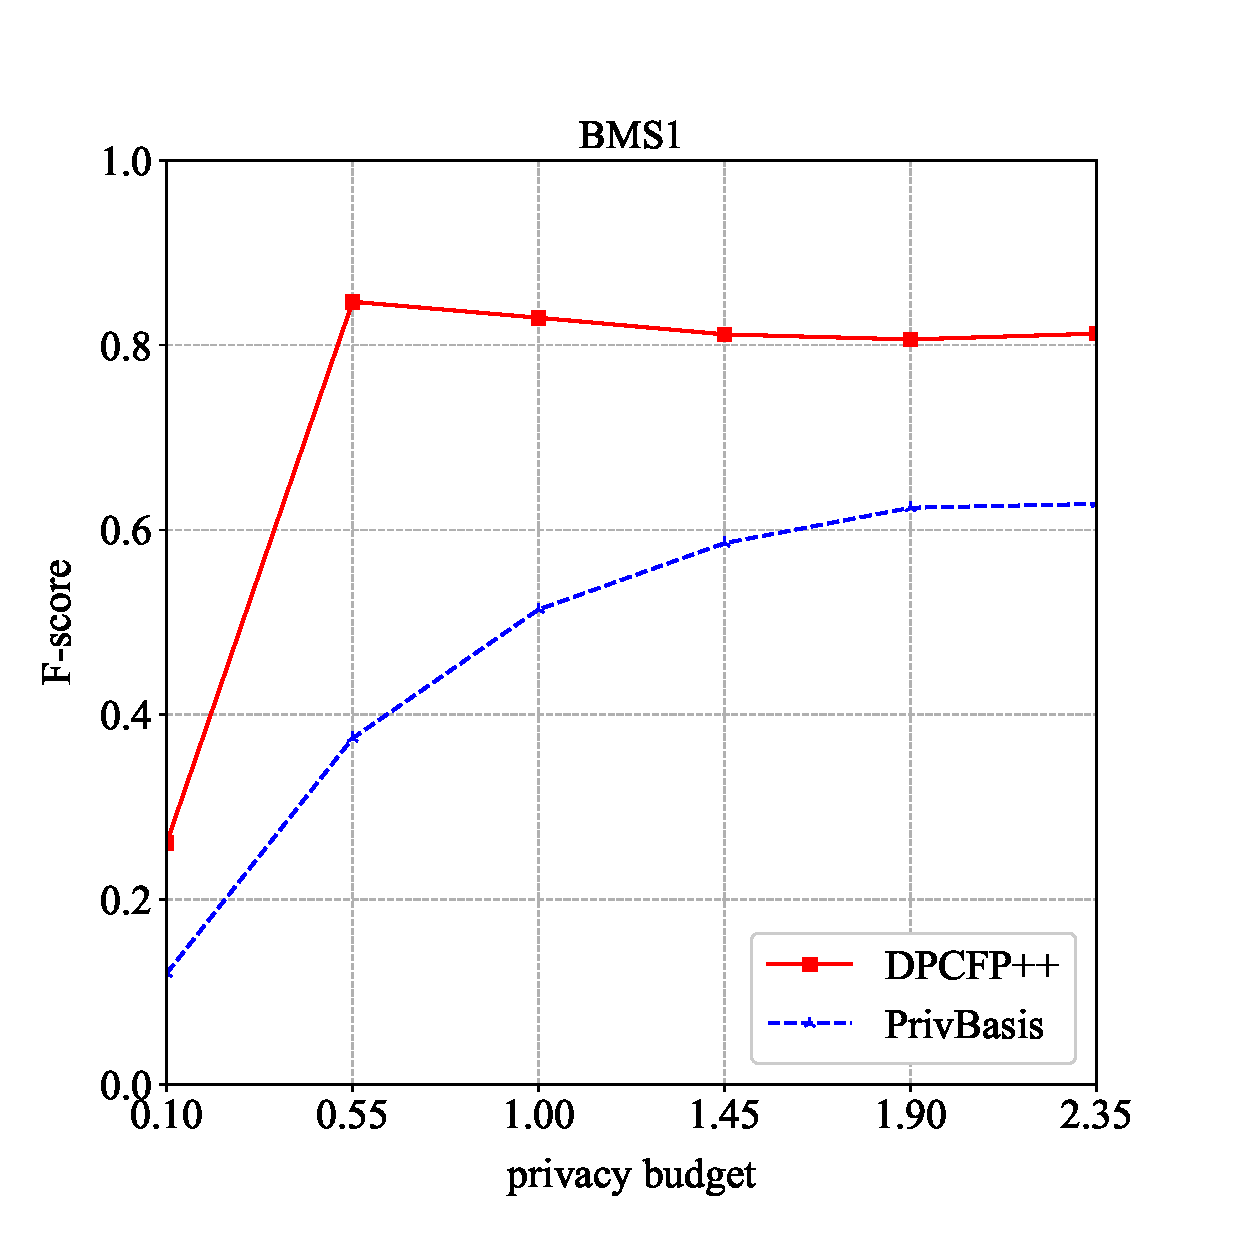
\includegraphics[width=5cm]{F-score_BMS1.eps}
%     \caption{BMS1}
%     \end{minipage}
%     \hfill
%     \begin{minipage}[t]{0.3\textwidth}
%     \centering
%     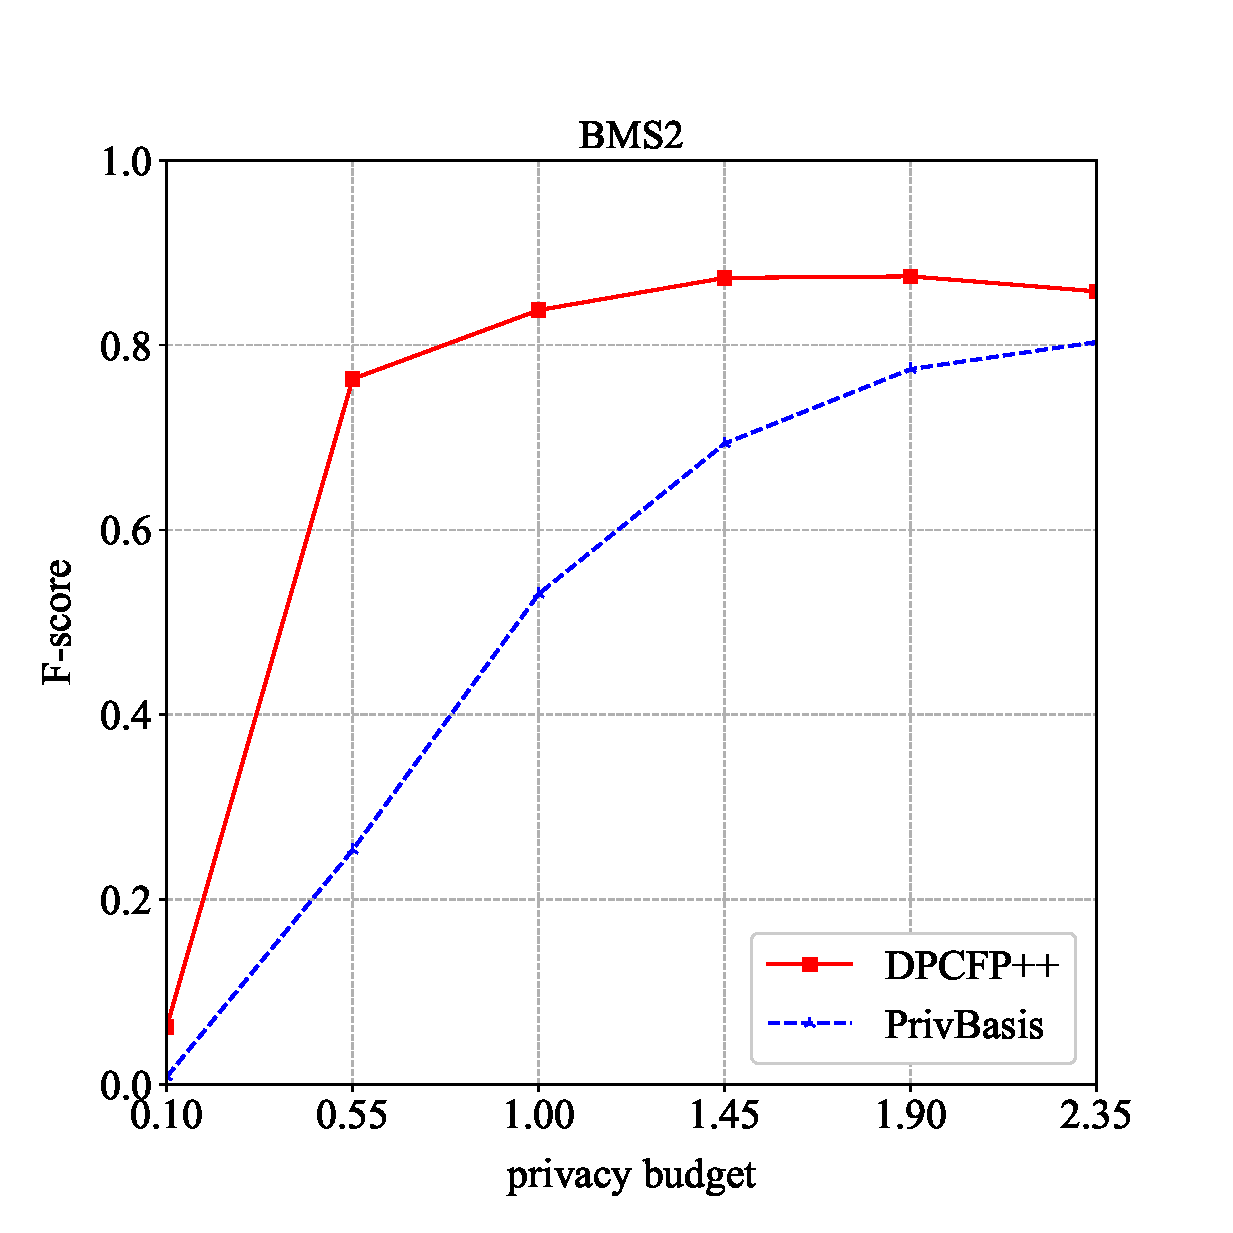
\includegraphics[width=5cm]{F-score_BMS2.eps}
%     \caption{BMS2}
%     \end{minipage}
%     \hfill
%     \begin{minipage}[t]{0.3\textwidth}
%     \centering
%     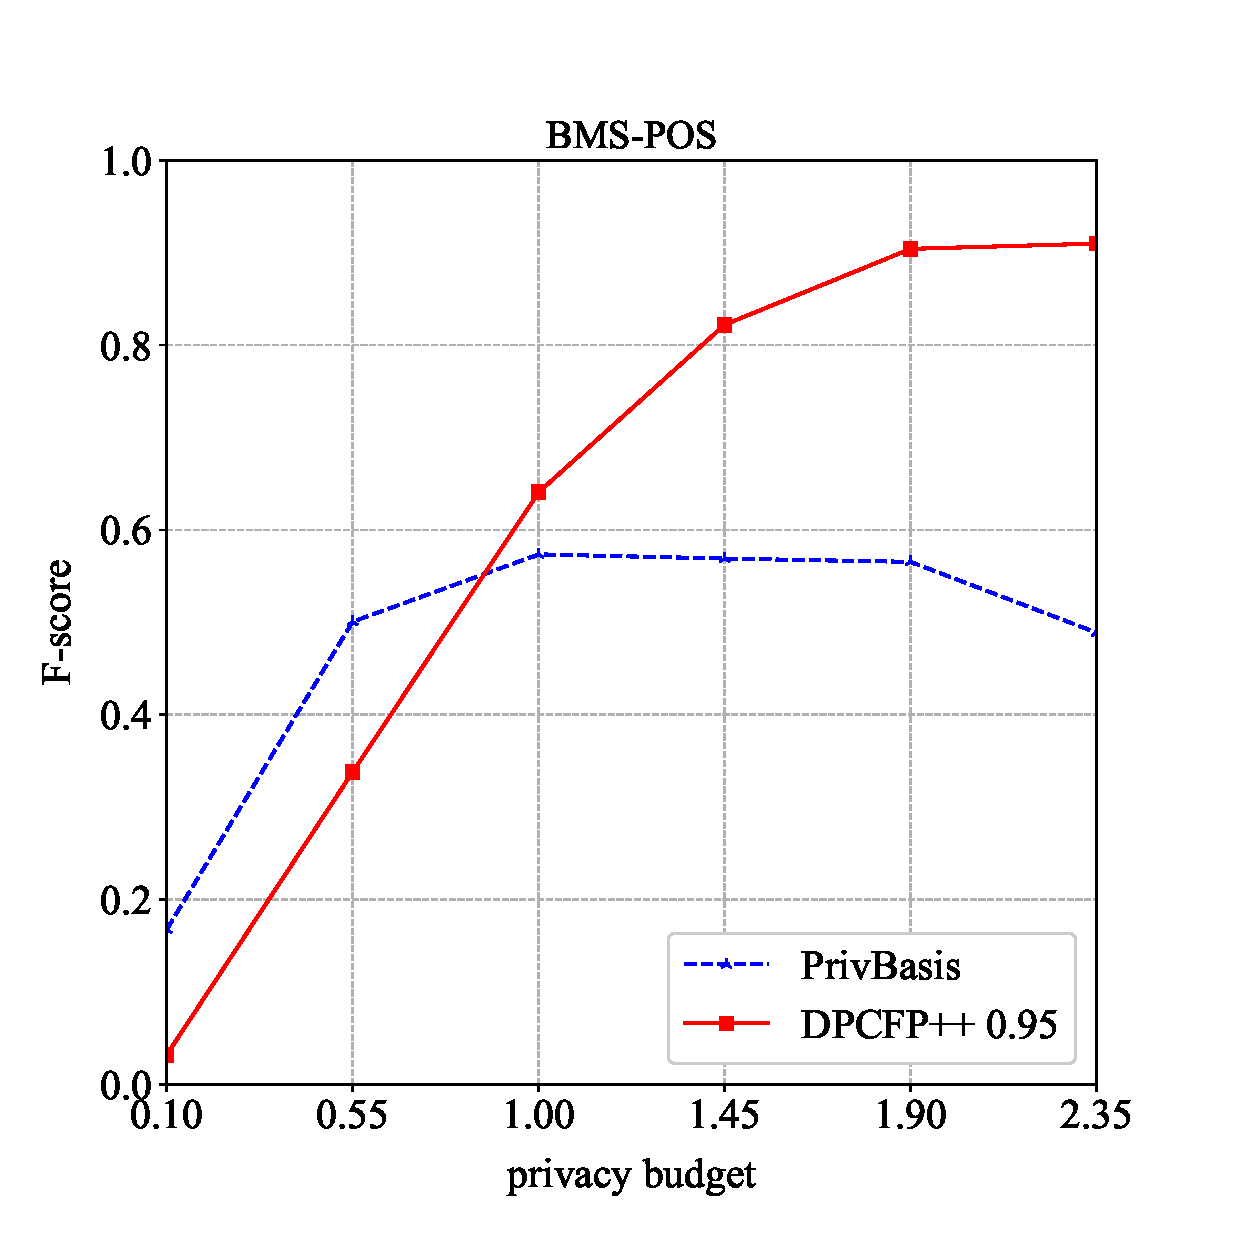
\includegraphics[width=5cm]{F-score_BMS-POS.eps}
%     \caption{BMS-POS}
%     \end{minipage}

%     \begin{minipage}[t]{0.3\textwidth}
%     \centering
%     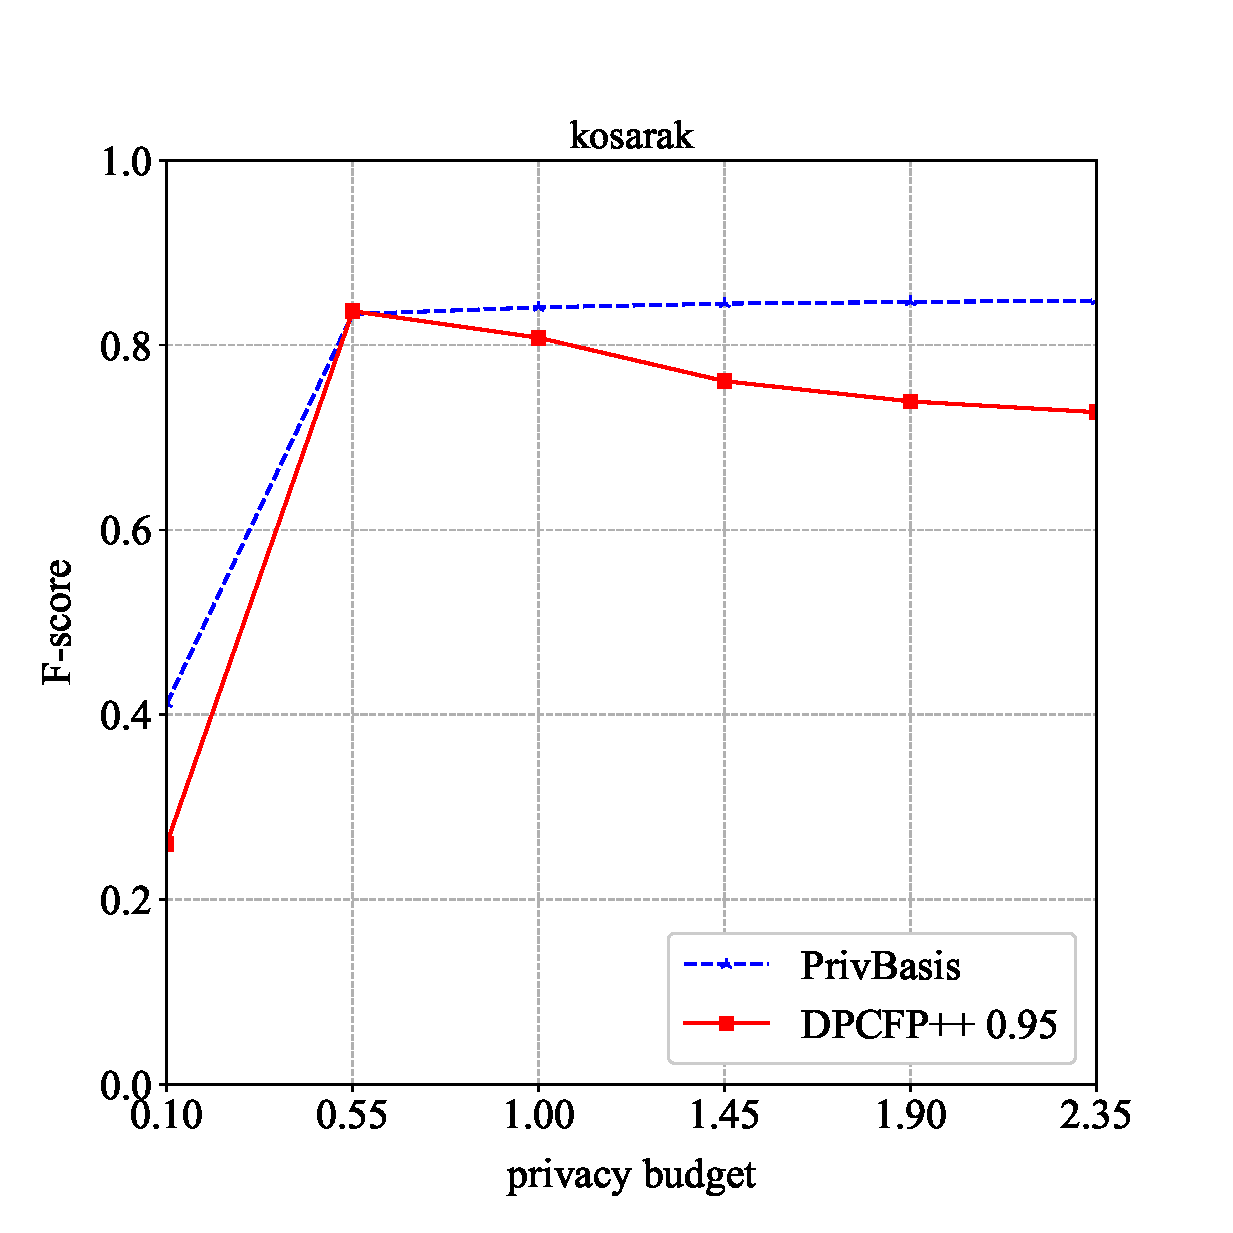
\includegraphics[width=5cm]{F-score_kosarak.eps}
%     % \subcaption{Kosarak}
%     \end{minipage}
%     \hfill
%     \begin{minipage}[t]{0.3\textwidth}
%     \centering
%     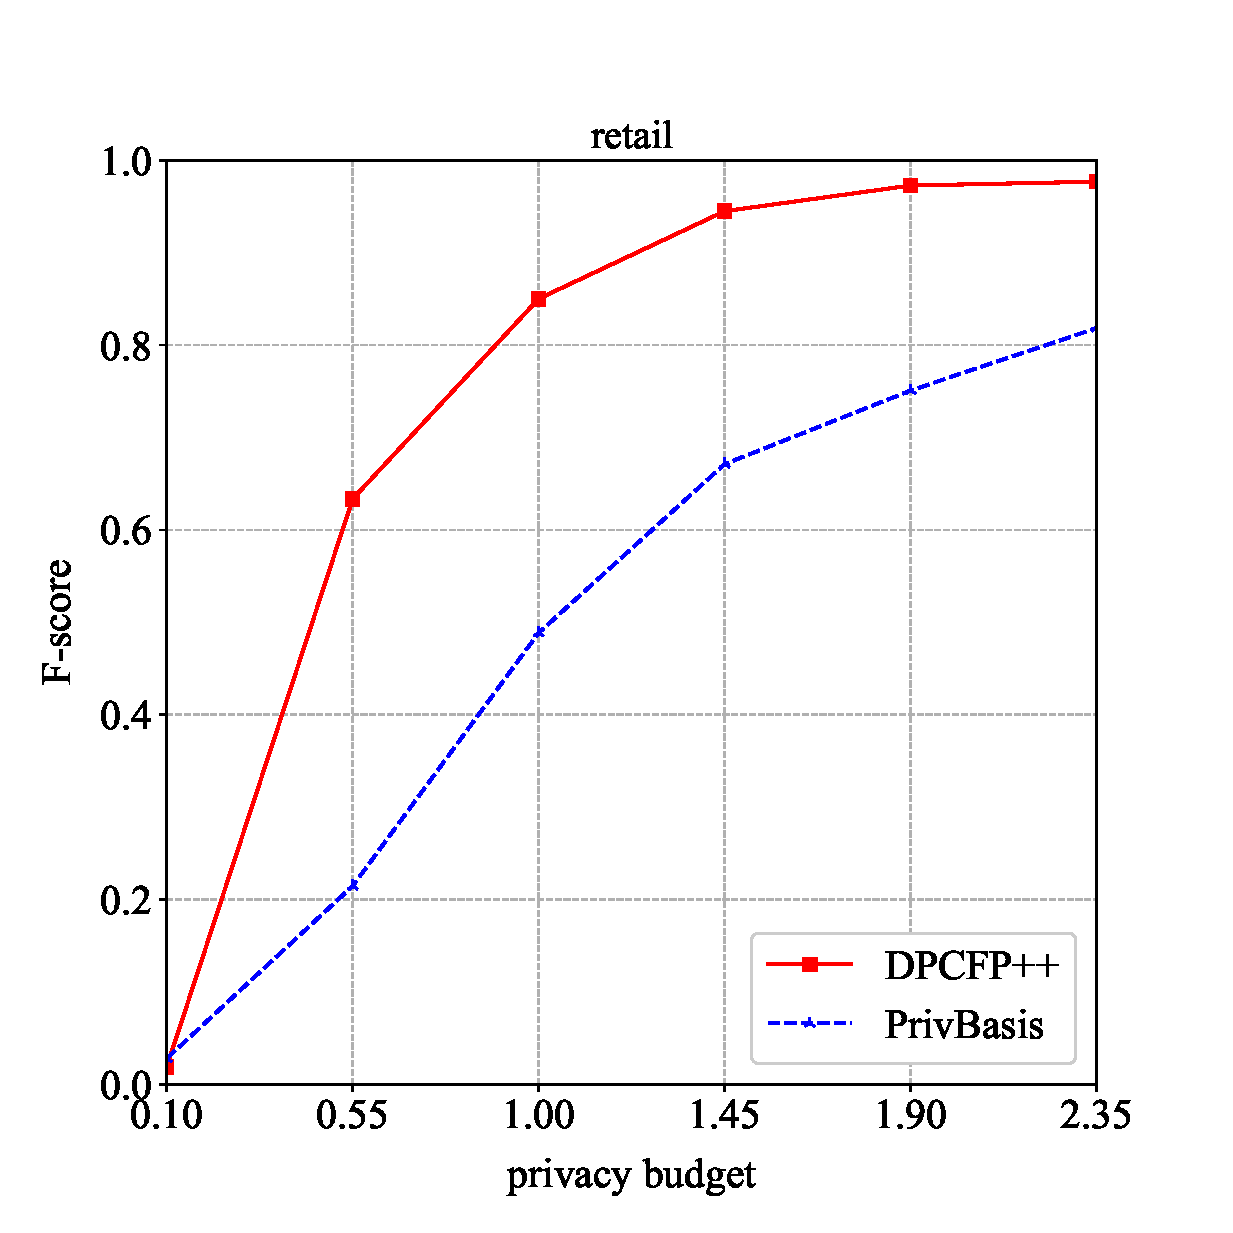
\includegraphics[width=5cm]{F-score_retail.eps}
%     % \subcaption{Retail}
%     \end{minipage}
%     \hfill
%     \begin{minipage}[t]{0.3\textwidth}
%     \centering
%     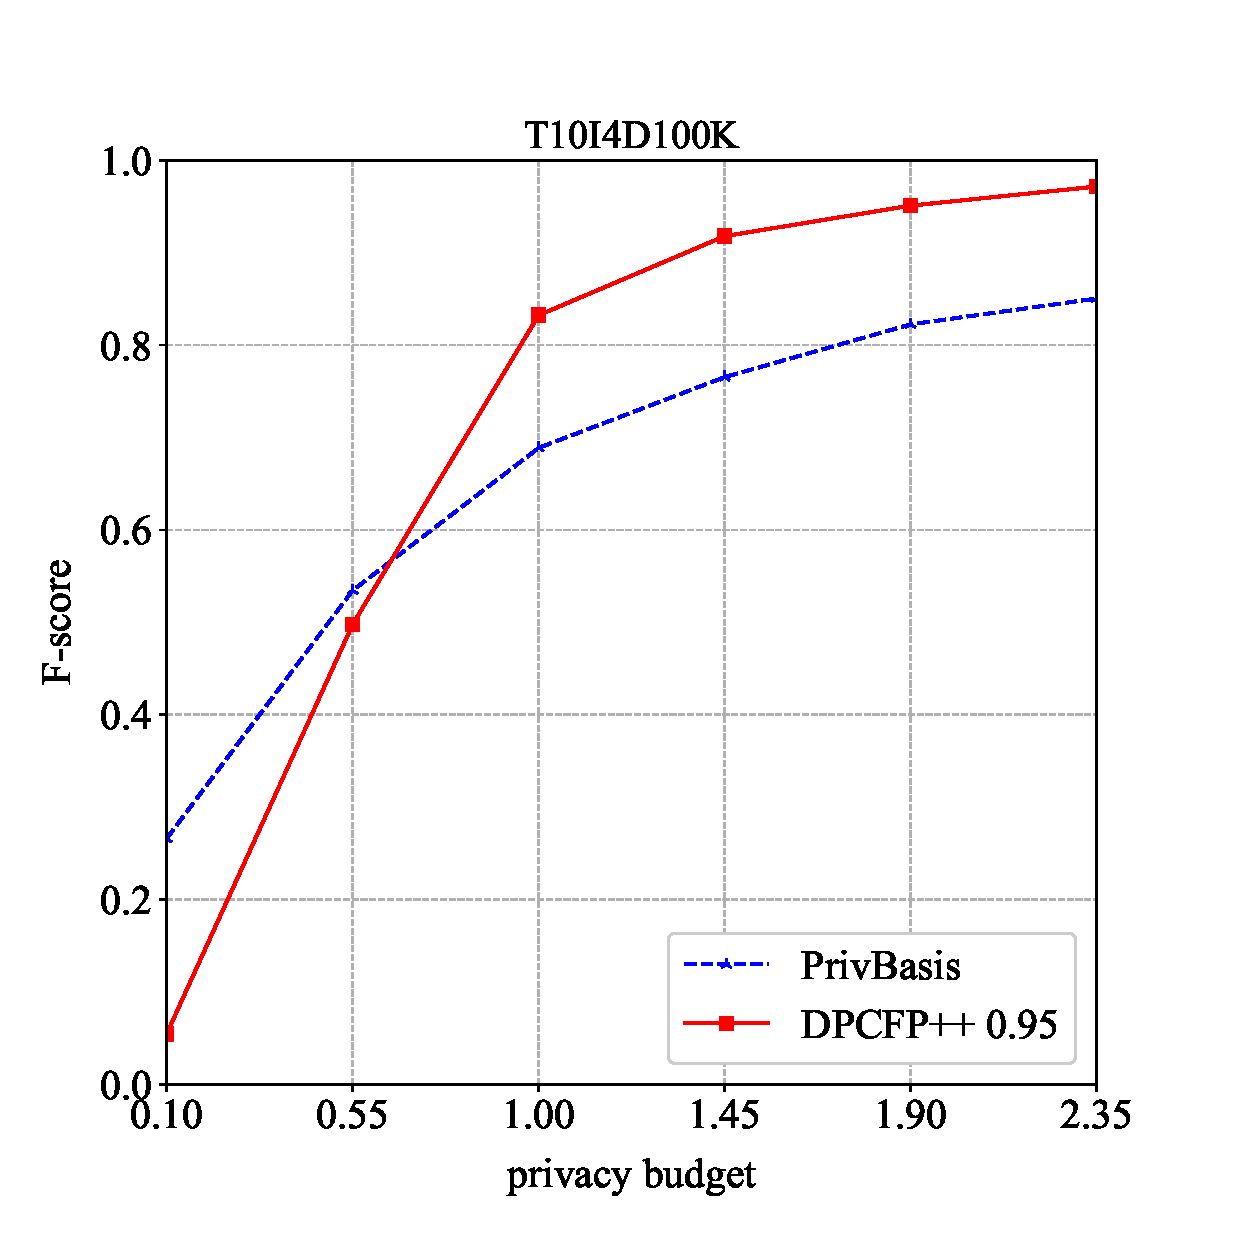
\includegraphics[width=5cm]{F-score_T10I4D100K.eps}
%     % \subcaption{T10I4D100K}
%     \end{minipage}
% \caption{F-score.}
% \label{fig2}
% \end{figure*}

\begin{figure*}[tb]
    \centering
    \subfloat[BMS1]{
        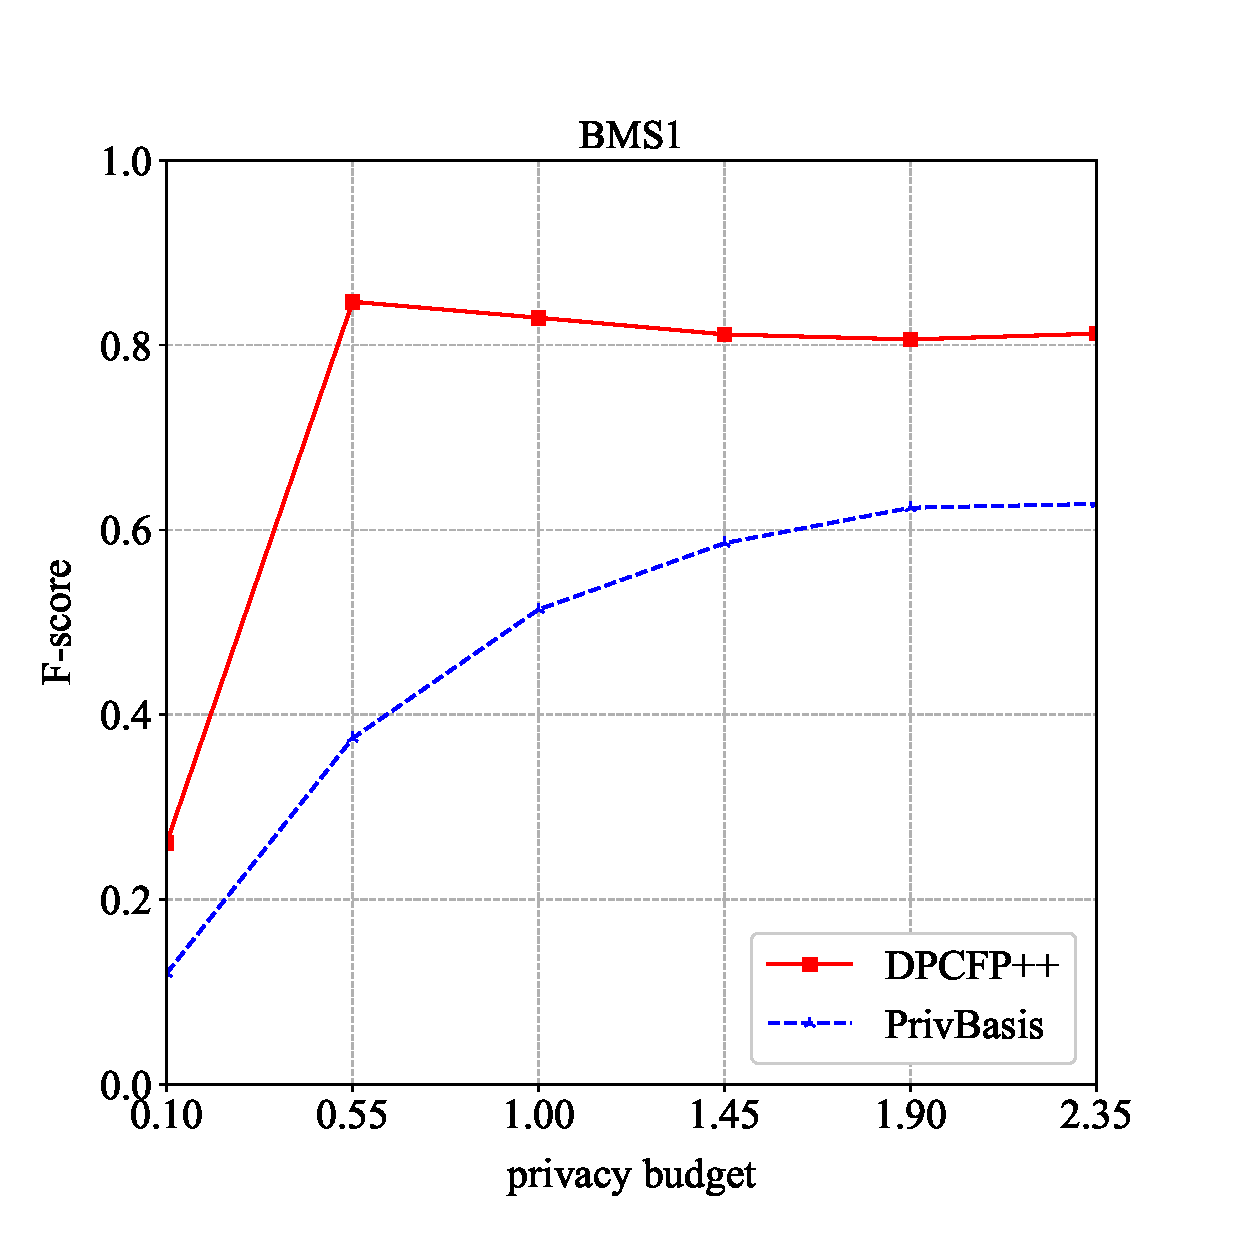
\includegraphics[width=4.5cm]{F-score_BMS1.eps}
    }
    \hfill
    \subfloat[BMS2]{
        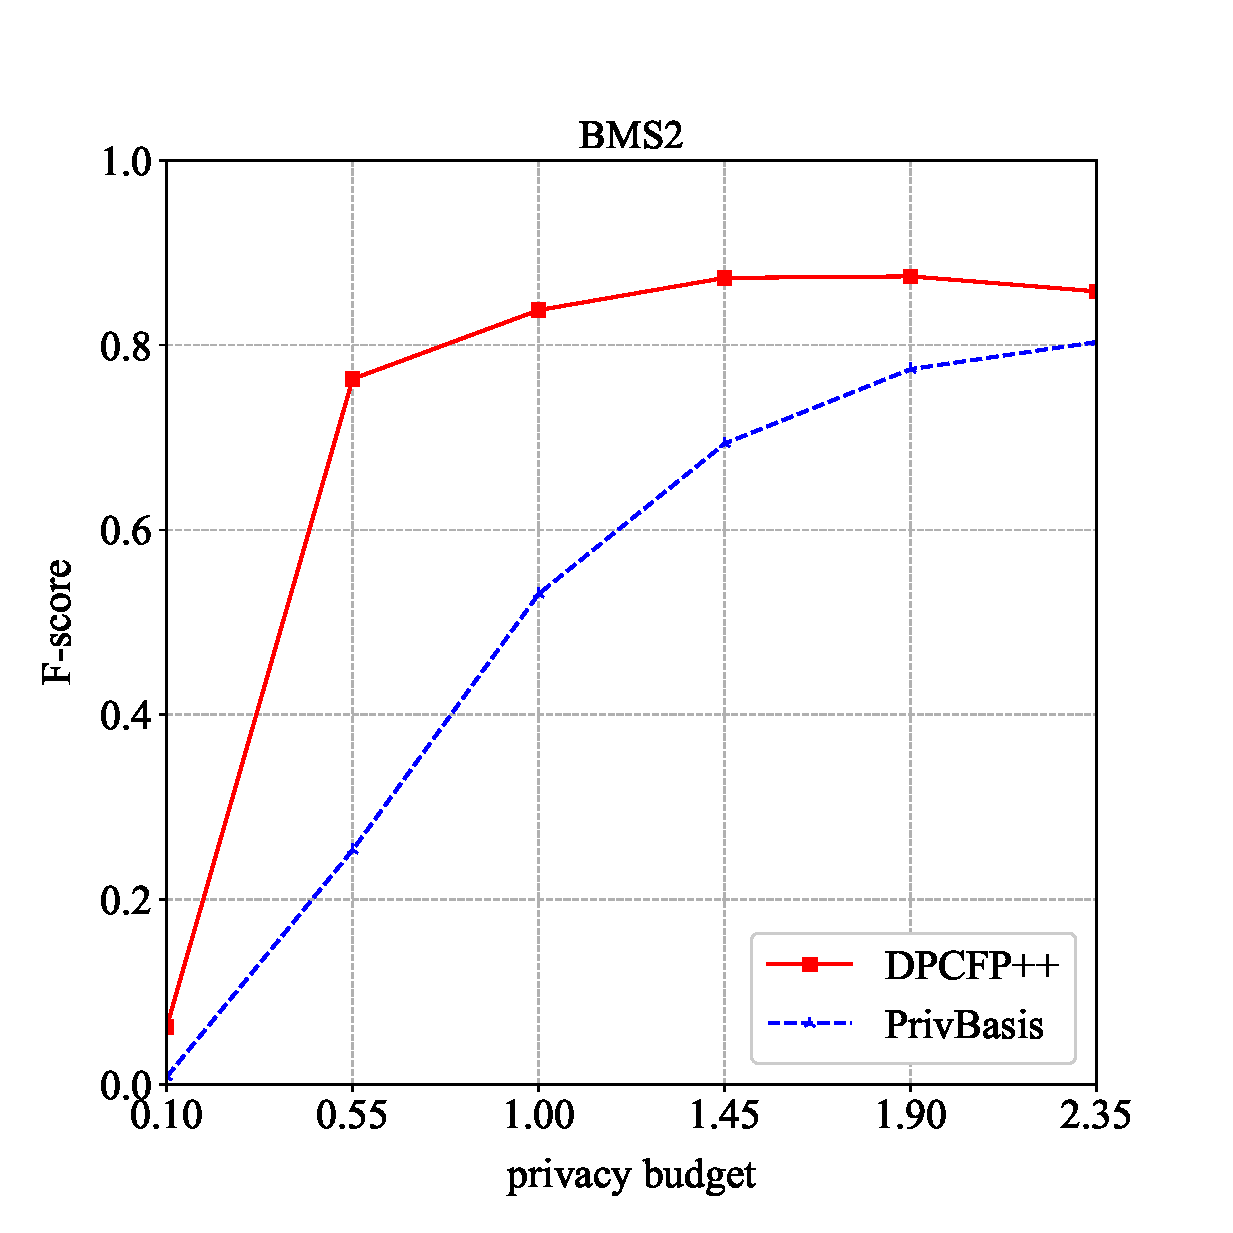
\includegraphics[width=4.5cm]{F-score_BMS2.eps}
    }
    \hfill
    \subfloat[BMS-POS]{
        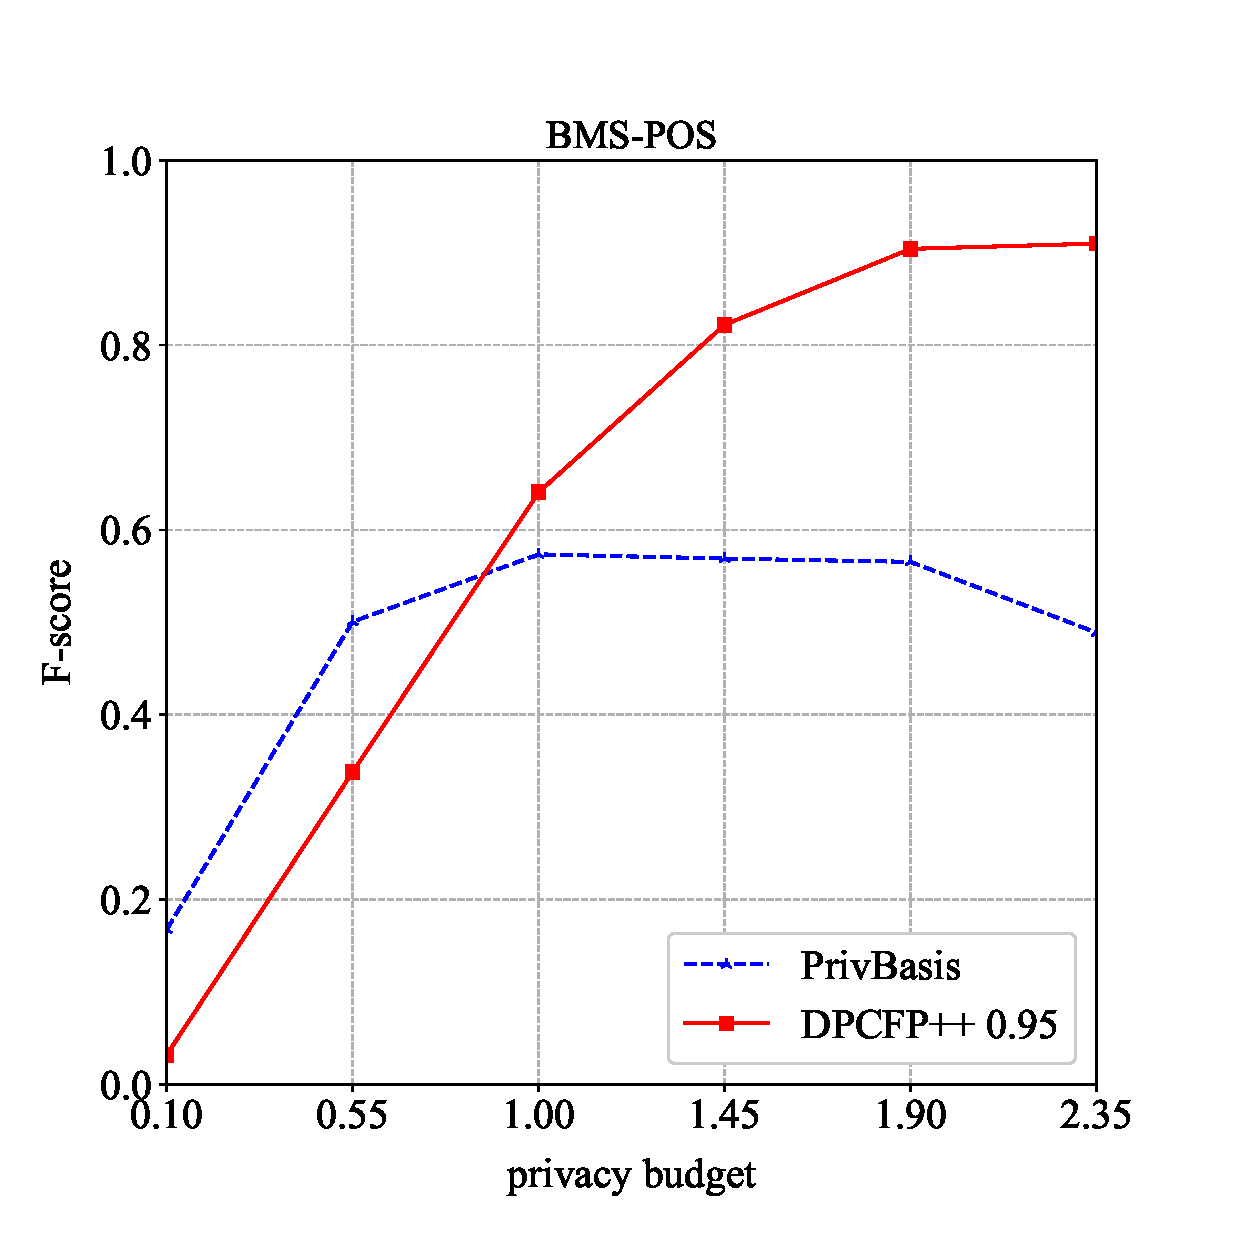
\includegraphics[width=4.5cm]{F-score_BMS-POS.eps}
    }
    \\
    \subfloat[Kosarak]{
        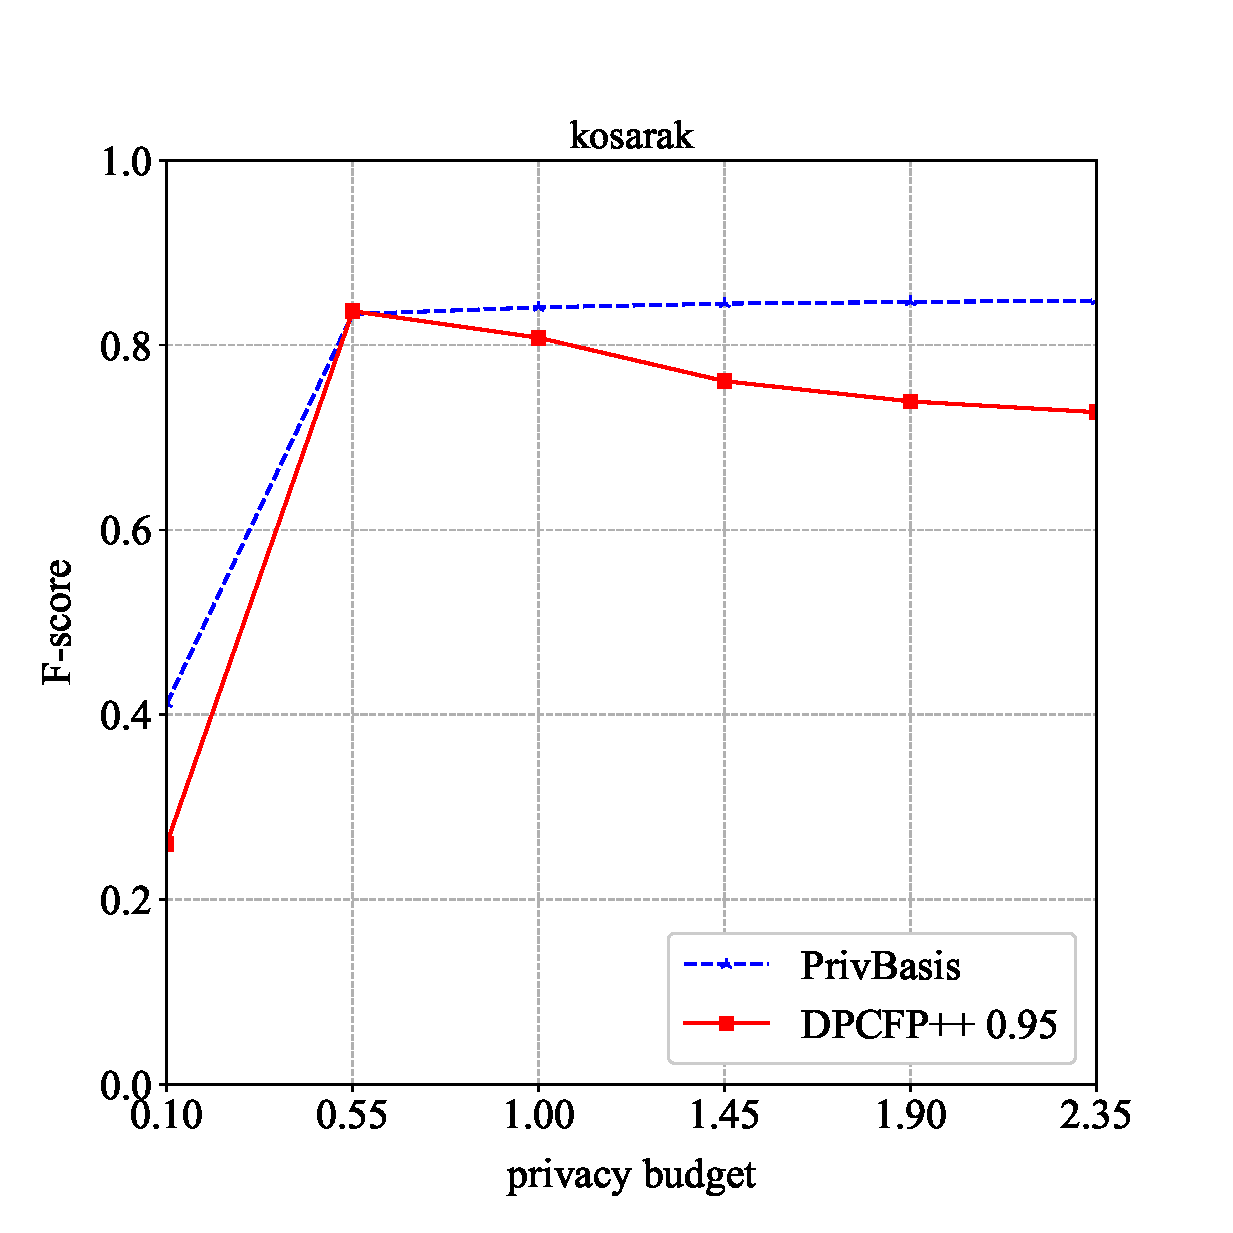
\includegraphics[width=4.5cm]{F-score_kosarak.eps}
    }
    \hfill
    \subfloat[Retail]{
        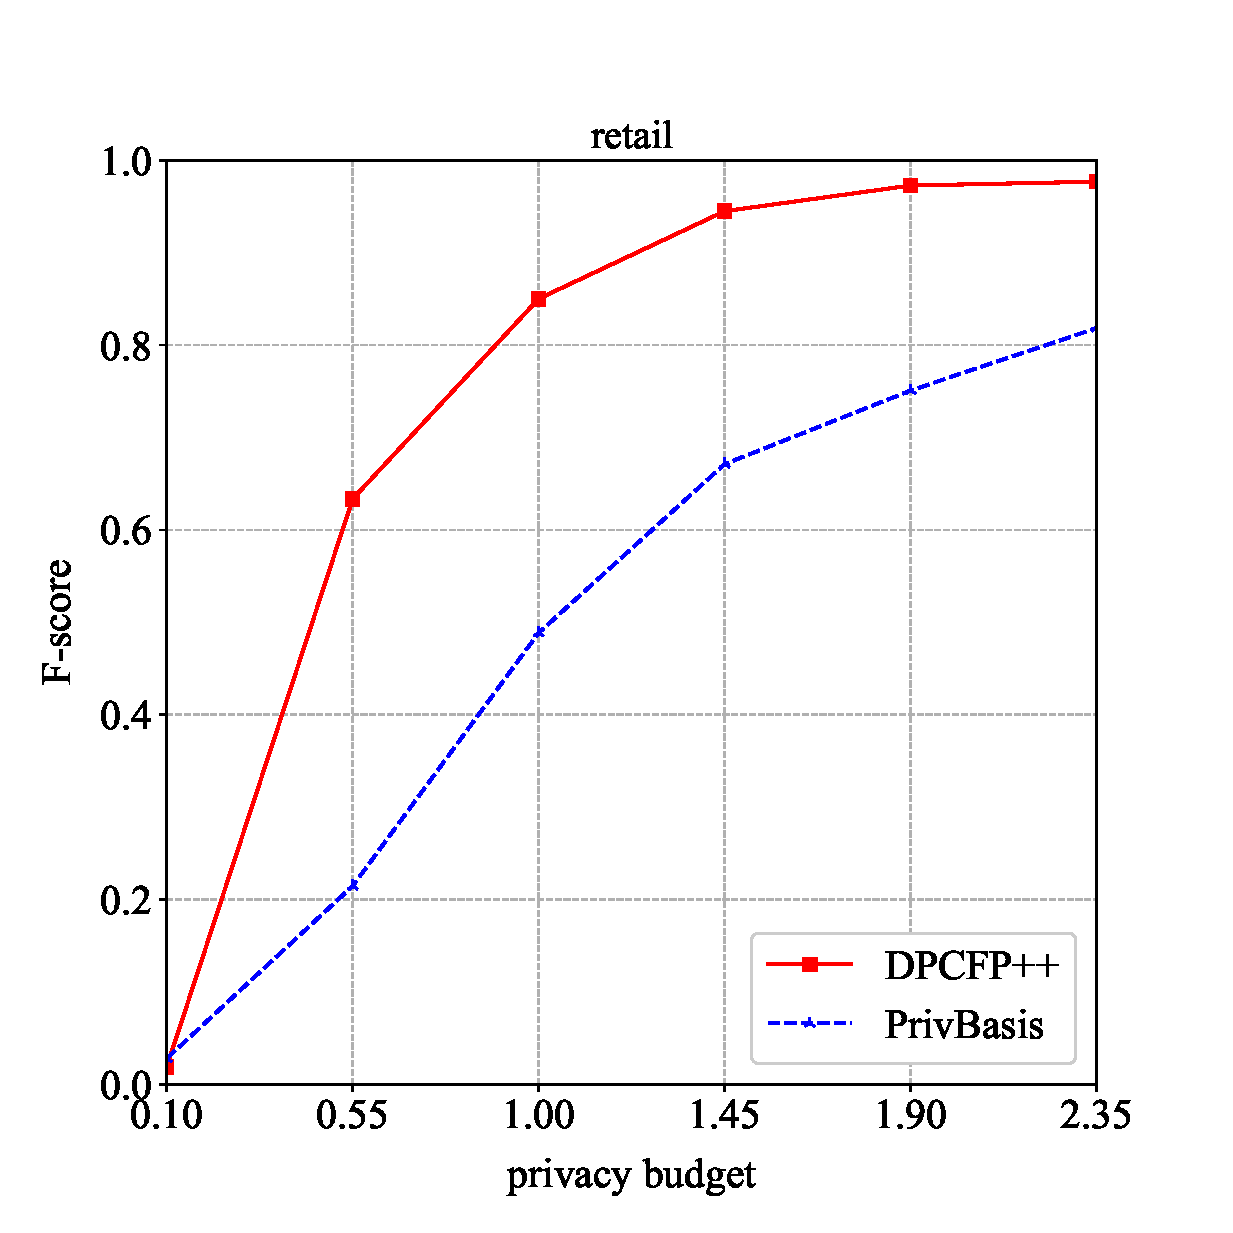
\includegraphics[width=4.5cm]{F-score_retail.eps}
    }
    \hfill
    \subfloat[T10I4D100K]{
        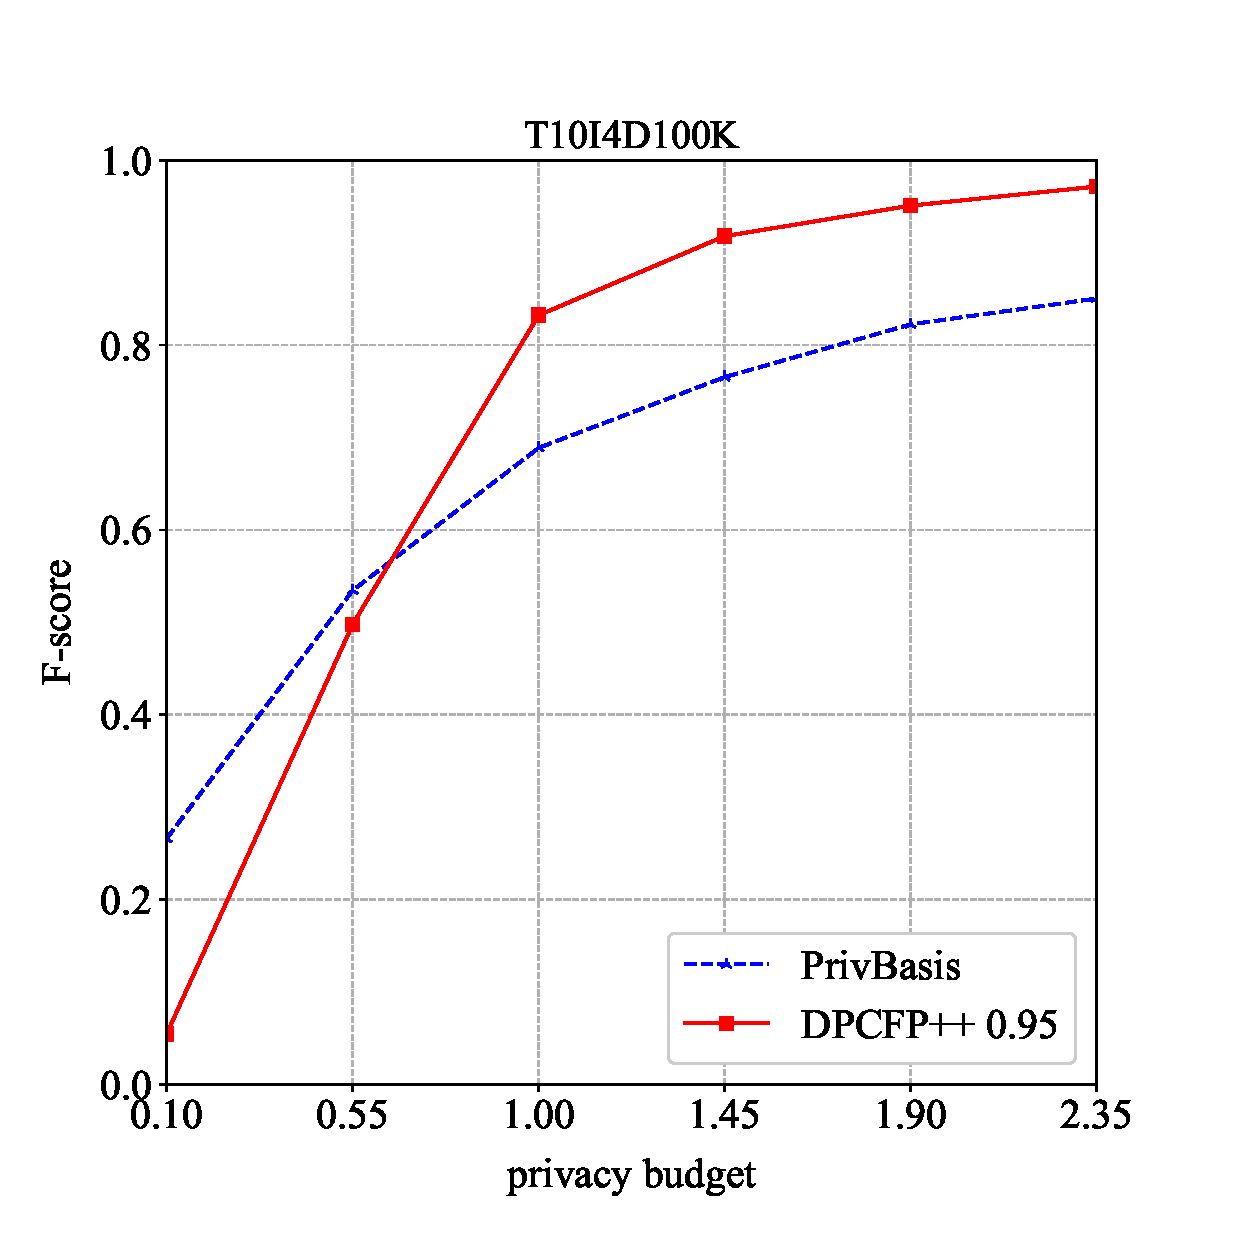
\includegraphics[width=4.5cm]{F-score_T10I4D100K.eps}
    }
\caption{F-score}
\label{fscore}
\end{figure*}

\begin{figure*}[tb]
    \centering
    \subfloat[BMS1]{
        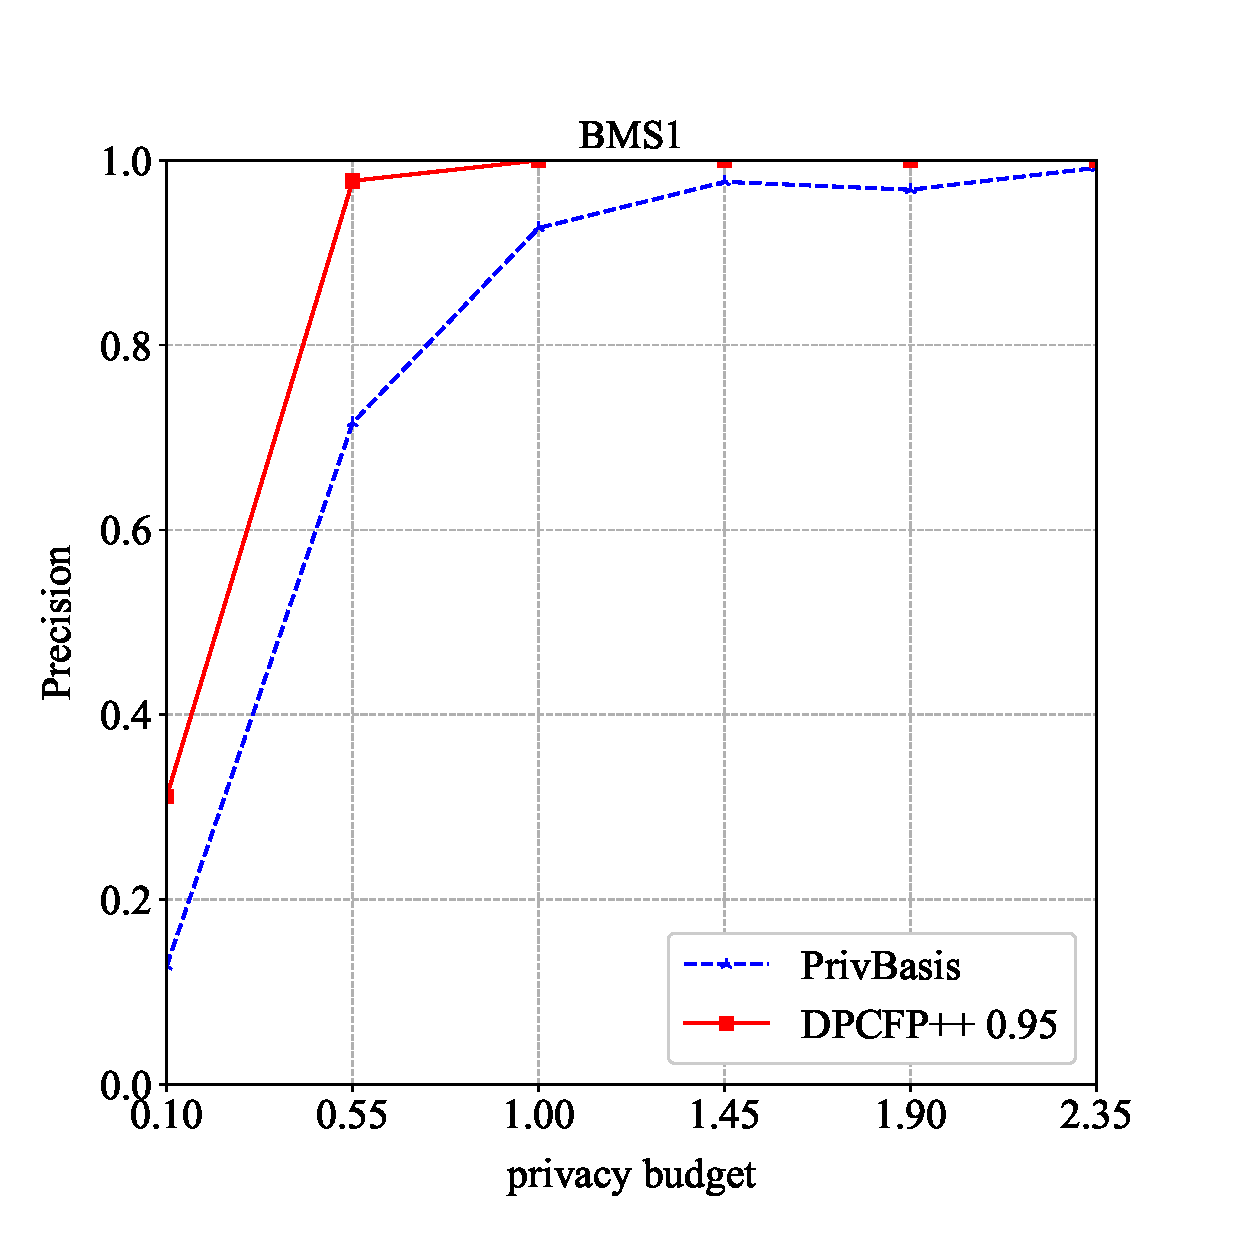
\includegraphics[width=4.5cm]{Precision_BMS1.eps}
    }
    \hfill
    \centering
    \subfloat[BMS2]{
        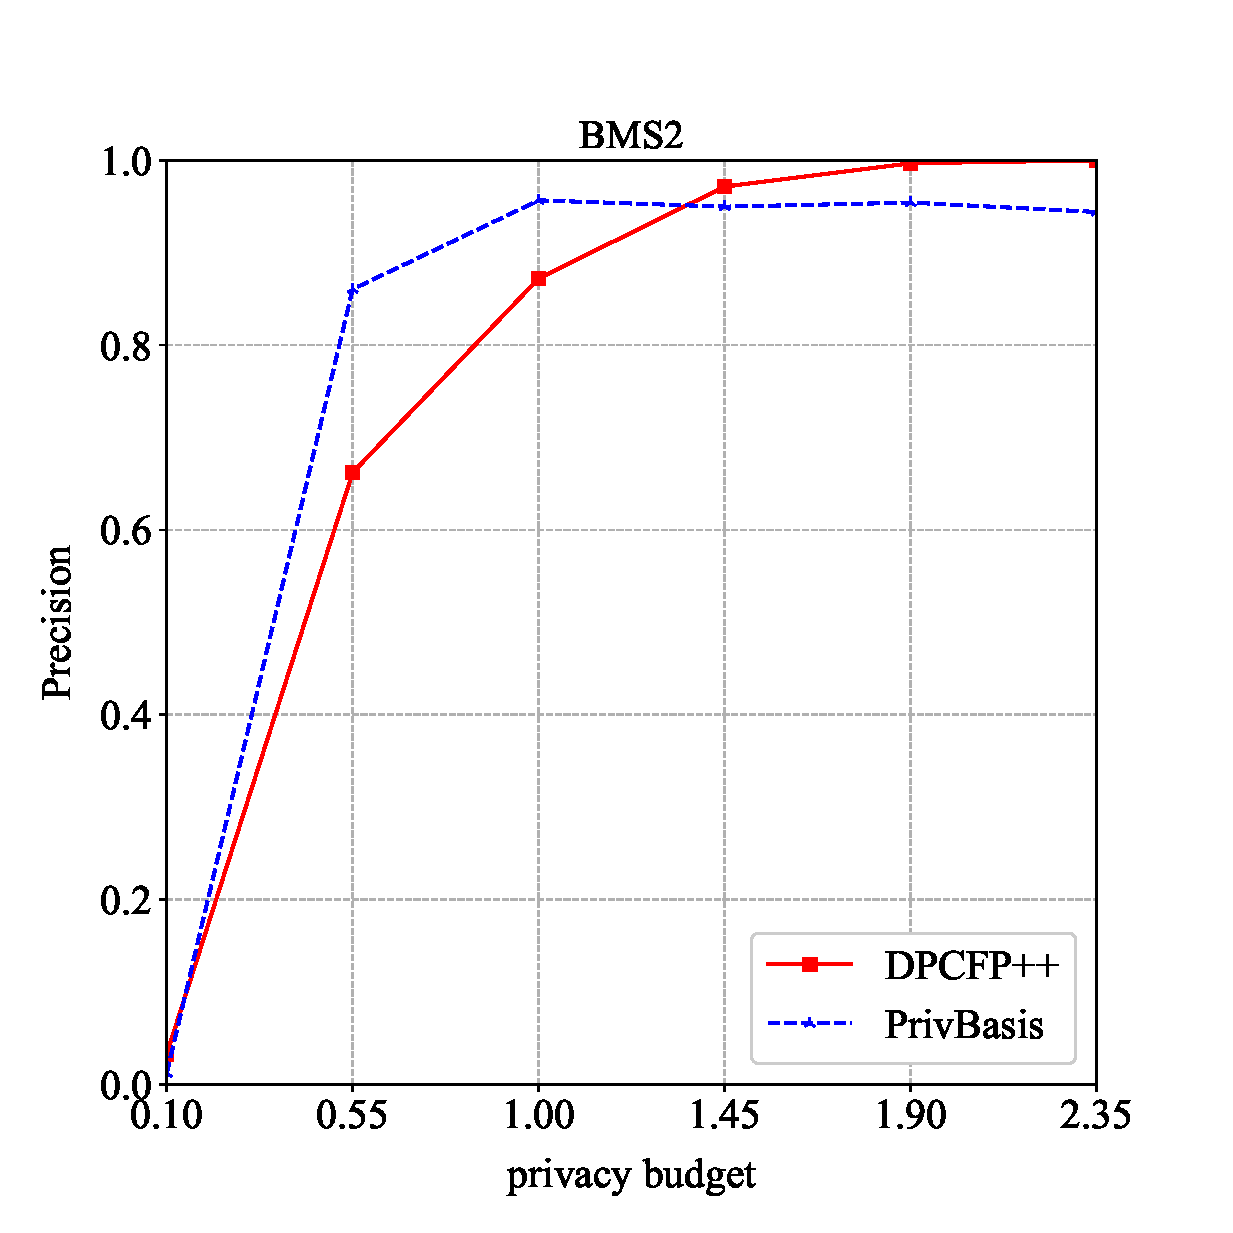
\includegraphics[width=4.5cm]{Precision_BMS2.eps}
    }
    \hfill
    \centering
    \subfloat[BMS-POS]{
        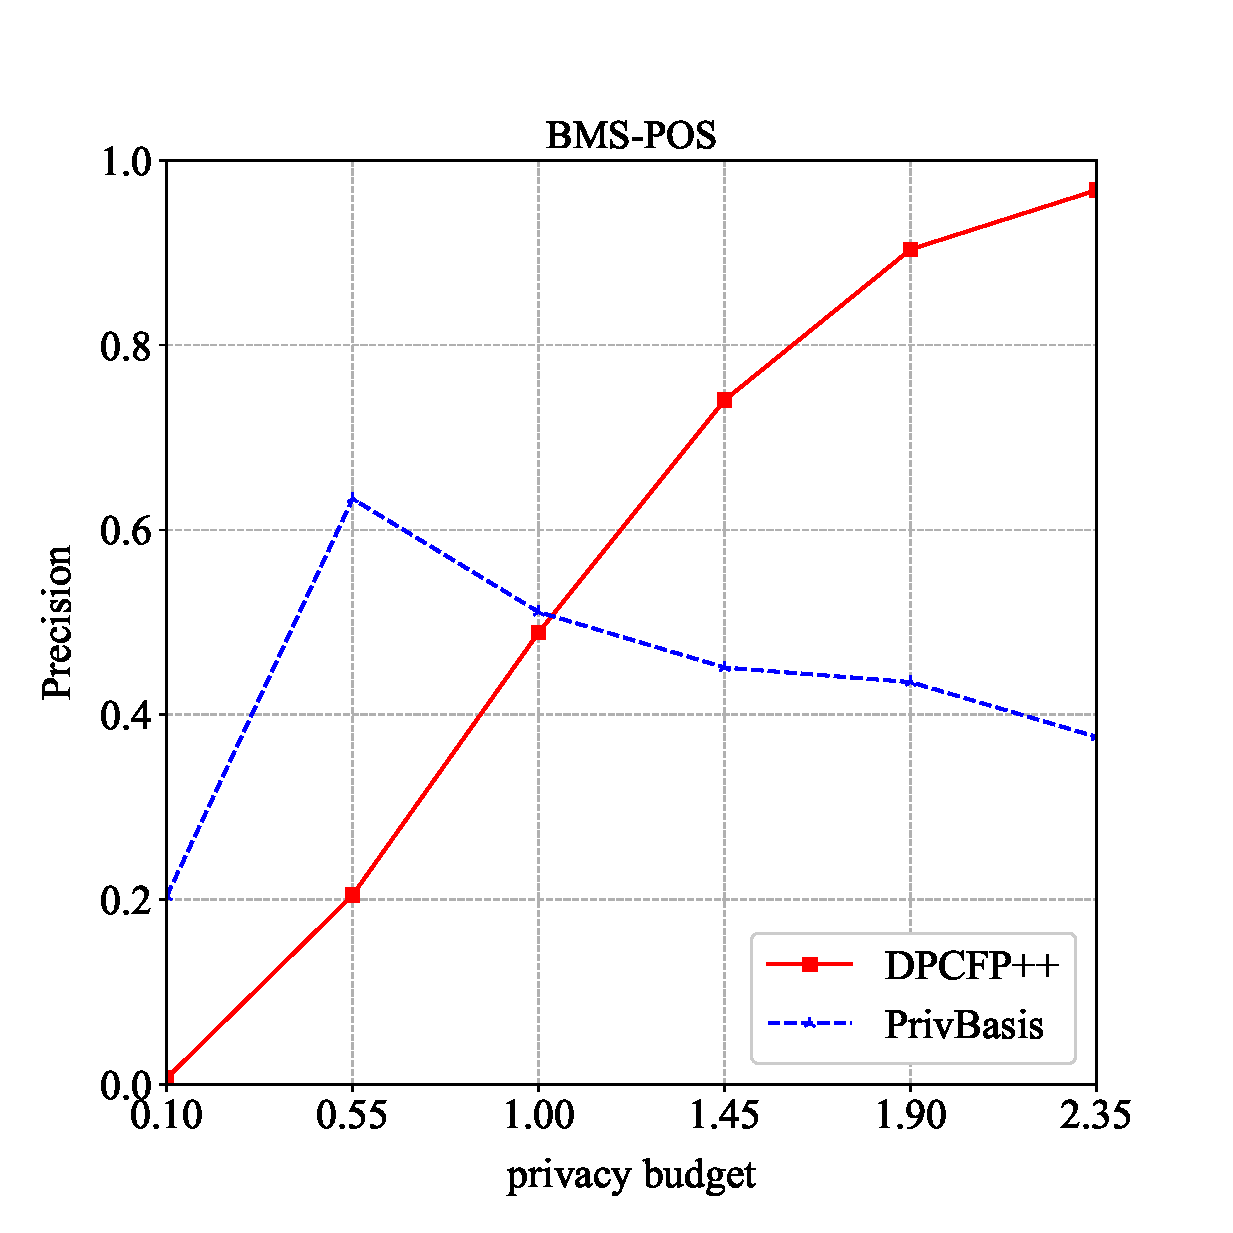
\includegraphics[width=4.5cm]{Precision_BMS-POS.eps}
    }
    \\
    \centering
    \subfloat[Kosarak]{
        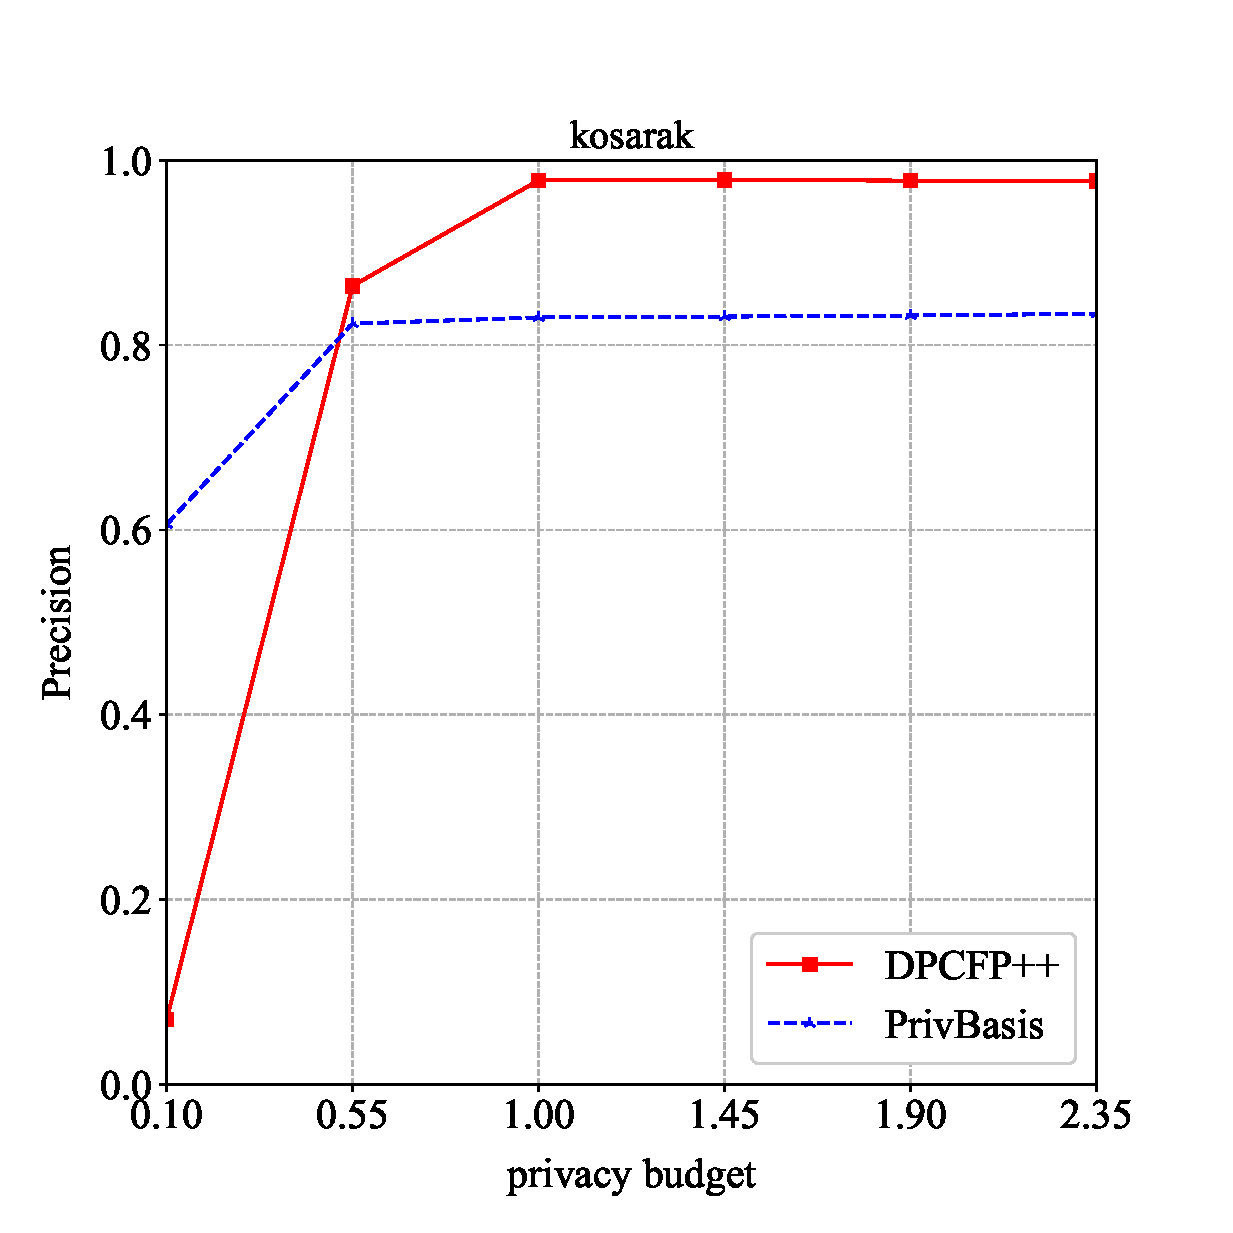
\includegraphics[width=4.5cm]{Precision_kosarak.eps}
    }
    \hfill
    \centering
    \subfloat[Retail]{
        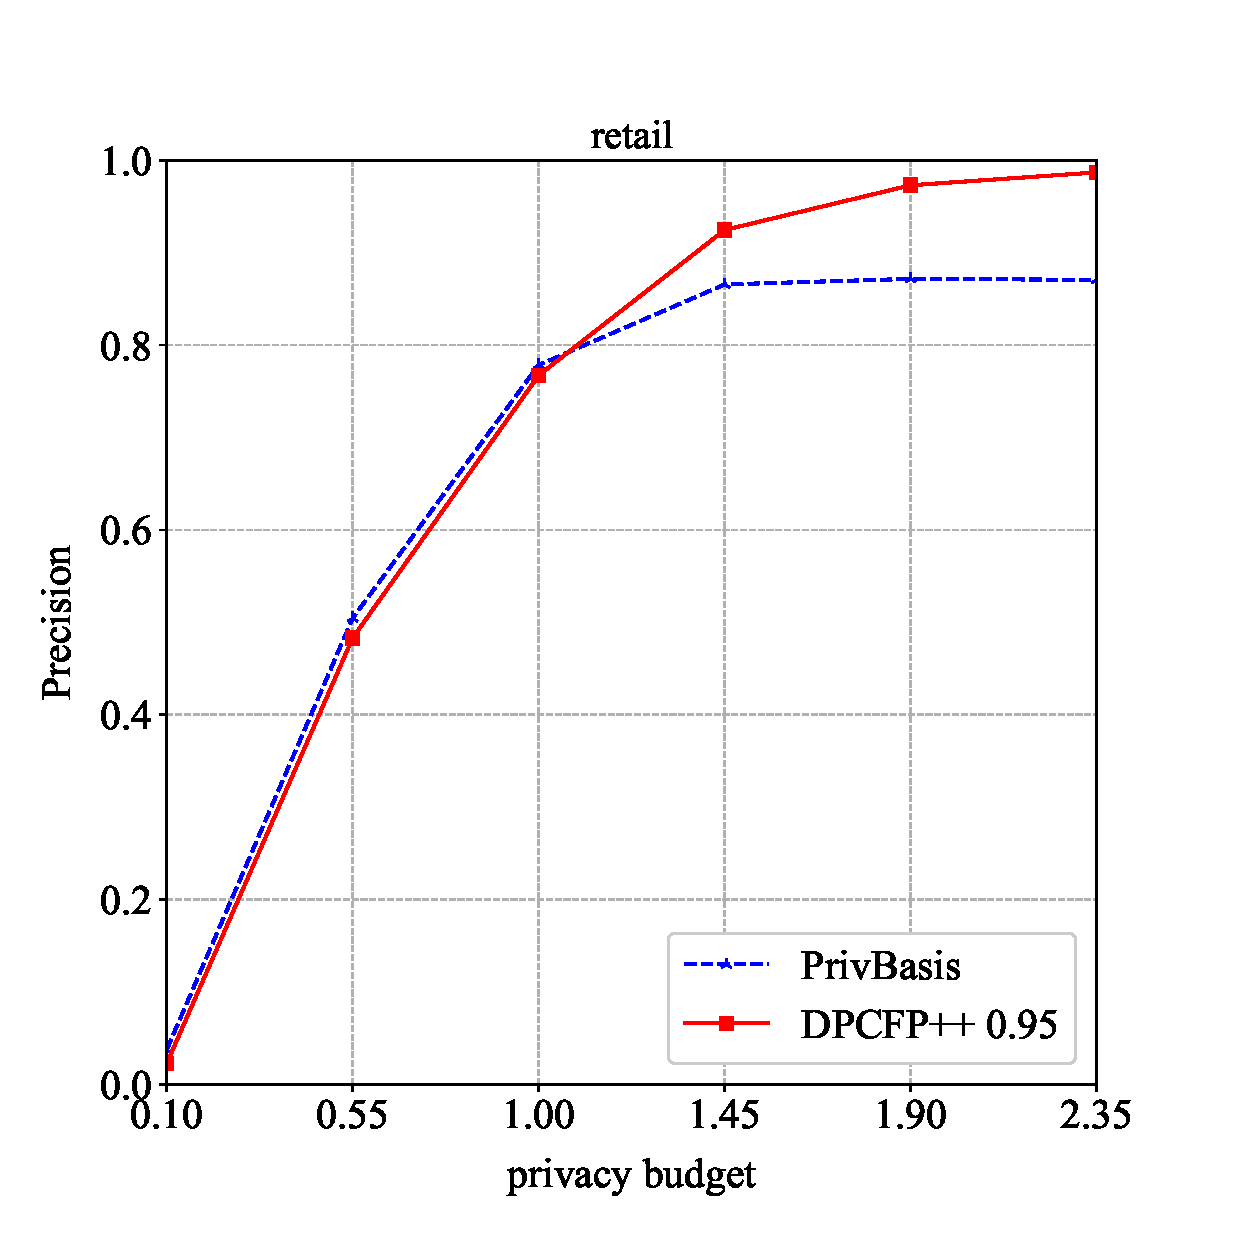
\includegraphics[width=4.5cm]{Precision_retail.eps}
    }
    \hfill
    \centering
    \subfloat[T10I4D100K]{
        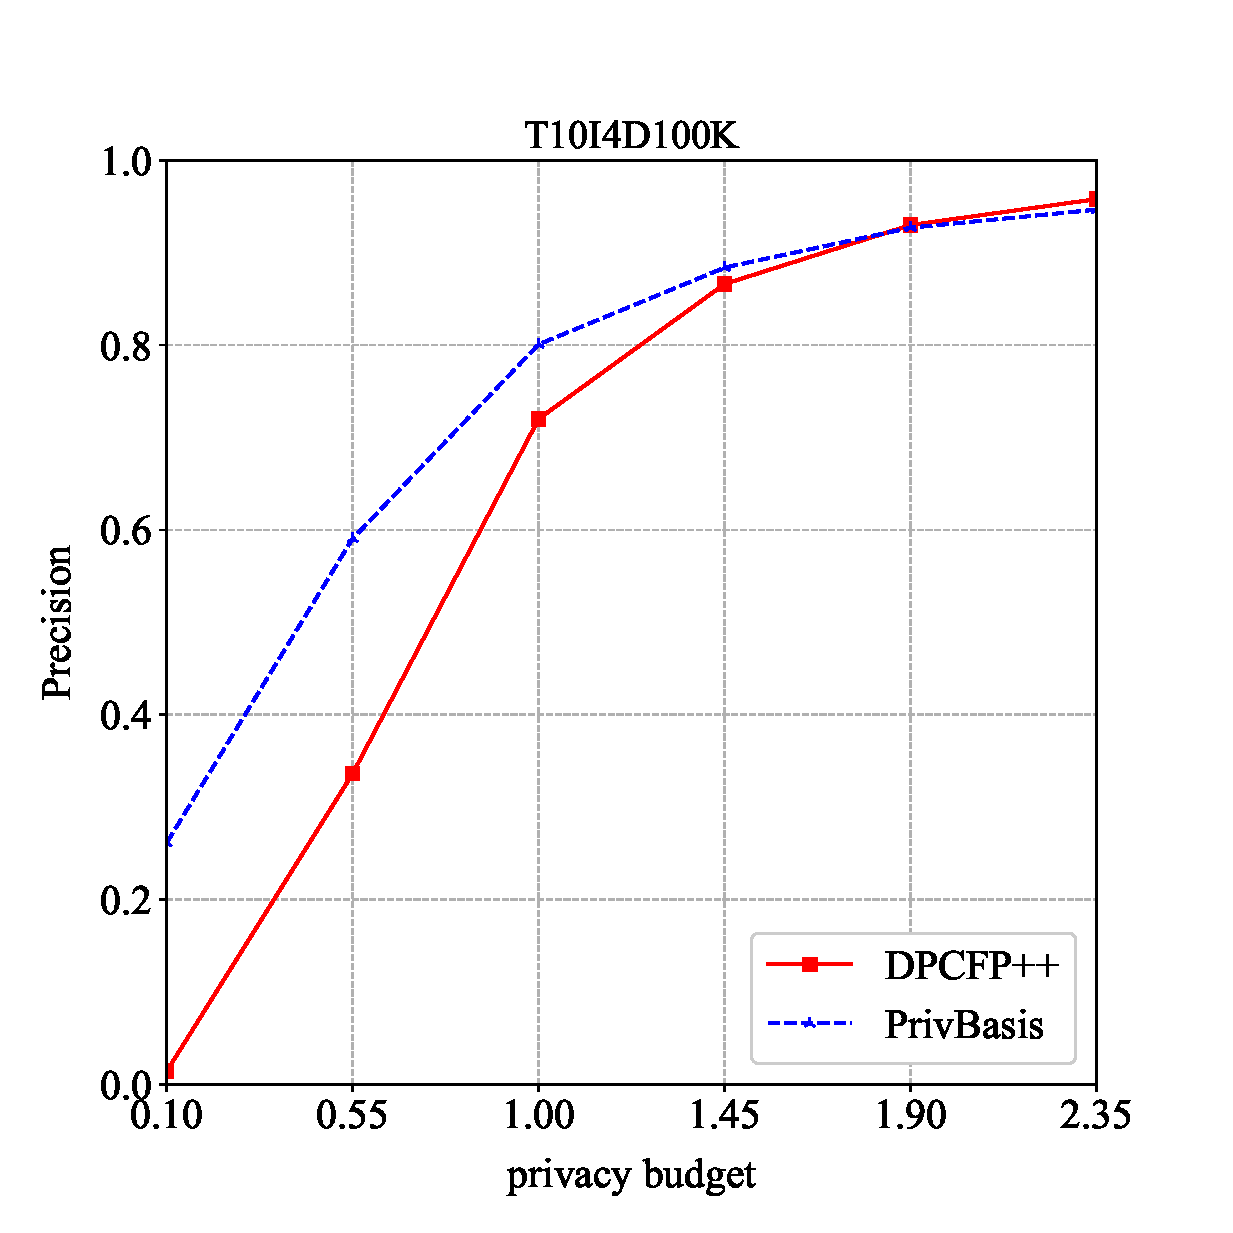
\includegraphics[width=4.5cm]{Precision_T10I4D100K.eps}
    }
\caption{Precision}
\label{Precision}
\end{figure*}

\begin{figure*}[tb]
    \centering
    \subfloat[BMS1]{
        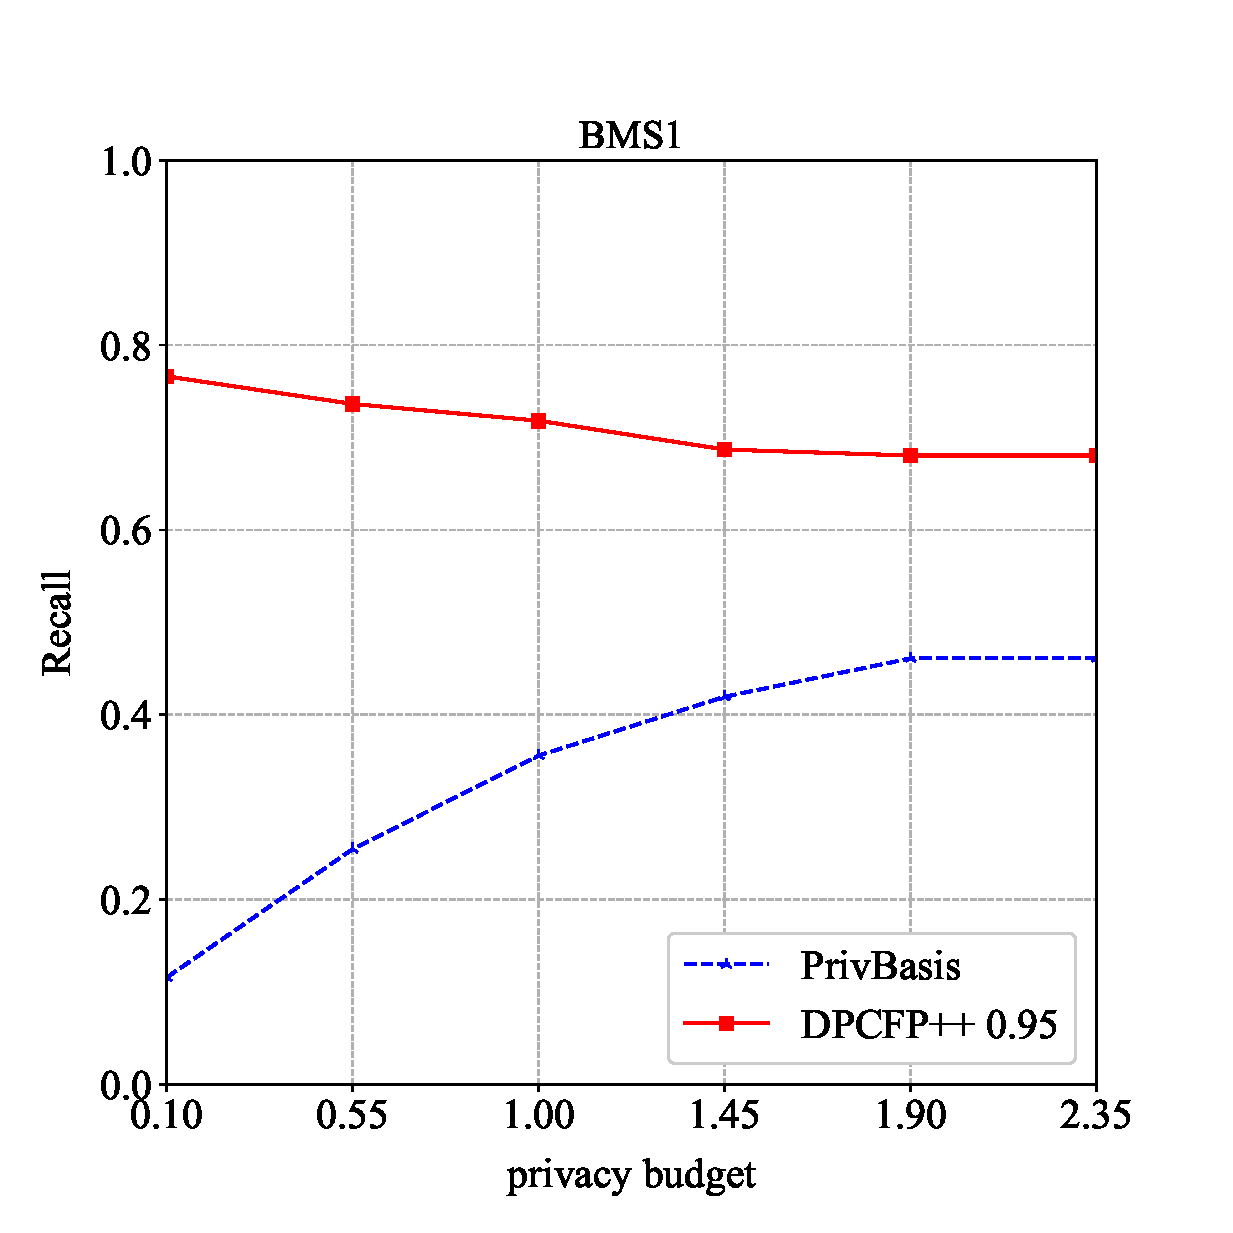
\includegraphics[width=4.5cm]{Recall_BMS1.eps}
    }
    \hfill
    \subfloat[BMS2]{
        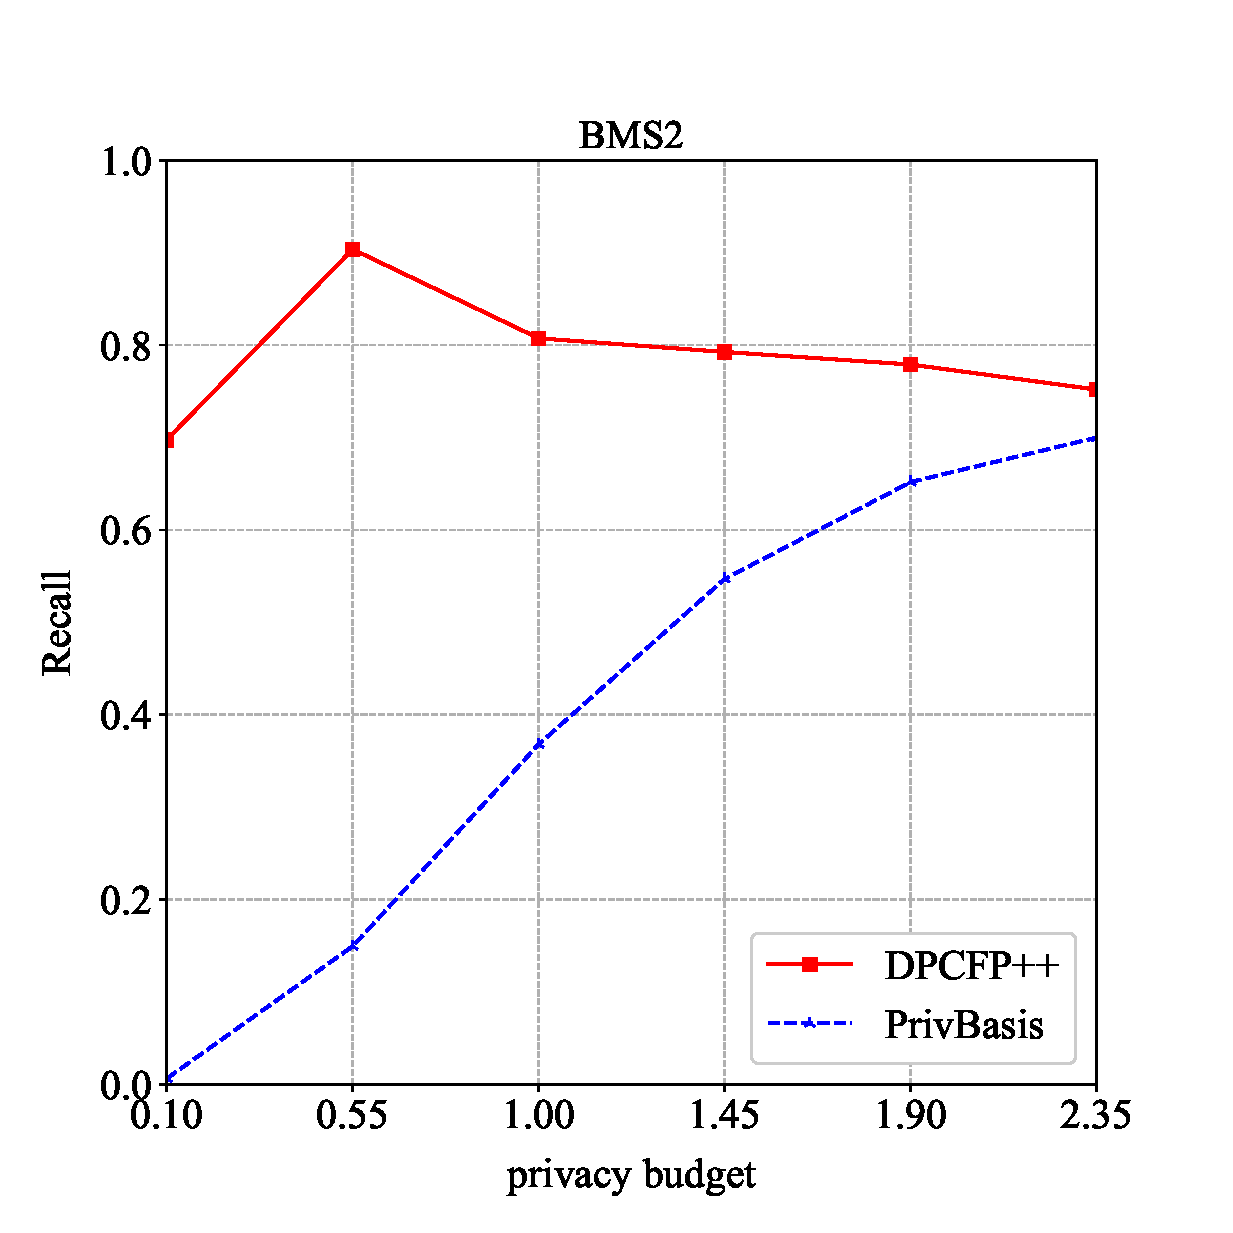
\includegraphics[width=4.5cm]{Recall_BMS2.eps}
    }
    \hfill
    \subfloat[BMS-POS]{
        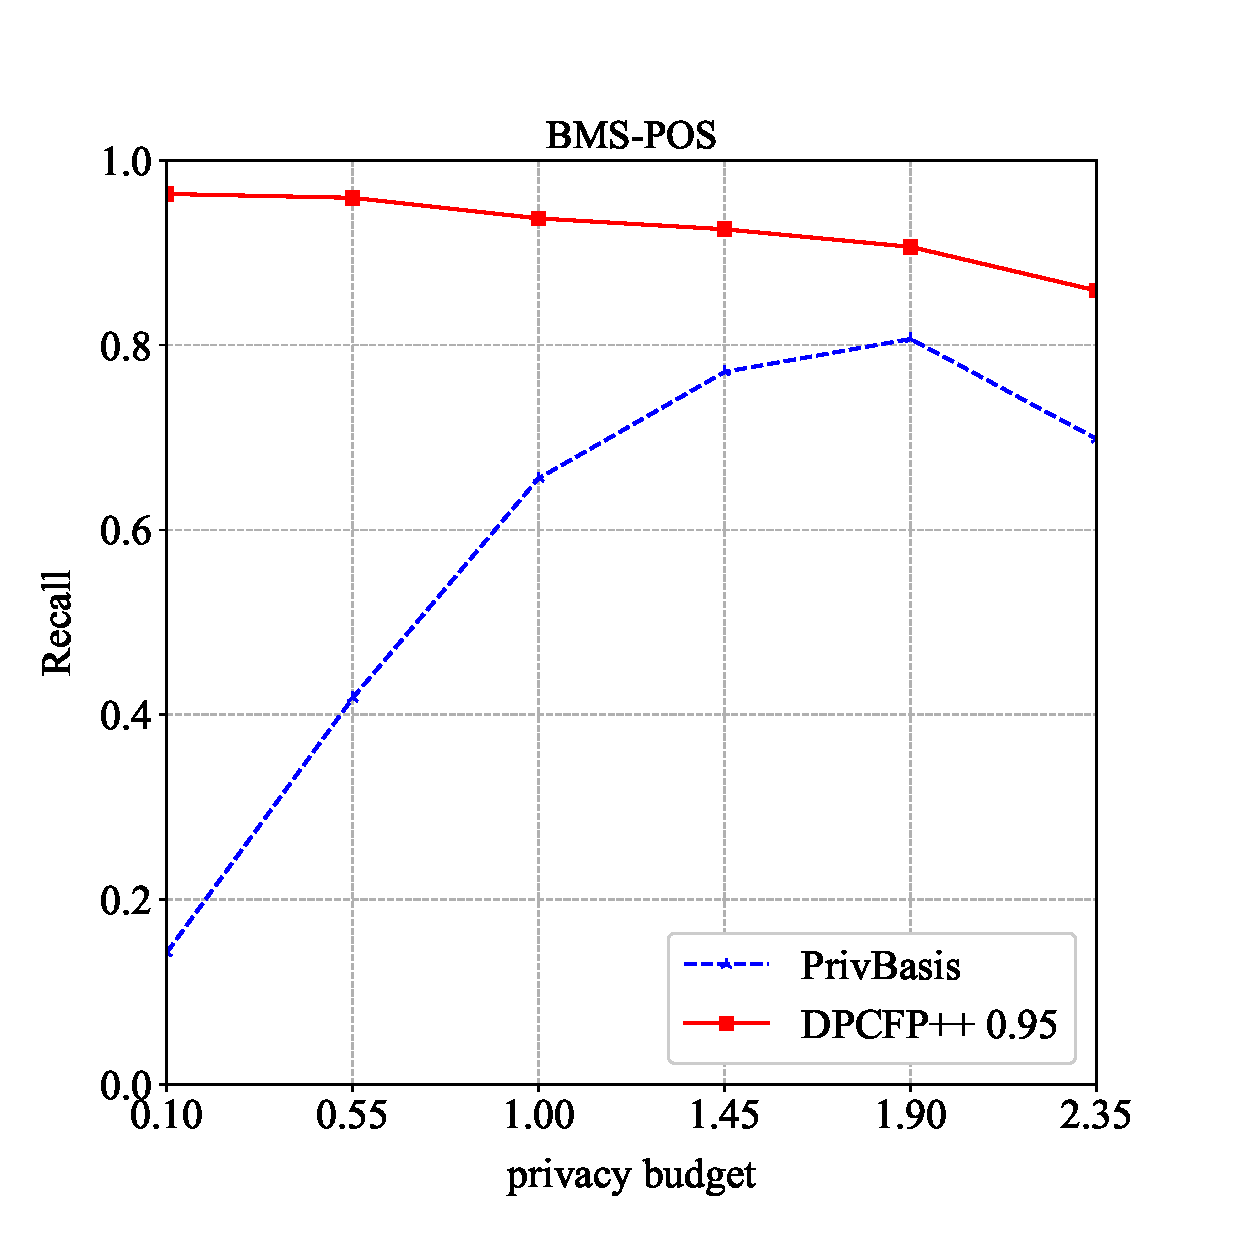
\includegraphics[width=4.5cm]{Recall_BMS-POS.eps}
    }
    \\
    \subfloat[Kosarak]{
        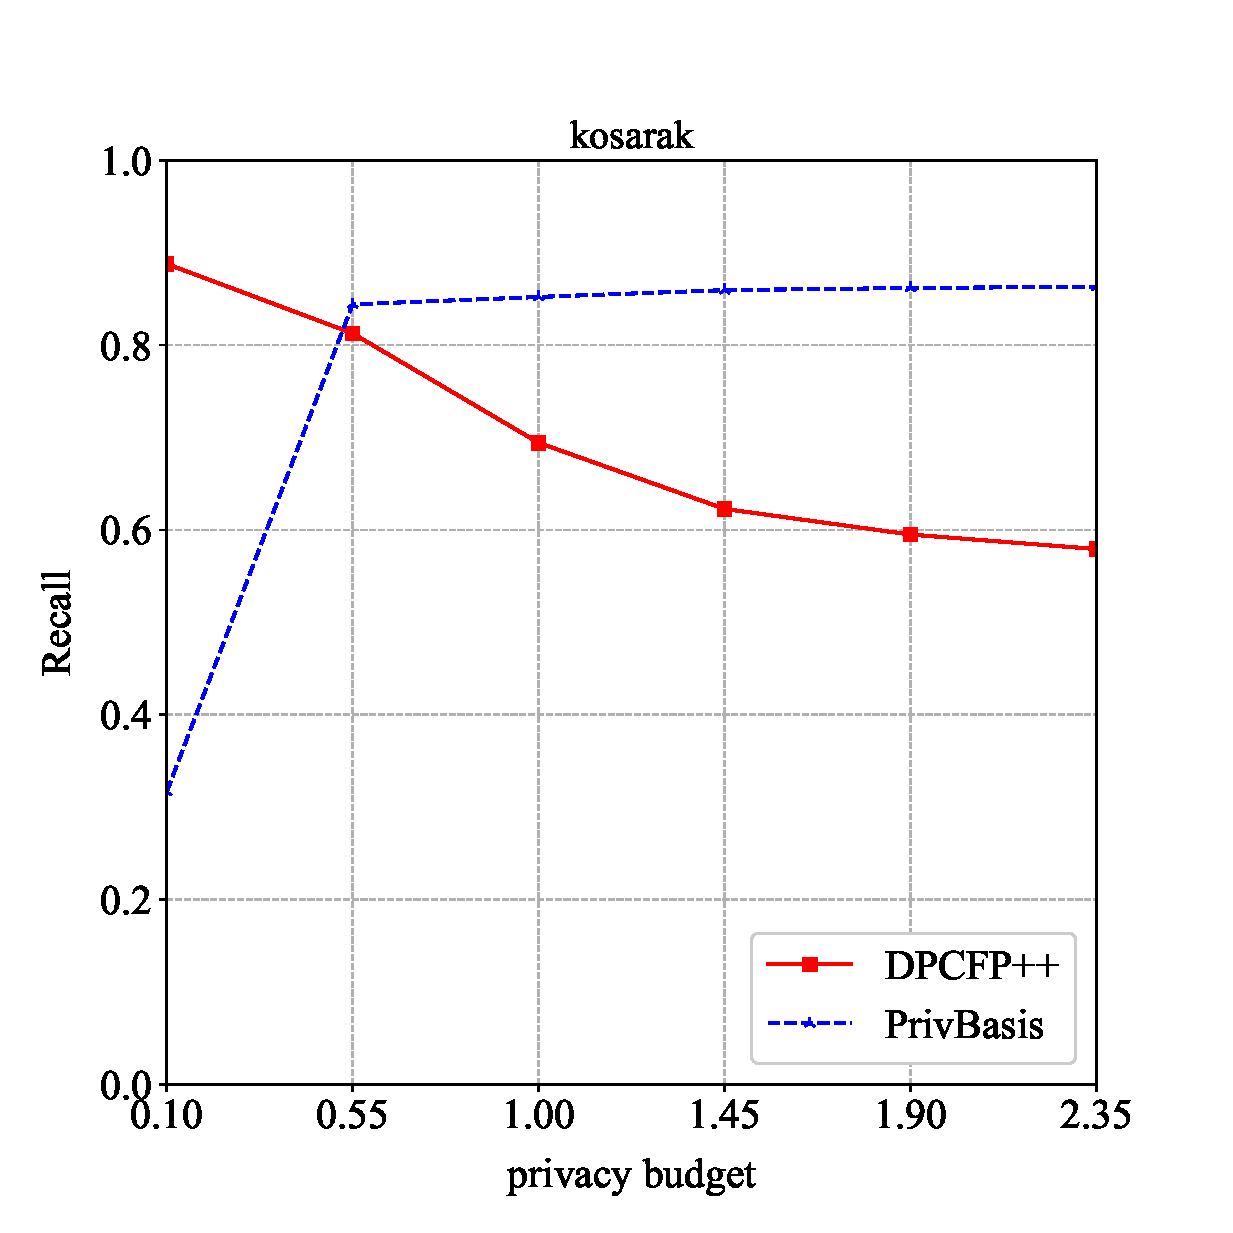
\includegraphics[width=4.5cm]{Recall_kosarak.eps}
    }
    \hfill
    \subfloat[Retail]{
        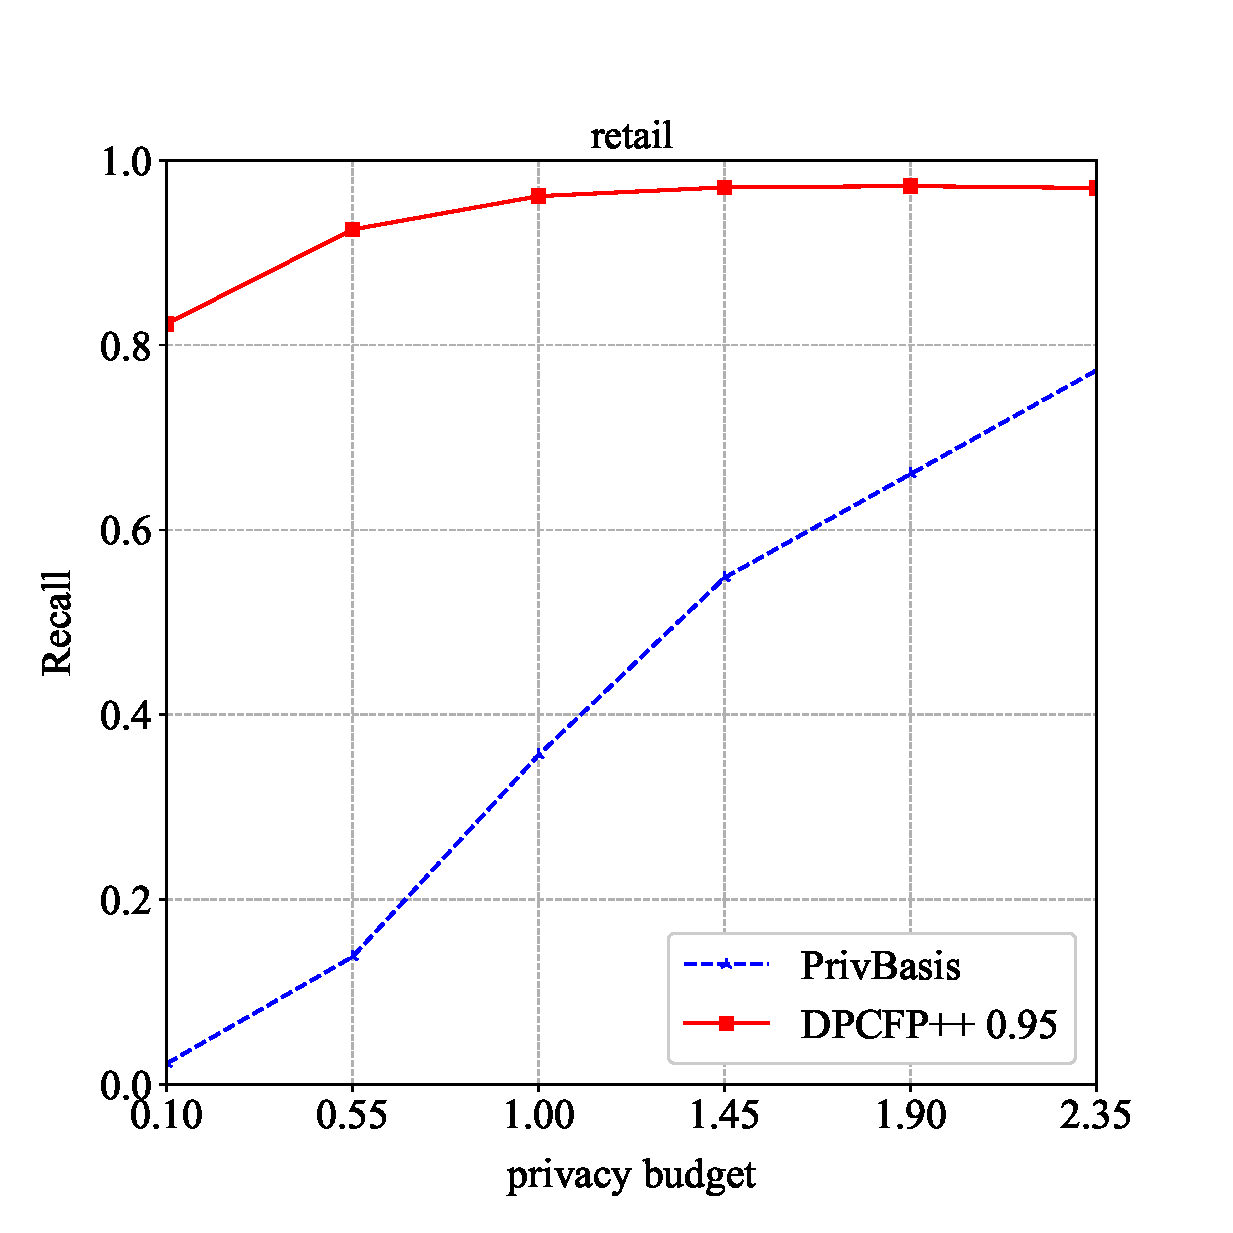
\includegraphics[width=4.5cm]{Recall_retail.eps}
    }
    \hfill
    \subfloat[T10I4D100K]{
        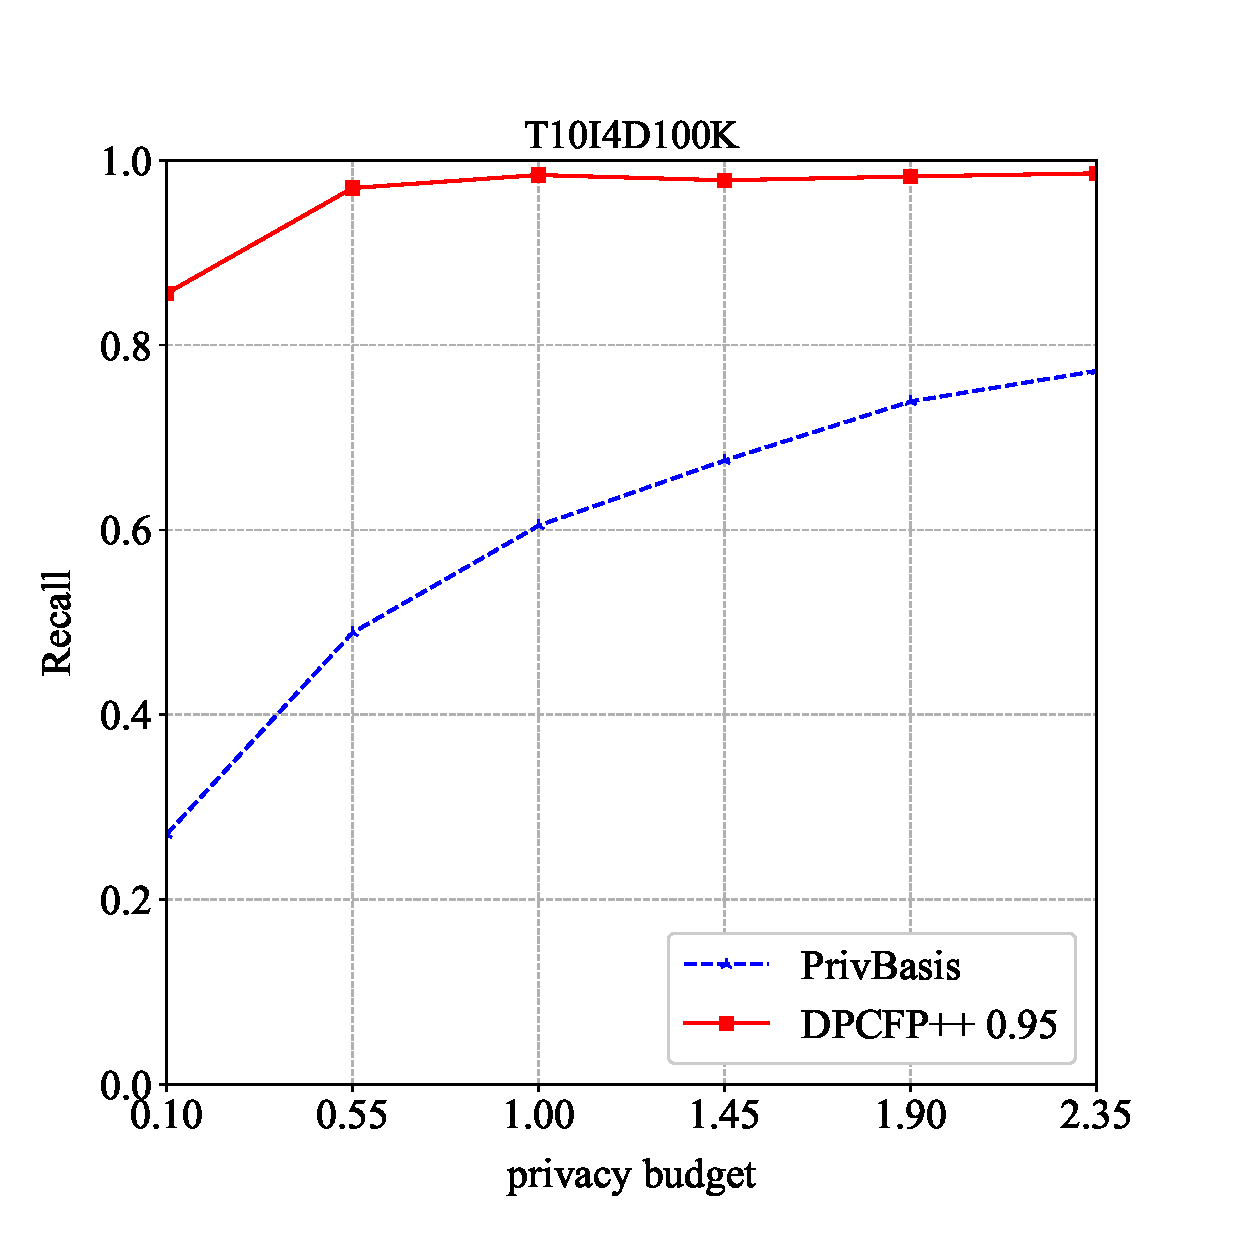
\includegraphics[width=4.5cm]{Recall_T10I4D100K.eps}
    }
\caption{Recall}
\label{Recall}
\end{figure*}

\begin{figure*}[tb]
    \centering
    \subfloat[BMS1]{
        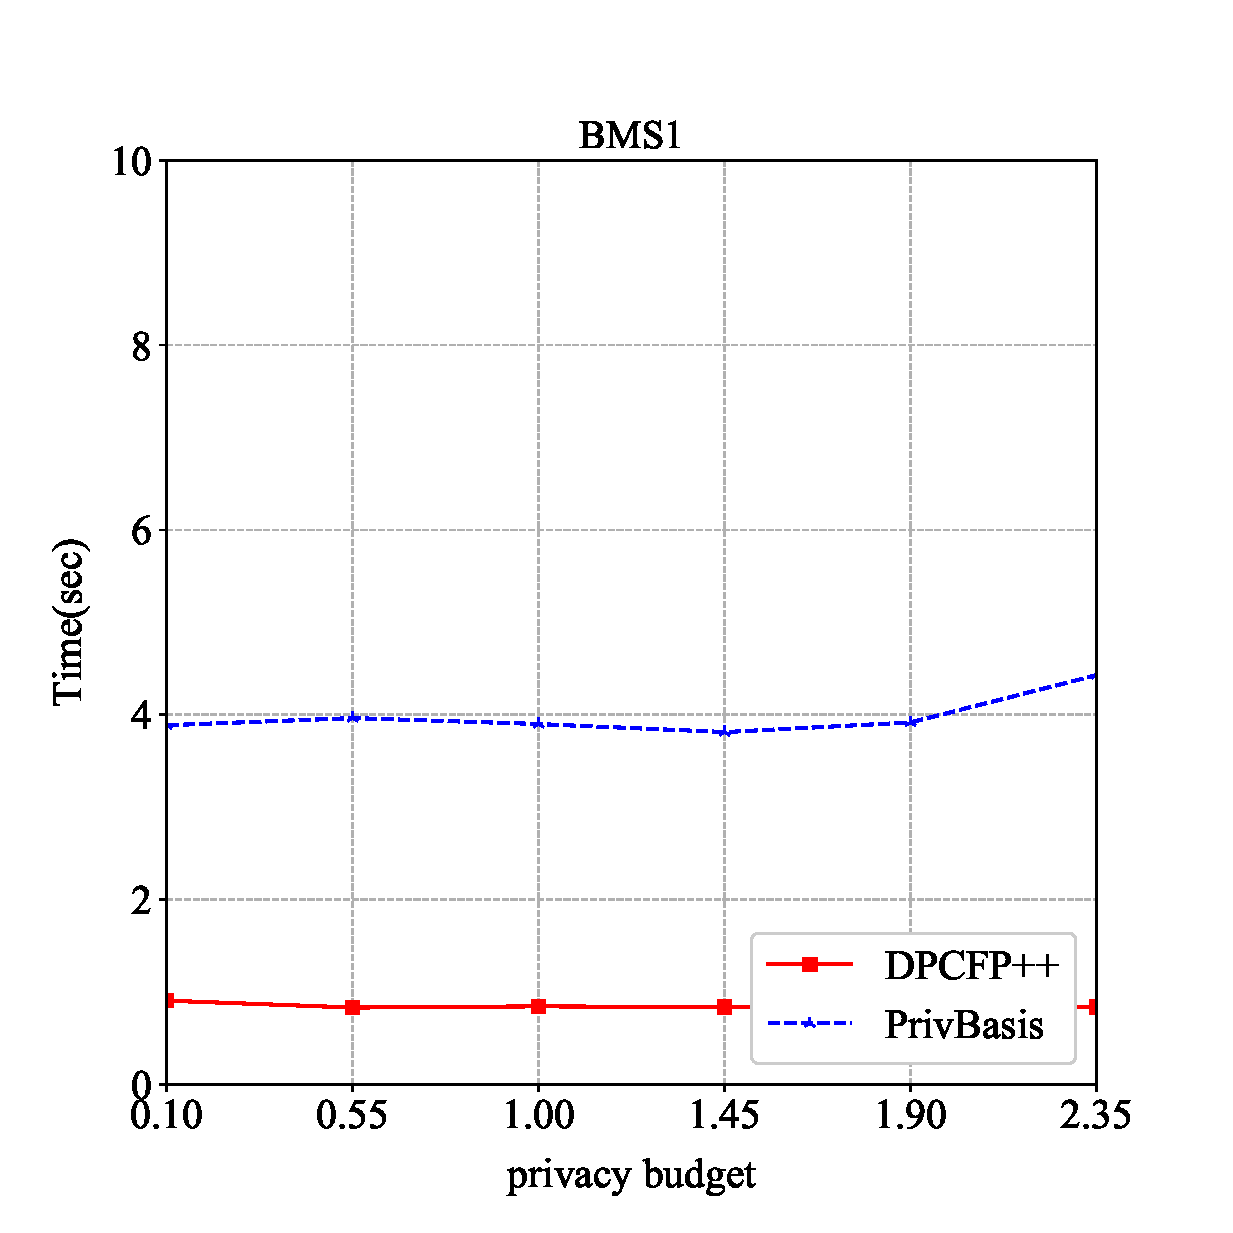
\includegraphics[width=4.5cm]{Runtime_BMS1.eps}
    }
    \hfill
    \subfloat[BMS2]{
        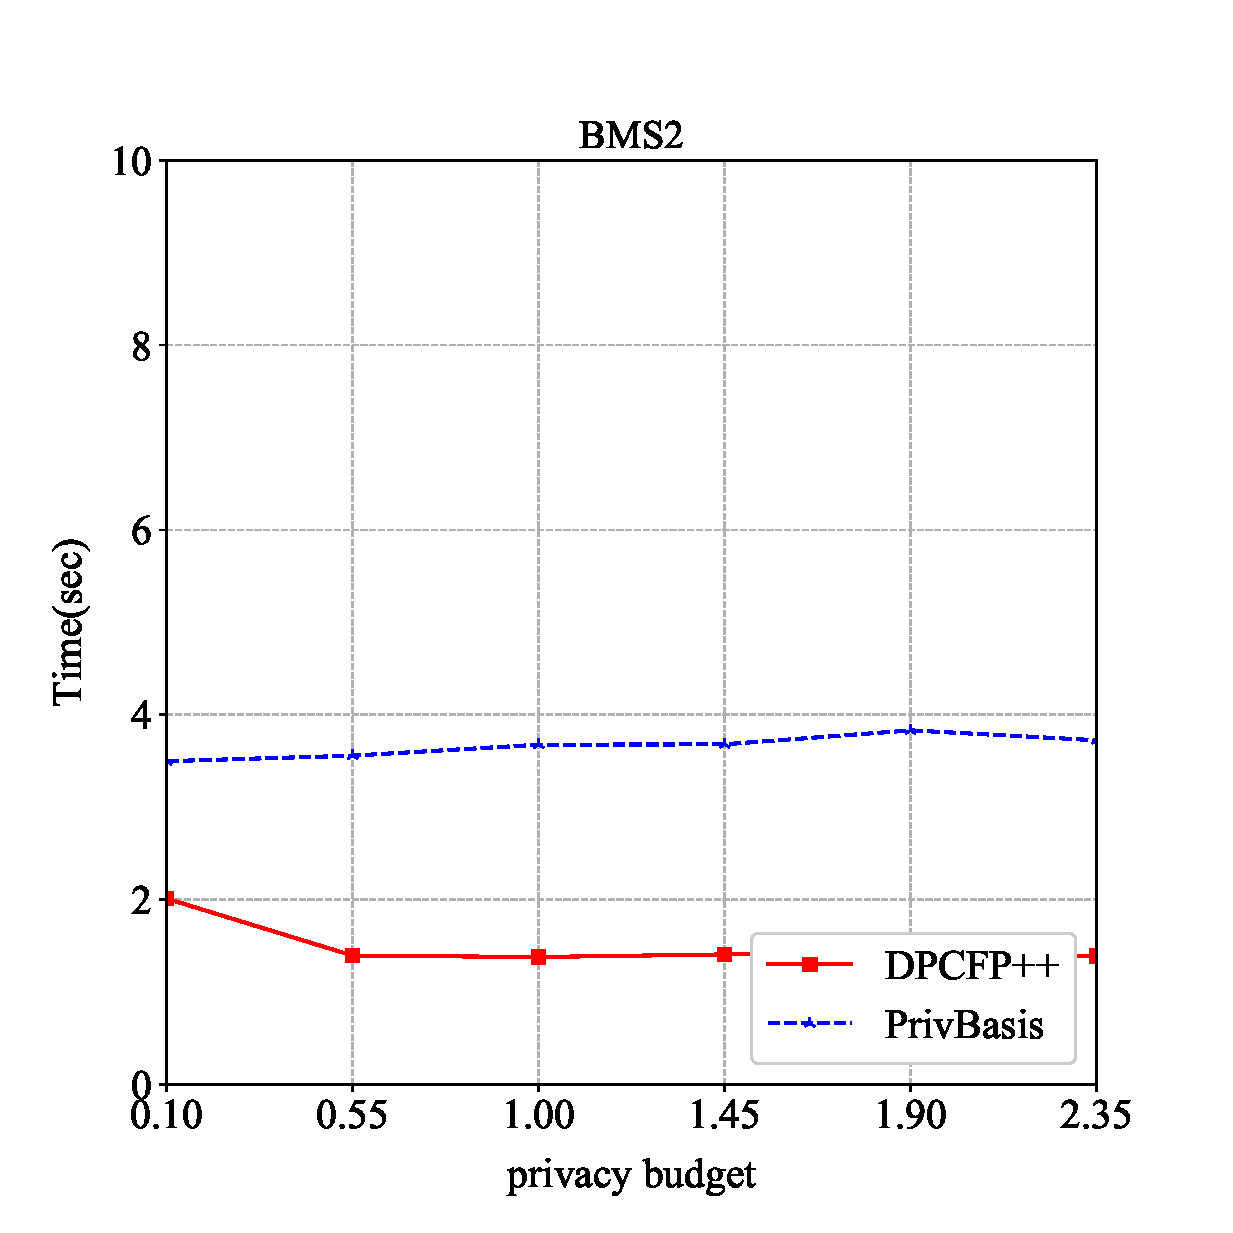
\includegraphics[width=4.5cm]{Runtime_BMS2.eps}
    }
    \hfill
    \subfloat[BMS-POS]{
        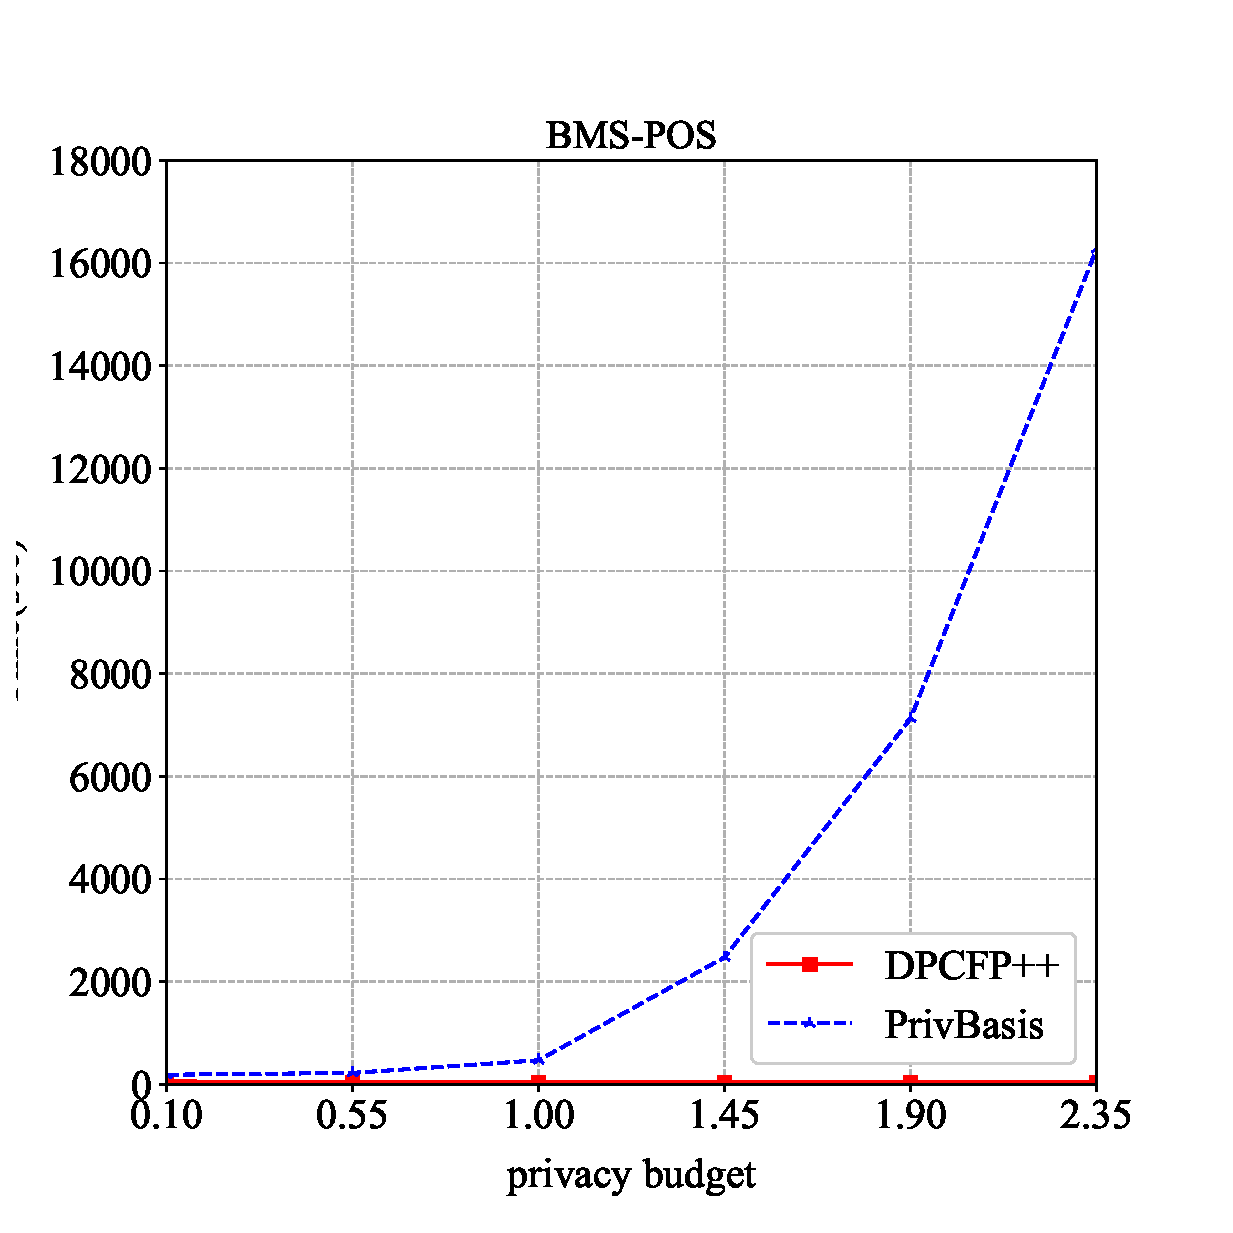
\includegraphics[width=4.5cm]{Runtime_BMS-POS.eps}
    }
    \\
    \subfloat[Kosarak]{
        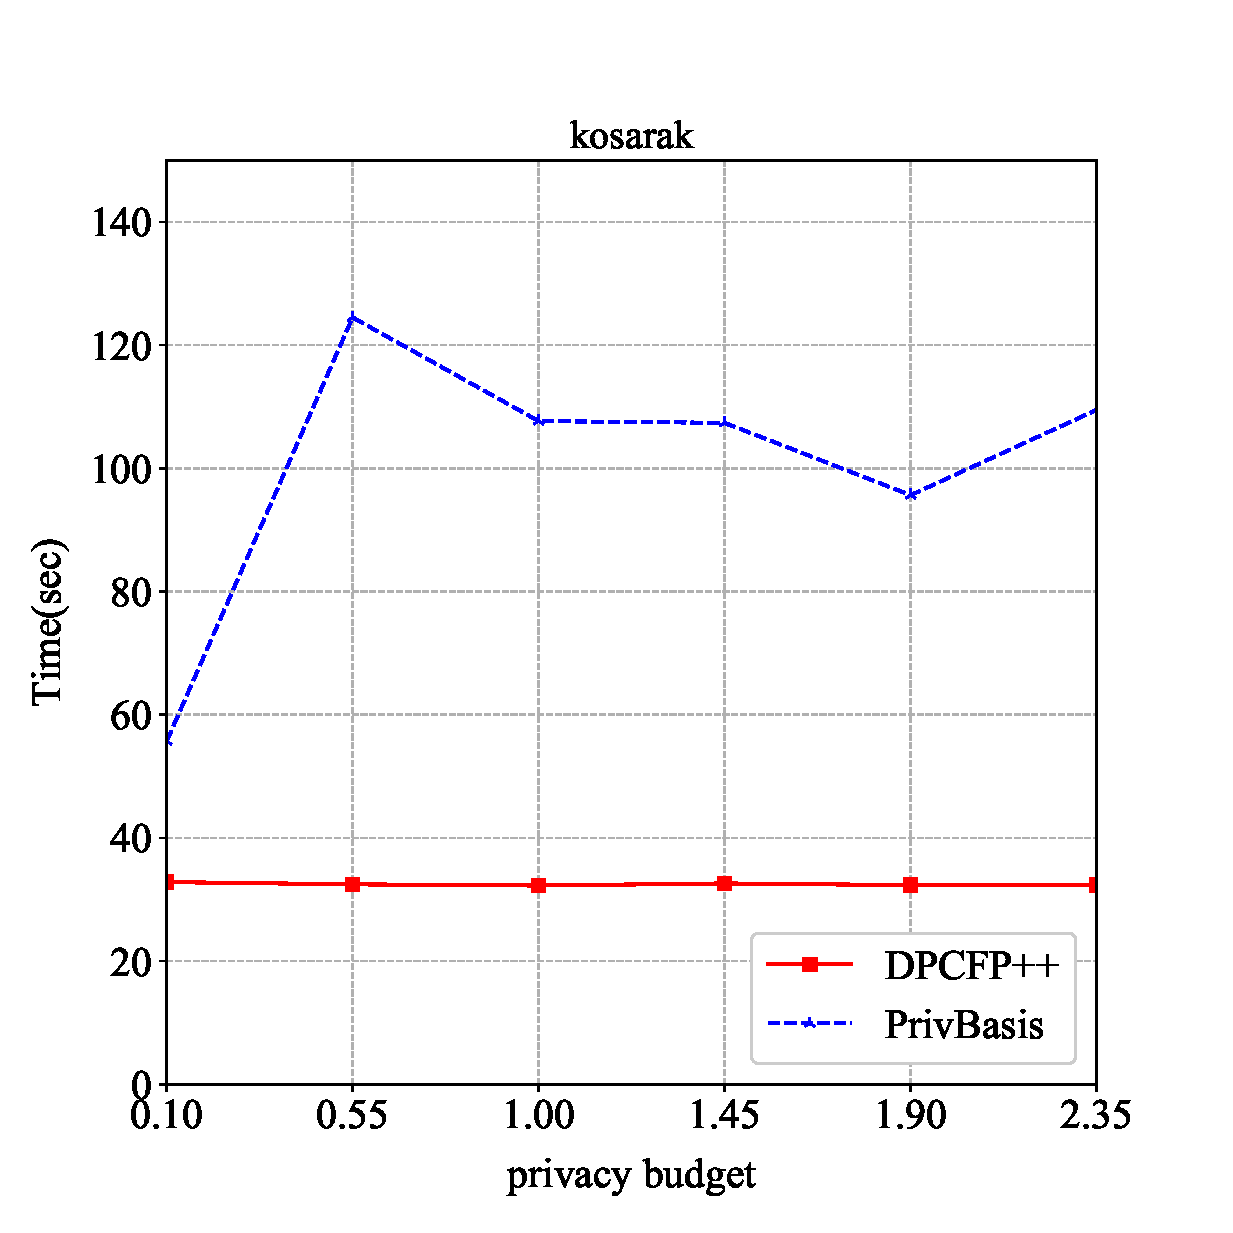
\includegraphics[width=4.5cm]{Runtime_kosarak.eps}
    }
    \hfill
    \subfloat[Retail]{
        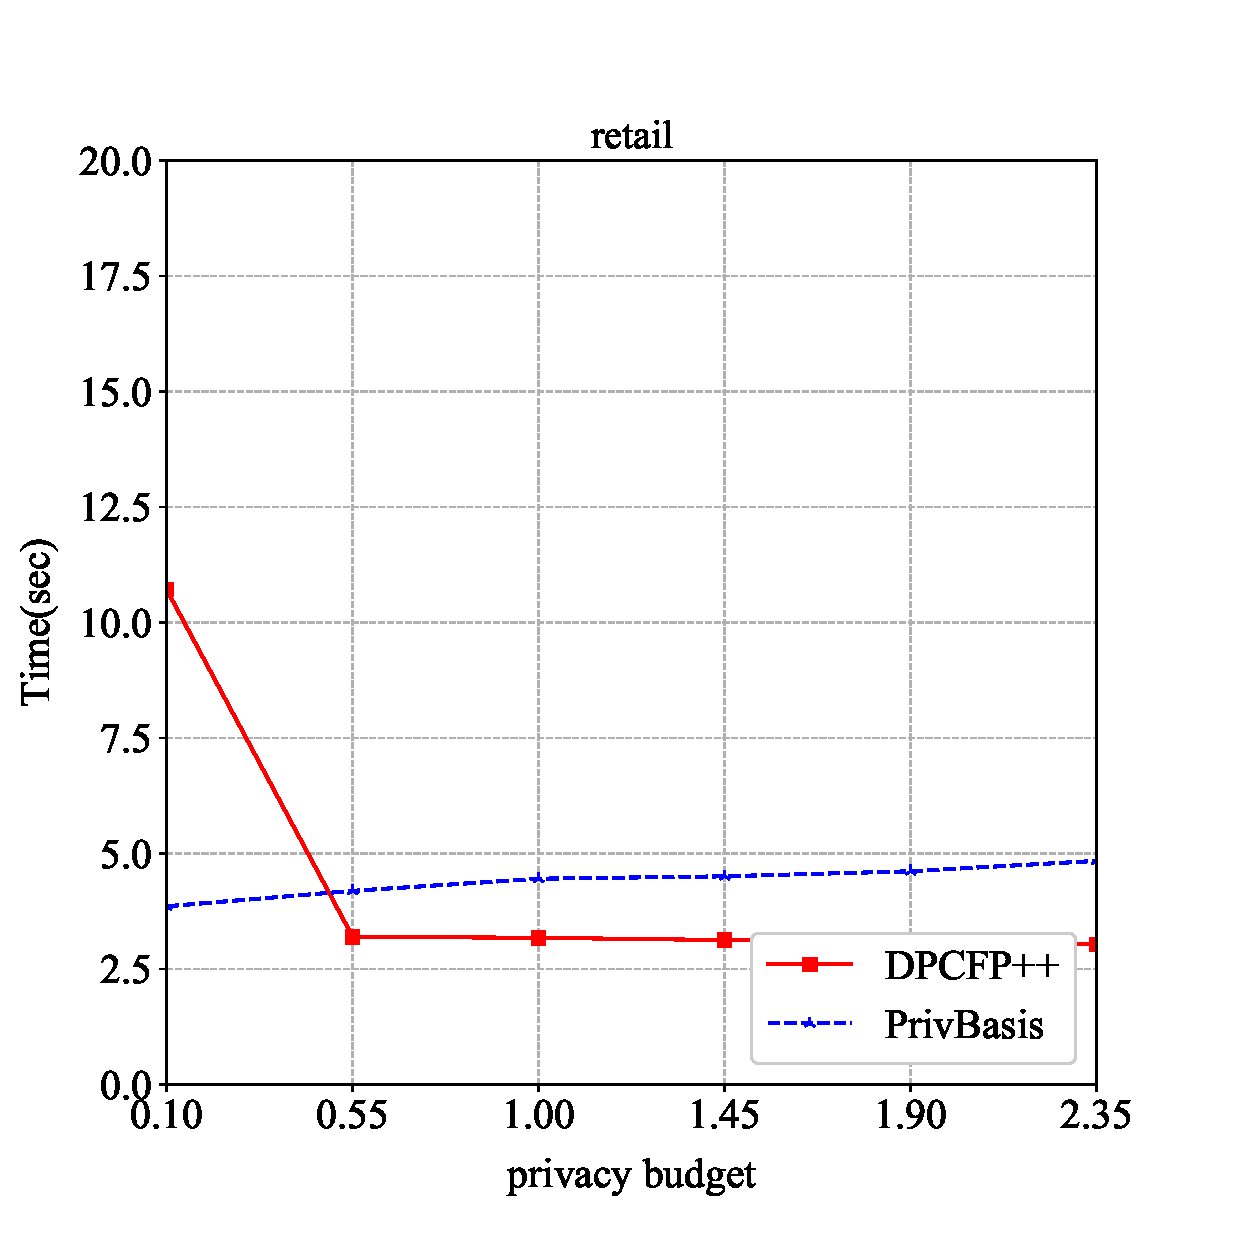
\includegraphics[width=4.5cm]{Runtime_retail.eps}
    }
    \hfill
    \subfloat[T10I4D100K]{
        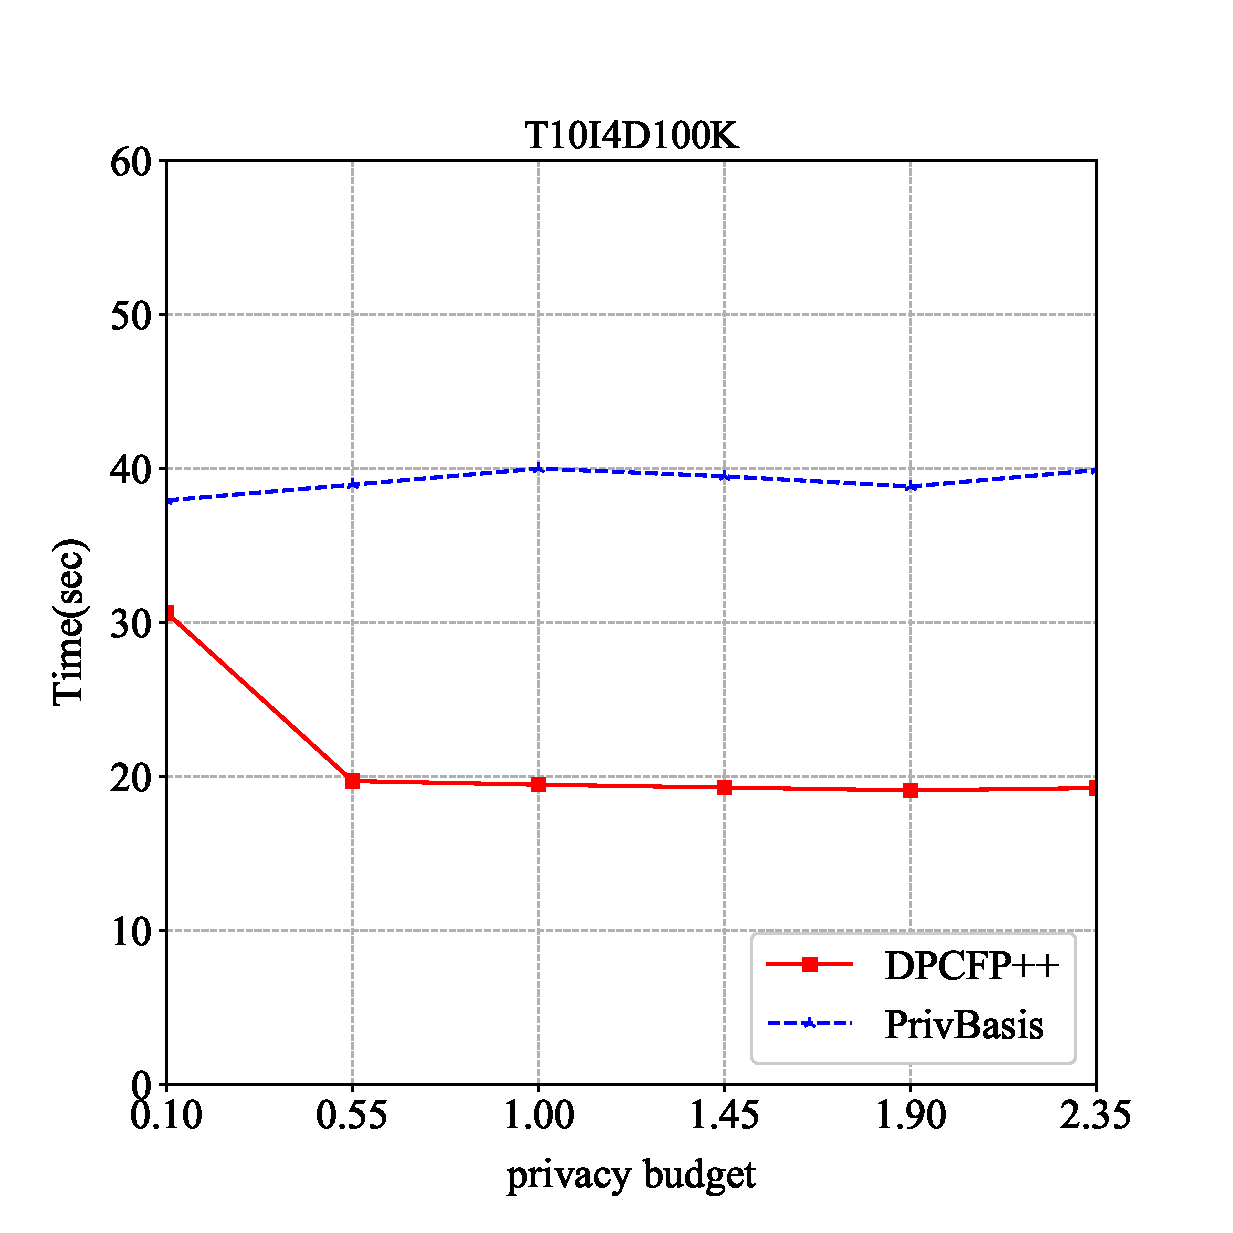
\includegraphics[width=4.5cm]{Runtime_T10I4D100K.eps}
    }
\caption{Runtime}
\label{runtime}
\end{figure*}

% \begin{figure*}[tb]
%     \centering
%     \begin{minipage}[t]{0.3\textwidth}
%     \centering
%     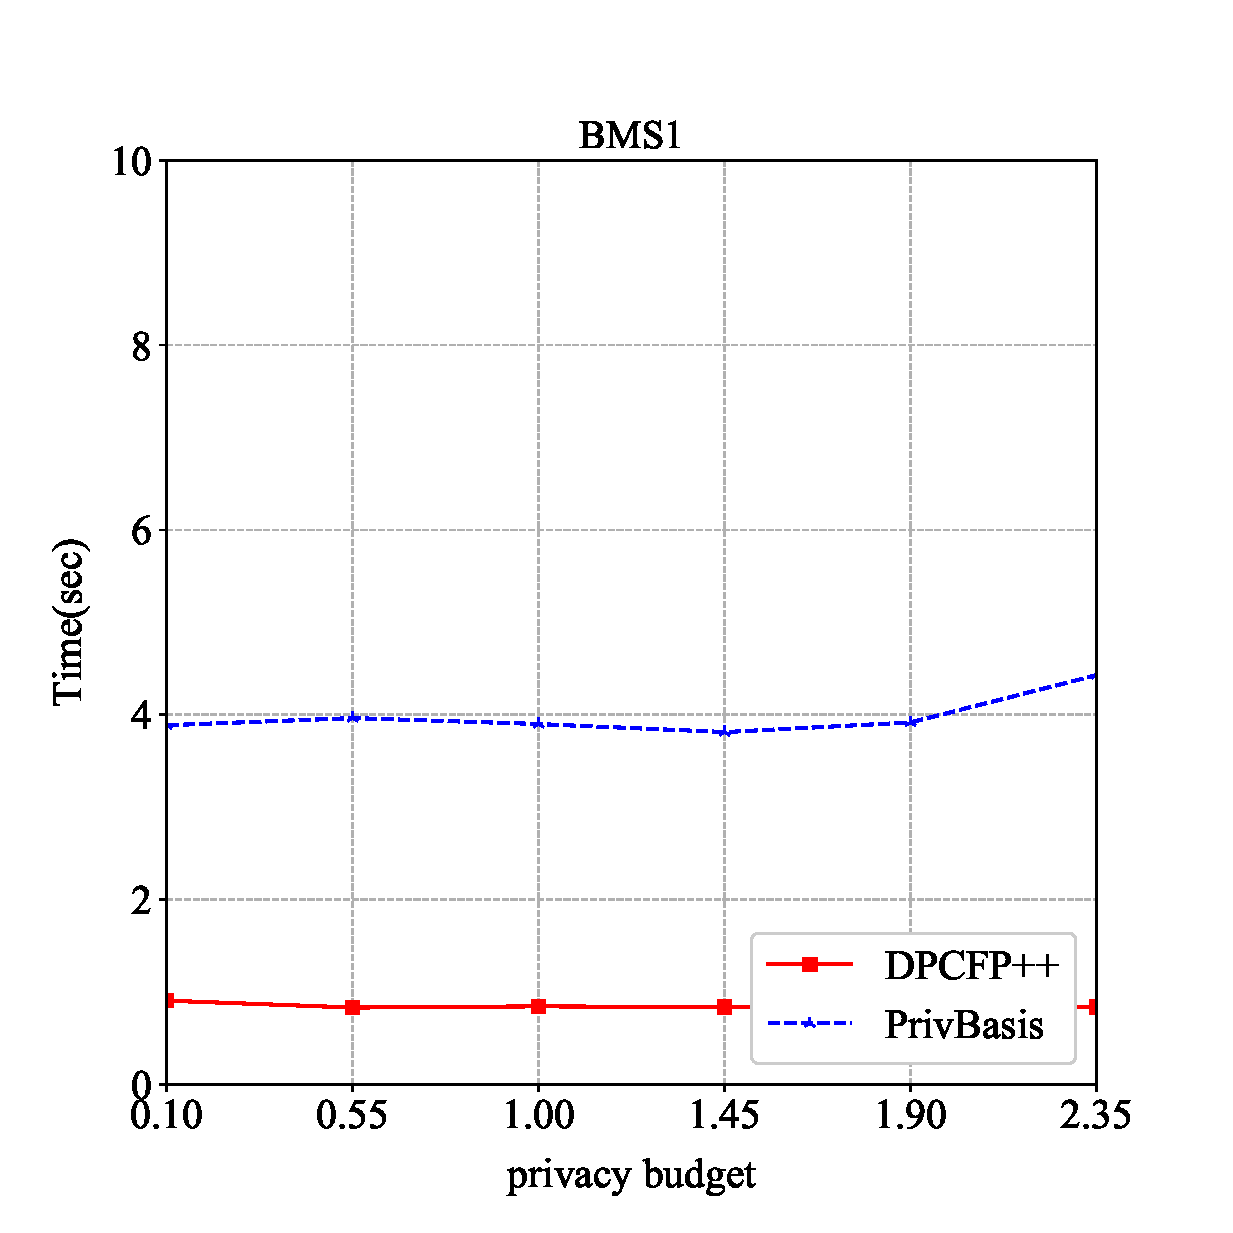
\includegraphics[width=5cm]{Runtime_BMS1.eps}
%     % \subcaption{BMS1}
%     \end{minipage}
%     \hfill
%     \begin{minipage}[t]{0.3\textwidth}
%     \centering
%     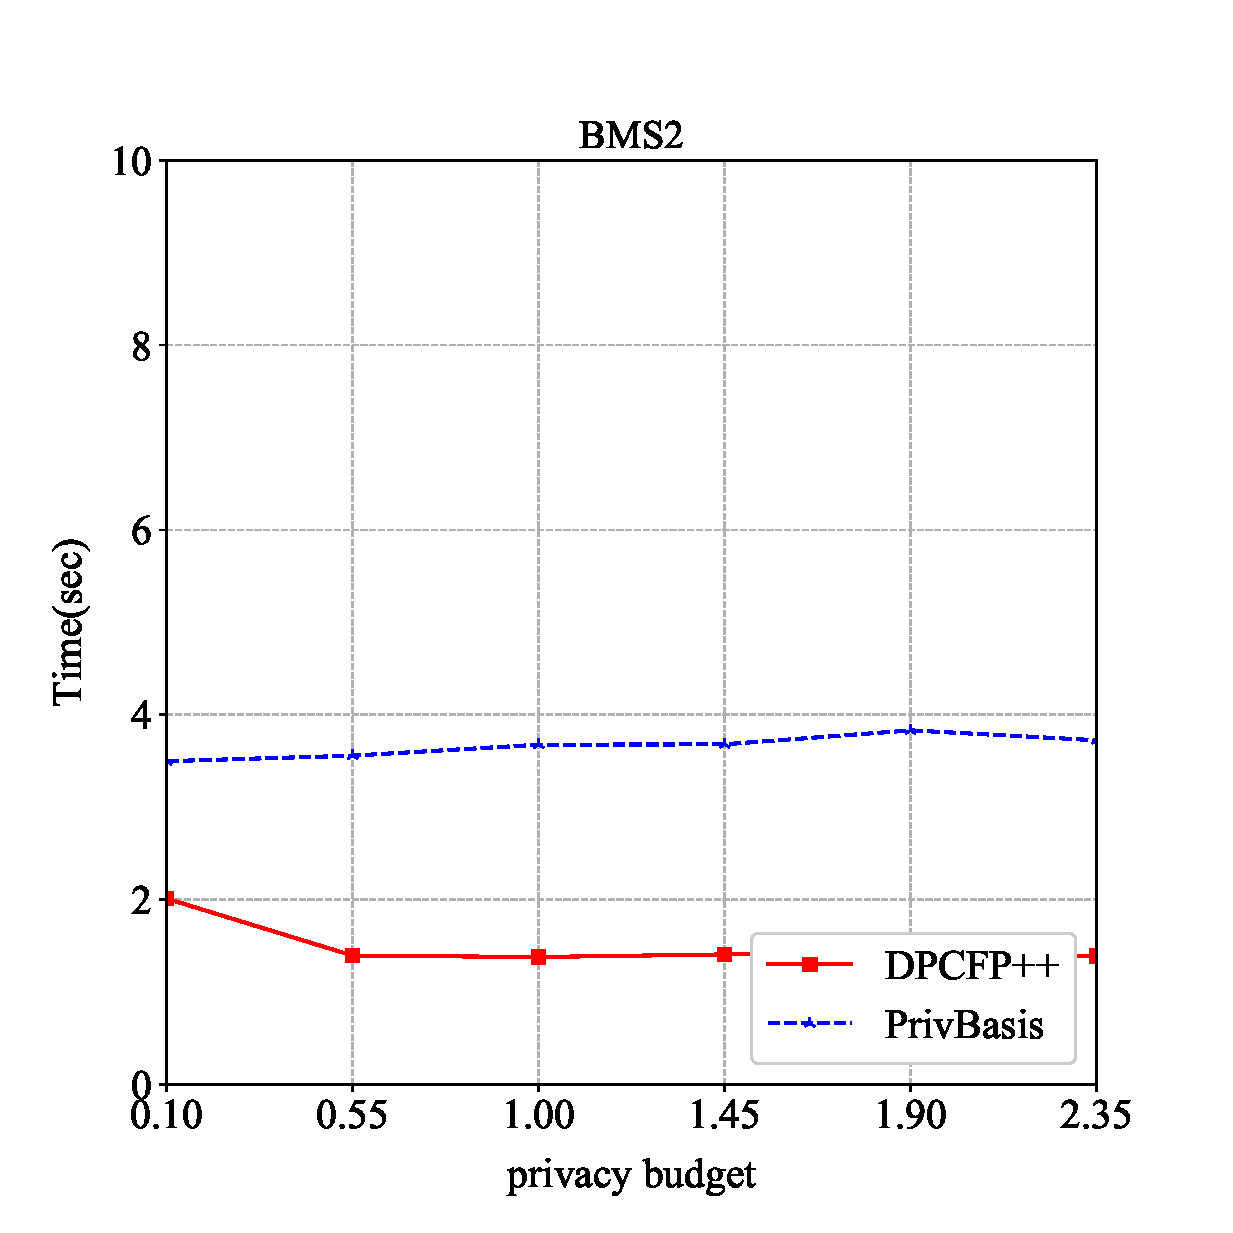
\includegraphics[width=5cm]{Runtime_BMS2.eps}
%     % \subcaption{BMS2}
%     \end{minipage}
%     \hfill
%     \begin{minipage}[t]{0.3\textwidth}
%     \centering
%     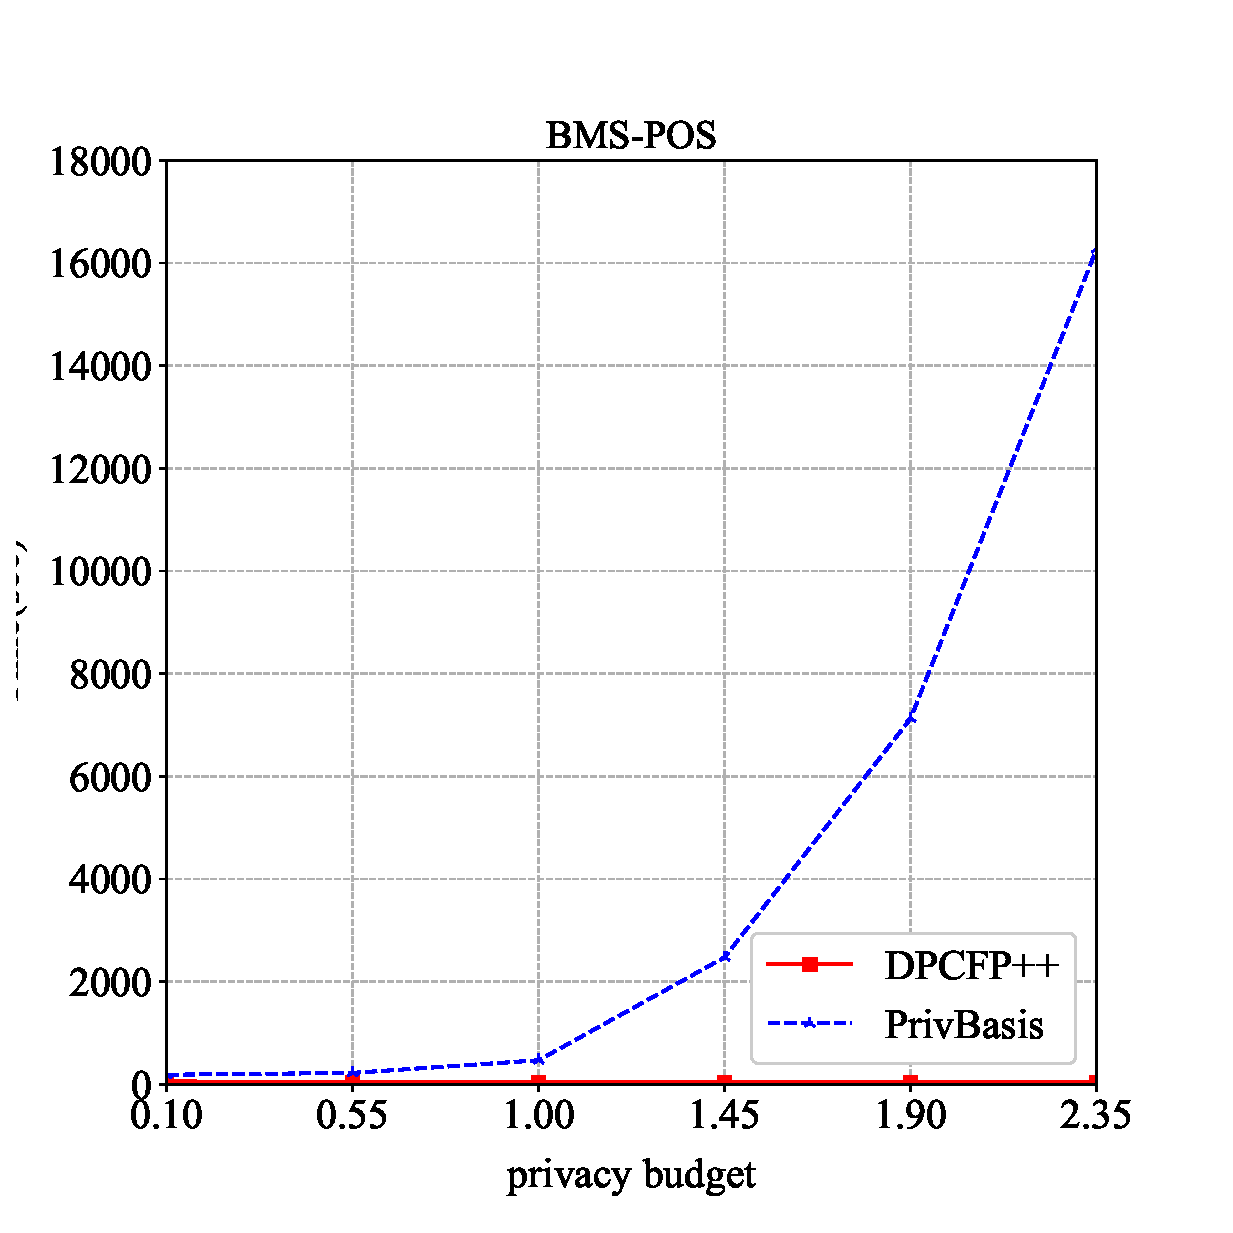
\includegraphics[width=5cm]{Runtime_BMS-POS.eps}
%     % \subcaption{BMS-POS}
%     \end{minipage}
    
%     \begin{minipage}[t]{0.3\textwidth}
%     \centering
%     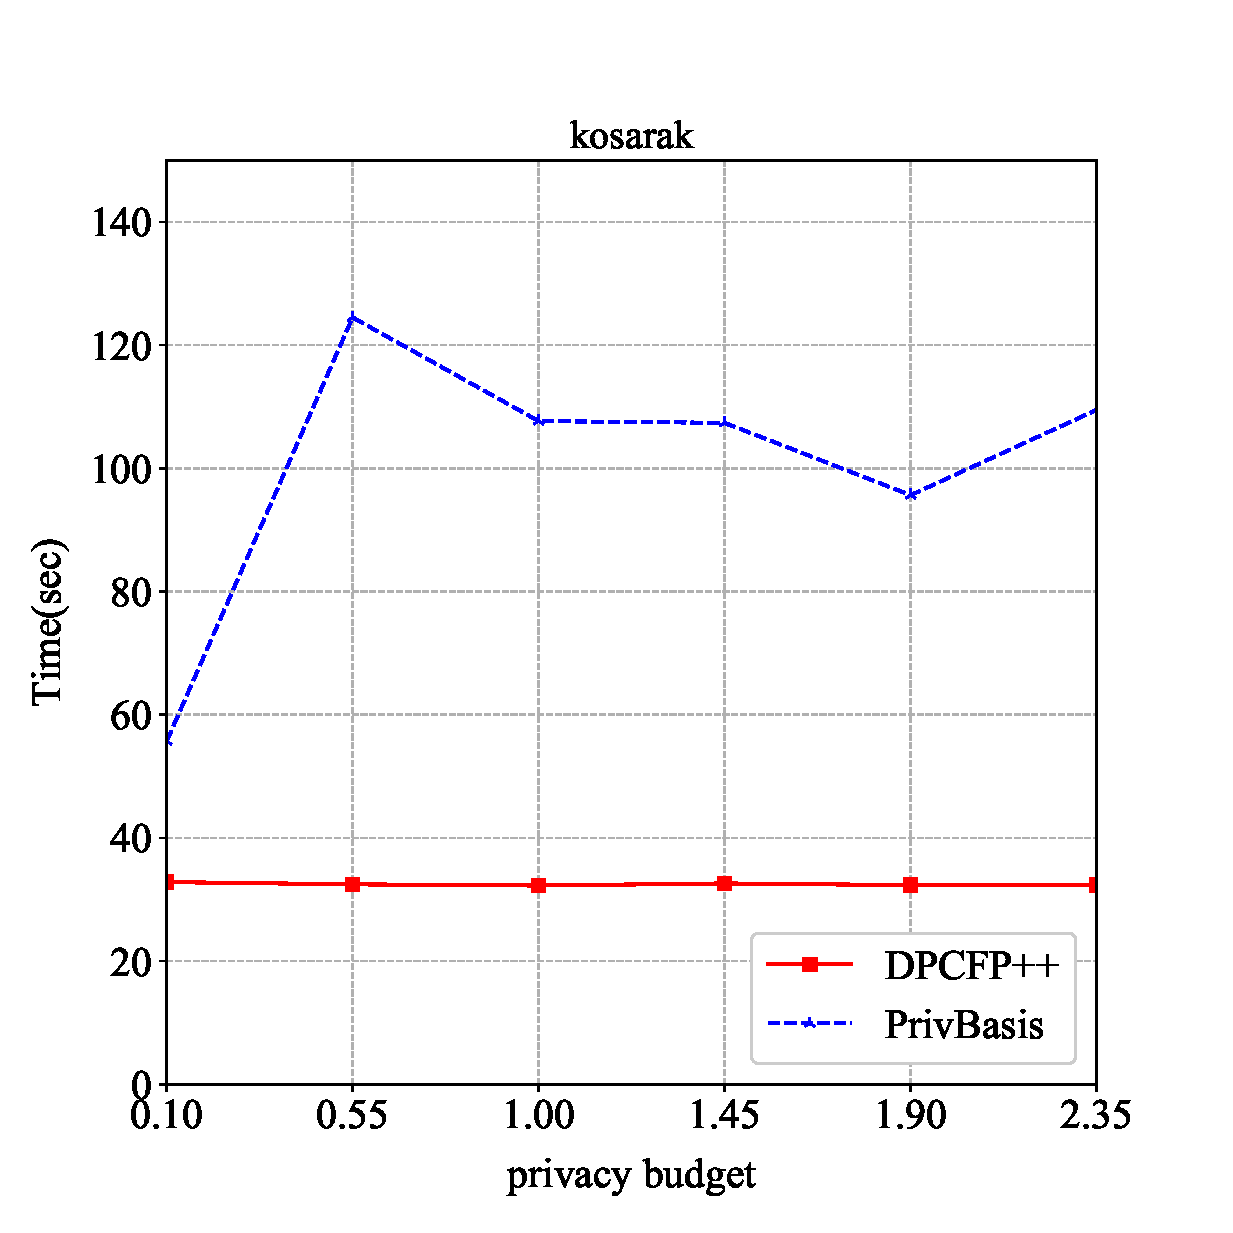
\includegraphics[width=5cm]{Runtime_kosarak.eps}
%     % \subcaption{Kosarak}
%     \end{minipage}
%     \hfill
%     \begin{minipage}[t]{0.3\textwidth}
%     \centering
%     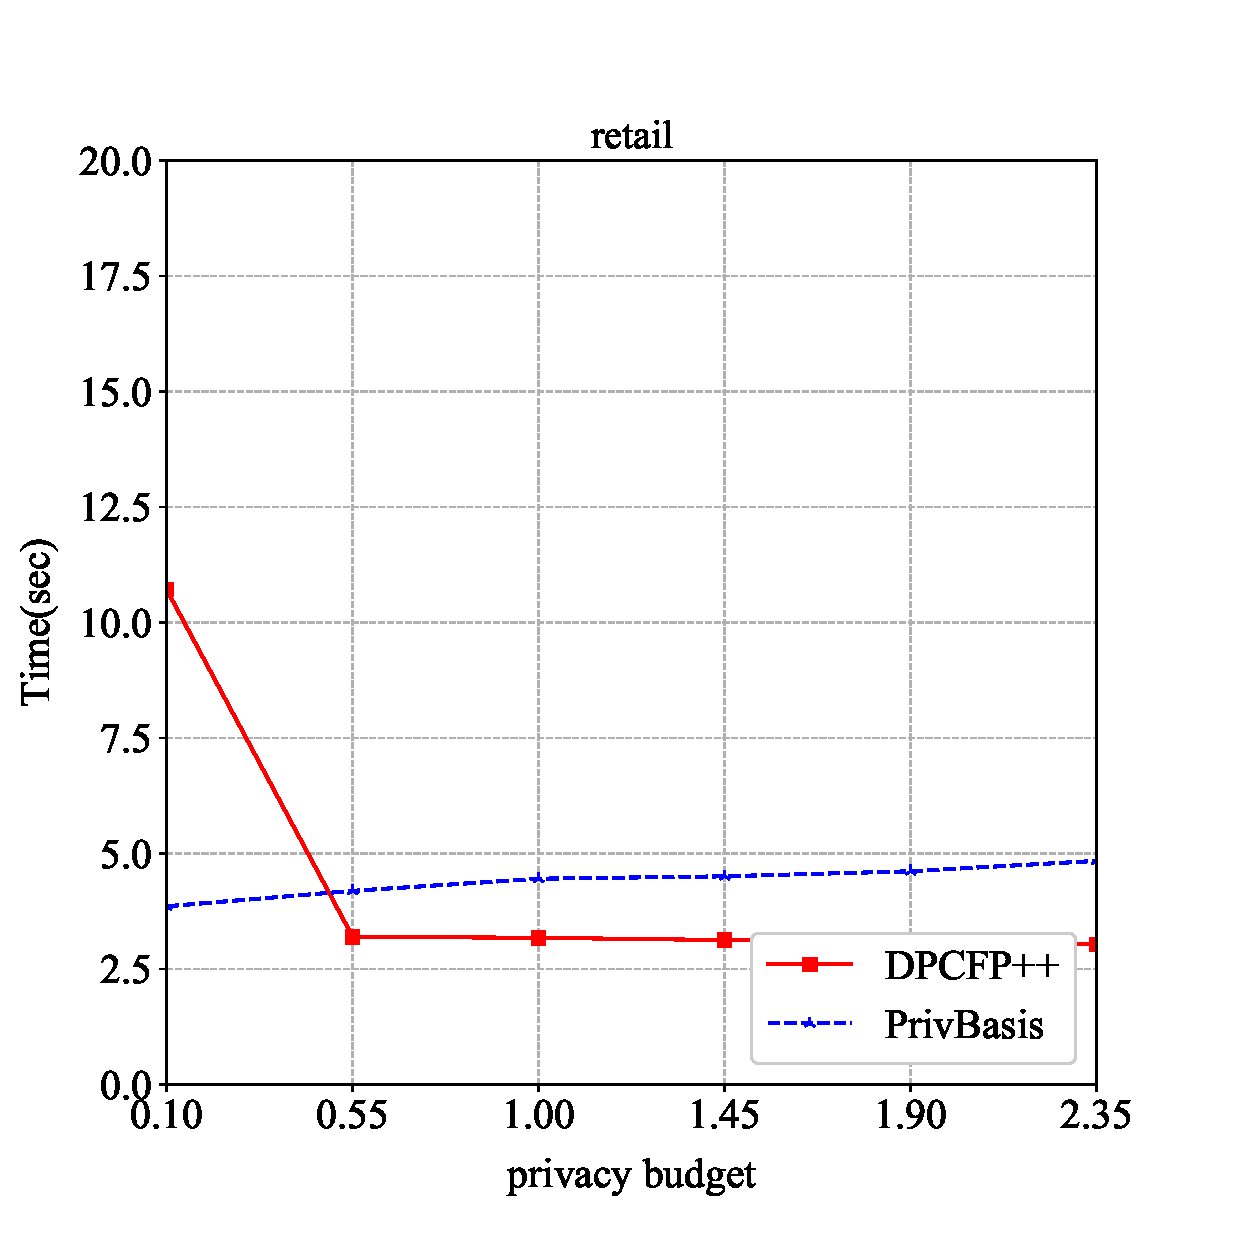
\includegraphics[width=5cm]{Runtime_retail.eps}
%     %\subcaption{Retail}
%     \end{minipage}
%     \hfill
%     \begin{minipage}[t]{0.3\textwidth}
%     \centering
%     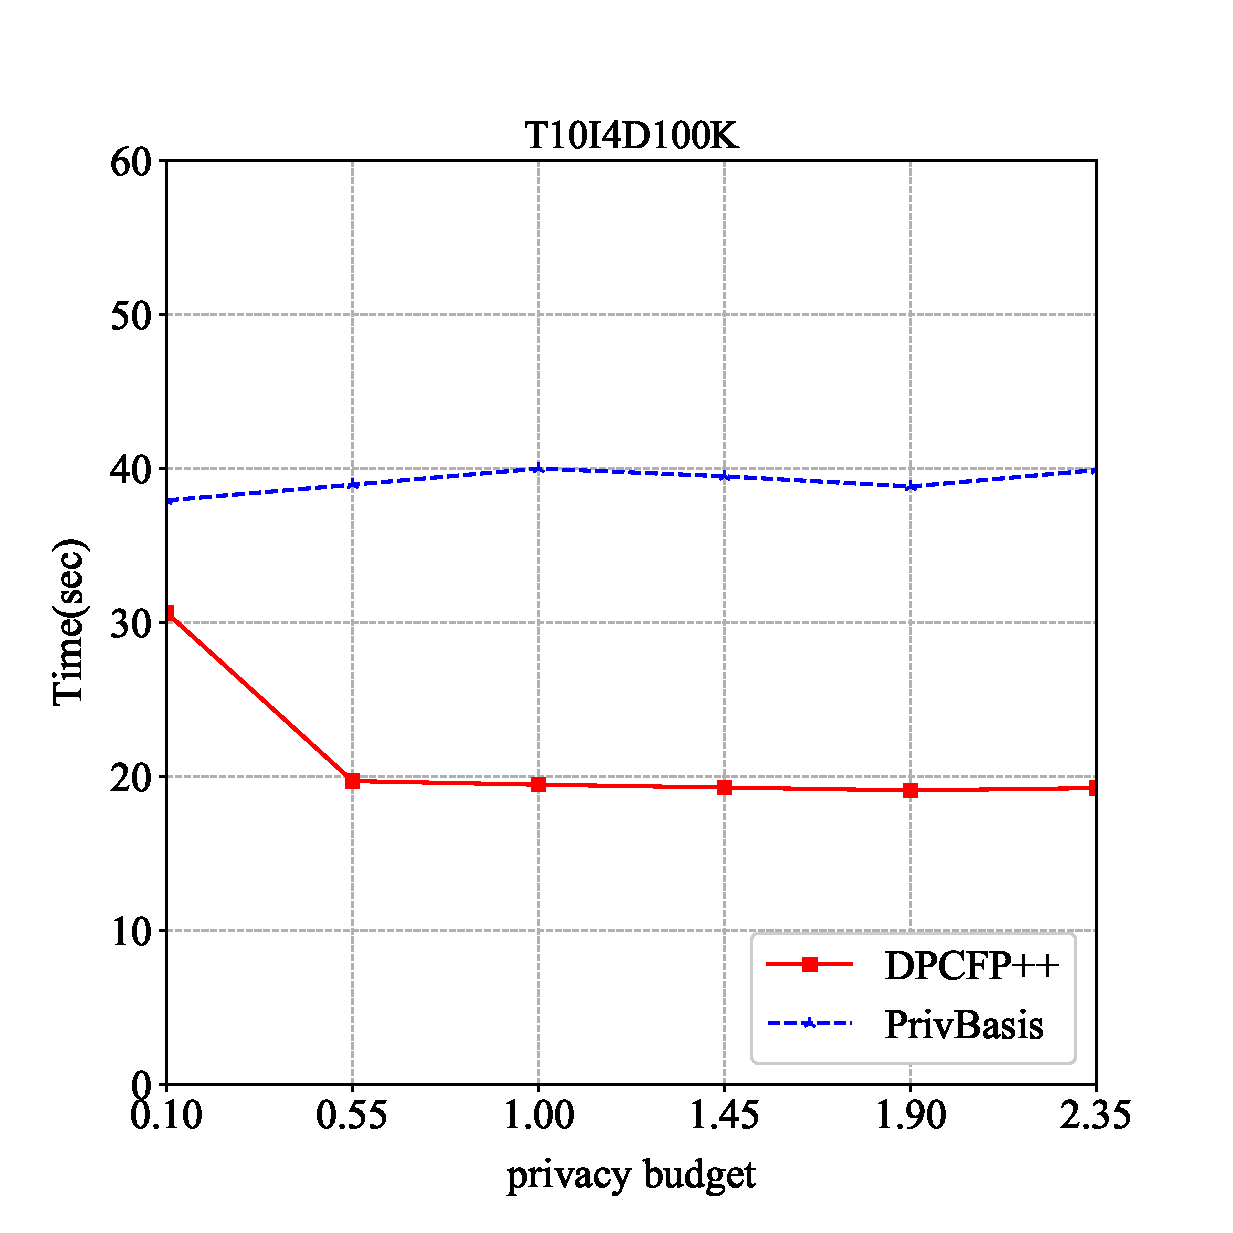
\includegraphics[width=5cm]{Runtime_T10I4D100K.eps}
%     %\subcaption{T10I4D100K}
%     \end{minipage}
% \caption{Runtime}
% \label{runtime}
% \end{figure*}

% \section*{References}

% Please number citations consecutively within brackets \cite{b1}. The 
% sentence punctuation follows the bracket \cite{b2}. Refer simply to the reference 
% number, as in \cite{b3}---do not use ``Ref. \cite{b3}'' or ``reference \cite{b3}'' except at 
% the beginning of a sentence: ``Reference \cite{b3} was the first $\ldots$''

% Number footnotes separately in superscripts. Place the actual footnote at 
% the bottom of the column in which it was cited. Do not put footnotes in the 
% abstract or reference list. Use letters for table footnotes.

% Unless there are six authors or more give all authors' names; do not use 
% ``et al.''. Papers that have not been published, even if they have been 
% submitted for publication, should be cited as ``unpublished'' \cite{b4}. Papers 
% that have been accepted for publication should be cited as ``in press'' \cite{b5}. 
% Capitalize only the first word in a paper title, except for proper nouns and 
% element symbols.

\section{Conclusion}\label{sec6}
In this paper, we propose DPCFP-growth++, a novel differentially private algorithm for frequent itemset mining with multiple minimum supports. 

The algorithm is composed of three stages. 
The total privacy budget follows sequential composition theorem of differential privacy.
In order to find frequent 1-itemsets and assign MIS, we first differential privately limit the length of transactions by random truncation to reduce the sensitivity. 
Secondly, we apply Laplace noise to the accumulated support counts of truncated transactions.
After that, we store the information of the database into a differentially private MIS-tree.
Finally, by using regular DPCFP-growth++ algorithm, we can uncover the frequent itemsets.

From the experiments on real-world and synthetic datasets, 
we find our algorithm DPCFP-growth++ significantly outperforms current algorithm and achieves both high utility and high efficiency. 

As for future work, there are some directions that we can utilize. 
First of all, extend our work to high-utility itemset mining. 
High-utility mining is an advanced setting of frequent itemset mining. 
It takes the purchase quantities into account. 
User can set unit profit for each item, and the total utility can be computed by the sum of the products of the quantities and unit profits.
Literatures such as \cite{b22} adapted FP-growth-like algorithms which is similar to our work.

Secondly, reduce the information loss. 
Transaction splitting method in \cite{b20} seems a better idea than simply truncate transactions. 
More specifically, it splits a long transaction into multiple pieces of small transcations and add them into the database while the random truncating method just neglects the items that are above length constraint.
However, it needs more time to preprocess the dataset and may drastically slow down the total mining process.



\begin{thebibliography}{21}%論文標題只有第一個字大寫
    \bibitem{b1} R. Agrawal, T. Imielinski, and A. Swami. ``Mining association rules between sets of items in large databases,'' in Proceedings of the 1993 ACM SIGMOD international conference on Management of data (SIGMOD '93), pp. 207-216, 1993.
    \bibitem{b2} B. Liu, W. Hsu, and Y. Ma. ``Mining association rules with multiple minimum supports,'' in Proceedings of the 5th ACM SIGKDD international conference on Knowledge discovery and data Mining(KDD '99), 1999.
    \bibitem{b3} Y. Hu, and Y. Chen. ``Mining association rules with multiple minimum supports: a new mining algorithm and a support tuning mechanism,'' in Decision Support System, vol. 42, no. 1, pp. 1-24, 2006.
    \bibitem{b4} R. Uday Kiran, and P. Krishna Reddy. ``Novel techniques to reduce search space in multiple minimum supports-based frequent pattern mining algorithms,'' in Proceedings of the 14th International Conference on Extending Database Technology (EDBT/ICDT '11), pp. 11-20, 2011.
    \bibitem{b5} W. Gan, J. C.-W. Lin, P. Fournier-Viger, H. Chao, and J. Zhan. ``Mining of frequent patterns with multiple minimum supports,'' in Engineering Applications of Artificial Intelligence, vol. 60, pp. 83-96, 2017.
    \bibitem{b6} C. Zeng, J. F. Naughton, and J. -Y. Cai. ``On differentially private frequent itemset mining,'' in Proceedings of the VLDB Endowment, vol. 6, no. 1, pp. 25-36, 2012.
    \bibitem{b7} N. Li, W. H. Qardaji, D. Su, and J. Cao. ``PrivBasis: Frequent itemset mining with differential privacy,'' in Proceedings of the VLDB Endowment, vol. 5, no. 11, pp. 1340-1351, 2012.
    \bibitem{b8} J. Lee and C. W. Clifton. ``Top-k frequent itemsets via differentially private fp-trees,'' in Proceedings of the 20th ACM SIGKDD international conference on Knowledge discovery and data Mining(KDD '14), 2014.
    \bibitem{b9} C. Dwork. ``Differential privacy,'' in 33rd International Colloquium on Automata, Languages and Programming (ICALP), pp.1-12, 2006.
    \bibitem{b10}Y. Chen and A. Machanavajjhala. ``On the privacy properties of variants on the sparse vector technique,'' in CoRR, 2015.
    \bibitem{b11}J. Zhang, X. Xiao, and X. Xie. ``PrivTree: A differentially private algorithm for hierarchical decompositions,'' in Proceedings of the 2016 International Conference on Management of Data (SIGMOD '16), pp. 155-170, 2016.
    \bibitem{b12}Frequent Itemset Mining Implementations Repository. http://fimi.uantwerpen.be/data/, 2004
    \bibitem{b13}A. Narayanan and V. Shmatikov. ``Robust de-anonymization of large sparse datasets,'' in IEEE Symposium on Security and Privacy (S \&P), pp. 111-125, 2008.
    \bibitem{b14}P. Fournier-Viger, J.C.-W. Lin, B. Vo, T.T. Chi, J.Zhang, and H.B. Le. ``A survey of itemset mining,'' in WIREs Data Mining and Knowledge Discovery,vol. 7, no. 4, 2017.
    \bibitem{b15}T. Zhu, G. Li, W.Zhou, P. S. Yu. ``Differentially private data publishing and analysis: a survey,'' in IEEE Transactions on Knowledge and Data Engineering (TKDE), vol. 29, no. 8, pp. 1619-1638, 2017.
    \bibitem{b16}R. Agrawal, R. Srikant. ``Fast algorithms for mining association rules,''in Proceedings of the 20th International Conference on Very Large Data Bases (VLDB '94), pp. 487-499, 1994.
    \bibitem{b17}J. Han, J. Pei, and Y. Yin. ``Mining frequent patterns without candidate generation,'' in Proceedings of the 2000 ACM SIGMOD international conference on Management of data (SIGMOD '00), pp. 1-12, 2000.
    \bibitem{b18}Y.-H. Hu and Y.-L. Chen. ``Mining association rules with multiple minimum supports: a new mining algorithm and a support tuning mechanism,'' in Decision Support System, vol. 42, no. 1, pp. 1–24, 2006.
    \bibitem{b19}R. Bhaskar, S. Laxman, A. Smith, and A. Thakurta. ``Discovering frequent patterns in sensitive data,'' in Proceedings of the 16th ACM SIGKDD international conference on Knowledge discovery and data mining (KDD '10), pp. 503–512, . 2010.
    \bibitem{b20}S. Su, S. Xu, X. Cheng, Z. Li and F. Yang. ``Differentially private frequent itemset mining via transaction splitting,'' in IEEE Transactions on Knowledge and Data Engineering (TKDE), vol. 27, no. 7, pp. 1875-1891, 2015.
    \bibitem{b21}N. Wang, X. Xiao, Y. Yang, Z. Zhang, Y. Gu and G. Yu. ``PrivSuper: a superset-first approach to frequent itemset mining under differential privacy,''in 2017 IEEE 33rd International Conference on Data Engineering (ICDE), pp. 809-820, 2017.
    \bibitem{b22}V. S. Tseng, C. Wu, B. Shie, and P. S. Yu. ``UP-Growth: An efficient algorithm for high utility itemset mining,'' in Proceedings of the 16th ACM SIGKDD international conference on Knowledge discovery and data Mining(KDD '10), pp. 253–262, 2010.
\end{thebibliography}


\end{document}
